\documentclass[10pt,notes,compress,aspectratio=169]{beamer}
\usepackage[brazil]{babel}  
\usepackage[utf8]{inputenc}
\usepackage[T1]{fontenc}

\usefonttheme[onlymath]{serif}
\usepackage{beamerthemesplit}
\usetheme{Antibes}

\beamersetuncovermixins{\opaqueness<1->{25}}{\opaqueness<2->{15}}
\setbeamertemplate{itemize items}[triangle]
\setbeamertemplate{enumerate item}{\insertenumlabel)}
\setbeamertemplate{enumerate subitem}{\insertenumlabel-\insertsubenumlabel)}
\setbeamertemplate{caption}[numbered]
\setbeamertemplate{mini frames}{}
\setbeamertemplate{navigation symbols}{}
\setbeamerfont{block title}{size=\scriptsize}
\setbeamerfont{frametitle}{size=\small}
\beamertemplatenavigationsymbolsempty

%%%%%%%%%%%%%%%%%%%%%
% defining frametitle
\setbeamertemplate{frametitle}{%
    \nointerlineskip%
    \begin{beamercolorbox}[wd=\paperwidth,ht=2.5ex,dp=1.0ex]{frametitle}
        \hspace*{2.5ex}\insertframetitle%
    \end{beamercolorbox}%
}
%%%%%%%%%%%%%%%%%%%%%

\newcommand{\hrefcolor}[2]{\textcolor{BlueGreen}{\href{#1}{#2}}}

% Rotating Objects and Captions
\usepackage{hvfloat}

\usepackage{natbib}
\usepackage[brazilian]{cleveref}
\crefname{lstlisting}{lista}{listas}
\Crefname{lstlisting}{Lista}{Listas}

% equation stuff
\usepackage{nicefrac}
\usepackage{cancel}

% table diagonal box
\usepackage{diagbox}
\usepackage{makecell}

% tables
\usepackage{booktabs}

% BEGIN - listings - code in LaTeX
\usepackage{listings}
\renewcommand\lstlistingname{Lista}
\lstset{
  language=octave,
  breaklines=true,
  postbreak=\mbox{$\hookrightarrow$\space},
  basicstyle=\linespread{1}\small\ttfamily,
  %numbers=left,
  numbers=none,
  %frame=lines,
  xleftmargin=0.5cm,
  frame=none,
  framexleftmargin=0.5em,
  framexrightmargin=0.5em,
  %backgroundcolor=\color{light-gray},
  showstringspaces=false,
  upquote=true,
  commentstyle=\color{gray},
  %morecomment=[f][\color{gray}][28]{\#},
  morecomment=[l]{\#\#},
  literate=%
           {á}{{\'a}}1
           {í}{{\'i}}1
           {é}{{\'e}}1
           {ú}{{\'u}}1
           {ó}{{\'o}}1
           {à}{{\`a}}1
           {ã}{{\~a}}1
           {õ}{{\~o}}1
           {â}{{\^a}}1
           {ê}{{\^e}}1
           {ô}{{\^o}}1
           {ç}{{\c{c}}}1
           {Á}{{\'A}}1
           {Í}{{\'I}}1
           {É}{{\'E}}1
           {Ú}{{\'U}}1
           {Ó}{{\'O}}1
           {À}{{\`A}}1
           {Ã}{{\~A}}1
           {Õ}{{\~O}}1
           {Â}{{\^A}}1
           {Ê}{{\^E}}1
           {Ô}{{\^O}}1
           {Ç}{{\c{C}}}1
}
% END - listings

%\usepackage{amsthm}
%\newtheorem{theorem}{Theorem}
%\newtheorem{corollary}{Corollary}
%\newtheorem{lemma}{Lemma}
\newtheorem{proposition}{Proposition}
\newtheorem{axiom}{Axiom}
%\newtheorem{example}{Example}
%\newtheorem{definition}{Definition}
\newtheorem{remark}{Remark}

\usepackage{etoolbox}
\patchcmd{\theorem}{Theorem}{Teorema}{}{}
\patchcmd{\corollary}{Corollary}{Corolário}{}{}
\patchcmd{\lemma}{Lemma}{Lema}{}{}
\patchcmd{\proposition}{Proposition}{Proposição}{}{}
\patchcmd{\axiom}{Axiom}{Axioma}{}{}
\patchcmd{\example}{Example}{Exemplo}{}{}
\patchcmd{\definition}{Definition}{Definição}{}{}
\patchcmd{\remark}{Remark}{Observação}{}{}

%\patchcmd{\theorem}{Theorem}{Teorema}{}{}
%\patchcmd{\corollary}{Corollary}{Corolário}{}{}
%\patchcmd{\lemma}{Lemma}{Lema}{}{}
%\patchcmd{\proposition}{Proposition}{Proposição}{}{}
%\patchcmd{\axiom}{Axiom}{Axioma}{}{}
%\patchcmd{\example}{Example}{Exemplo}{}{}
%\patchcmd{\definition}{Definition}{Definição}{}{}
%\patchcmd{\remark}{Remark}{Observação}{}{}

%\newtheorem{exercise}[theorem]{Exercício}


\newcommand*{\theorembreak}{\usebeamertemplate{theorem end}\framebreak\usebeamertemplate{theorem begin}}
\newcommand*{\proofbreak}{\hfill ...\usebeamertemplate{proof end}\framebreak\usebeamertemplate{proof begin}{\scriptsize\color{gray}continuação...}\\}
\newcommand*{\examplebreak}{\hfill ...\usebeamertemplate{theorem end}\framebreak\usebeamertemplate{theorem begin}{\scriptsize\color{gray}continuação...}\\}
\newcommand*{\exercisebreak}{\hfill ...\usebeamertemplate{theorem end}\framebreak\usebeamertemplate{theorem begin}{\scriptsize\color{gray}continuação...}\\}
\newcommand*{\lemmabreak}{\hfill ...\usebeamertemplate{theorem end}\framebreak\usebeamertemplate{theorem begin}{\scriptsize\color{gray}continuação...}\\}
\newcommand*{\blockbreak}{\hfill ...\usebeamertemplate{block end}\framebreak\usebeamertemplate{block begin}{\scriptsize\color{gray}continuação...}\\}
\newcommand*{\definitionbreak}{\hfill ...\usebeamertemplate{theorem end}\framebreak\usebeamertemplate{theorem begin}{\scriptsize\color{gray}continuação...}\\}

% math symbols

% symbol for independet
\newcommand\independent{\protect\mathpalette{\protect\independenT}{\perp}}
\def\independenT#1#2{\mathrel{\rlap{$#1#2$}\mkern2mu{#1#2}}}
% Real Numbers
\newcommand\RealNumber{{\rm I\!R}}
% Expected value, Variance and Covariance
\newcommand{\E}{\mathrm{E}}
\newcommand{\Var}{\mathrm{Var}}
\newcommand{\Cov}{\mathrm{Cov}}

%%%%%%%%%%%%%%%%%
% math cancel to (down arrow)
\makeatletter
% #1, #2 offset of label   #6 extra width to clear arrowhead
% #3, #4 vector direction  #7 superscript label style
% #5 vector width          #8 superscript label
\def\cantox@vector#1#2#3#4#5#6#7#8{%
  \dimen@.5\p@
  \setbox\z@\vbox{\boxmaxdepth.5\p@
   \hbox{\kern-1.2\p@\kern#1\dimen@$#7{#8}\m@th$}}%
  \ifx\canto@fil\hidewidth  \wd\z@\z@ \else \kern-#6\unitlength \fi
  \ooalign{%
    \canto@fil$\m@th \CancelColor
    \vcenter{\hbox{\dimen@#6\unitlength \kern\dimen@
      \multiply\dimen@#4\divide\dimen@#3 \vrule\@depth\dimen@\@width\z@
      \vector(#3,-#4){#5}%
    }}_{\raise-#2\dimen@\copy\z@\kern-\scriptspace}$%
    \canto@fil \cr
    \hfil \box\@tempboxa \kern\wd\z@ \hfil \cr}}
\def\bcancelto#1#2{\let\canto@vector\cantox@vector\cancelto{#1}{#2}}
\makeatother
%%%%%%%%%%%%%%%%%


%%%%%%%%%%%%%%%%%
% left-right arrow
\makeatletter
\newcommand\xleftrightarrow[2][]{%
  \ext@arrow 9999{\longleftrightarrowfill@}{#1}{#2}}
\newcommand\longleftrightarrowfill@{%
  \arrowfill@\leftarrow\relbar\rightarrow}
\makeatother
%%%%%%%%%%%%%%%%%


%%%%%%%%%%%%%%%%%
% commands to resume enumeration across frames 
\newcounter{sauvegardeenumi}
\newcommand{\asuivre}{\setcounter{sauvegardeenumi}{\theenumi}}
\newcommand{\suite}{\setcounter{enumi}{\thesauvegardeenumi}}
%%%%%%%%%%%%%%%%%

%%%%%%%%%%%%%%%%% underbrase - font size no change
\newcommand*{\KeepStyleUnderBrace}[1]{%
  \mathop{%
    \mathchoice
    {\underbrace{\displaystyle#1}}%
    {\underbrace{\textstyle#1}}%
    {\underbrace{\scriptstyle#1}}%
    {\underbrace{\scriptscriptstyle#1}}%
  }\limits
}
%%%%%%%%%%%%%%%%%

%%%%%%%%%%%%%%%%% math operators
\DeclareMathOperator*{\argmin}{\arg\!\min}
\DeclareMathOperator*{\argmax}{\arg\!\max}
\DeclareMathOperator{\sign}{sign}
\DeclareMathOperator{\Tr}{Tr}
%%%%%%%%%%%%%%%%%


%%%%%%%%%%%%%%%%%
\newenvironment{inlineitemize}{%
 \let\par\relax%
 \def\item{\usebeamertemplate{itemize item}\hspace{1mm}}
 \leavevmode%
}{}

\newenvironment{inlineenumerate}{%
 \let\par\relax%
 \setcounter{enumi}{1}%
 \def\item{\usebeamertemplate{enumerate  item} \stepcounter{enumi}}%
 \leavevmode%
}{%
 \setcounter{enumi}{0}%
}
%%%%%%%%%%%%%%%%%




\title[Teoria da Informação]{Teoria da Informação}
\author[Prof. Leonardo Araújo]{Prof. Leonardo Araújo}
\date{}


\begin{document}
\frame{\titlepage}

\frame{\centering 
\includegraphics[width=0.4\textwidth]{images/qrcode-ti.pdf} \\ \url{https://sites.google.com/site/leolca/teaching/information-theory}}

\frame[allowframebreaks]{\begin{footnotesize}\tableofcontents\end{footnotesize}}

% introdução
\section{Introdução}

\begin{frame}%[allowframebreaks]
  \frametitle{Processamento de Áudio e Vídeo}
 
  \begin{itemize}
  \item Compressão
  \item Com/Sem perdas
  \item mp3, jpeg, mpeg, flac, zip, gif, png, etc
  \item sinais de áudio, fala, imagens e vídeo
  \item qualidade, taxa de compressão, custo
  \end{itemize} 

\end{frame}
\note{
  \begin{itemize}
  \item O conceito de compressão surge naturalmente quando estamos lidando com comunicação.
  \item Compressão de dados é o processo de converter dados provenientes de uma fonte em
  outros dados com menor tamanho.
  \item Armazenamento e transmissão (no fundo, ambos são formas de comunicação). 
    \begin{itemize}
    \item linha telefônica analógica
    \item comunicação digital através desta linha telefônica analógica
    \item link de comunicação de rádio entre a sonda espacial Galileu orbitando Júpiter e a Terra
    \item armazenamento e reprodução de áudio ou vídeo (ou dados) em um CD, DVD ou disco rígido
    \item reprodução celular em que a informação sobre as células é contida no DNA
    \end{itemize}
  \end{itemize}
}
\note{
  Métodos de compressão sem perda (alguns são vistos na disciplina Teoria da Informação)
  possuem como limite a entropia. Reconstrução exata da mensagem produzida pela fonte.
  Remover redundância.

  \vspace{2ex}
  Métodos de compressão com perda utilizam-se do fato de que muita informação pode ser 
  perdida sem ser percebida ou aceita-se uma distorção do sinal em prol de uma maior compressão.
}
\note{
\begin{itemize}
\item Áudio, fala, imagens e vídeo são originalmente sinais analógicos.
\item Conversão em sinais digitais: amostragem, quantização, codificação.
\end{itemize}
}
\note{
A qualidade da compressão pode ser uma medida objetiva ou subjetiva.
Na maioria das vezes, iremos realizar medidas objetivas pois realizar
testes subjetivos é muito dispendioso. Podemos escolher medidas objetivas 
que sejam bem correlacionadas com medidas subjetivas.

O custo de compressão e descompressão podem, em geral, serem diferentes.
Descompressão deve ser privilegiada pois é realizada diversas vezes e geralmente
por terminais com menor poder computacional.
}


\begin{frame}%[allowframebreaks]
  \frametitle{Imagem digital}

  \begin{figure}[h]
  \centering
  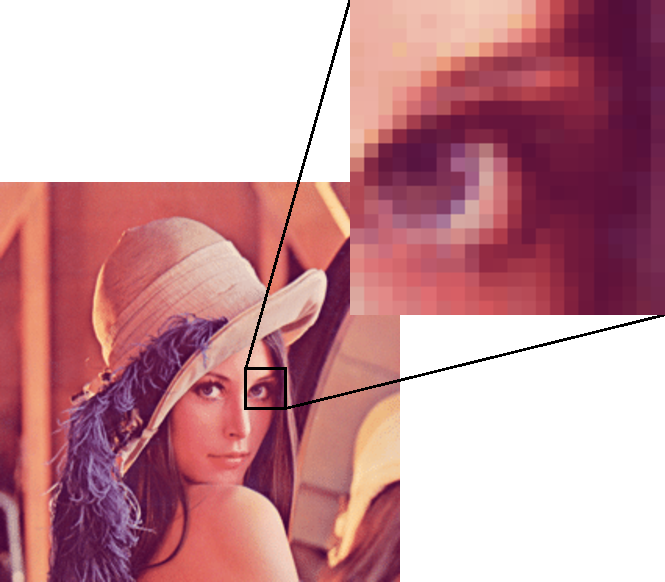
\includegraphics[width=0.5\textwidth]{images/lenaeye.pdf}
  \caption{Lena - detalhe.}\label{fig-lena-detalhe}
  \end{figure}

\end{frame} 

\begin{frame}%[allowframebreaks]
  \frametitle{Espaço necessário para armazenar uma foto}
  \begin{itemize}
  \item câmera 10 Mpixel
  \item 3 bytes por pixel (RGB)
  \item cada foto requer 30 Mbyte
  \item um cartão de memória de 2 Gbytes é capaz de armazenar 66 fotos
  \end{itemize}
\end{frame}

\begin{frame}%[allowframebreaks]
  \frametitle{Espaço necessário para armazenar um vídeo}
  \begin{itemize}
  \item 480 x 720, 30 fps
  \item 345.600 pixels por frame
  \item RGB 3 bytes por pixel
  \item 1.036.800 byte, aprox. 1 Mbyte por frame
  \item 30 frames requerem 31.104.000 bytes, aprox. 31 Mbyte por segundo
  \item um CD de 650 Mbytes é capaz de armazenar apenas 21 segundos de vídeo
  e um DVD de 4.7 GB apenas 155 segundos de vídeo.
  \end{itemize}
\end{frame}


\begin{frame}%[allowframebreaks]
  \frametitle{Dilema de compressão}
  Quando devemos parar a busca por uma \textbf{melhor} compressão?

  \vspace{1cm}
  melhor:
  \begin{itemize}
  \item menor tamanho da representação digital resultante
  \item eficiência computacional (compressão e/ou descompressão)
  \item simplicidade do algoritmo
  \end{itemize}

  \vspace{1cm}
  Qual é o limite de compressão para um determinado dado?

\end{frame} 
\note{
Modificar um algoritmo para melhorar a taxa de compressão em 1\% pode
acarretar um aumento de 10\% no tempo de execução do algoritmo e
ainda mais sobre a complexidade do programa.
}
\note{
Conjecturas\footnote{Uma conjectura é uma proposição que não é provada, mas acredita-se que seja verdadeira e não foi mostrado o contrário.}.
\vspace{2ex}

  \begin{itemize}
  \item Compressão de dados pode ser interpretada como o processo de remover complexidades (redundâncias)
  desnecessárias na informação, e desta forma, maximizando a simplicidade enquanto preserva o máximo
  possível do poder discricionário dos dados.
  \item Todo tipo de computação e racionalização formal pode ser compreendida como compressão
  de informação através do processo de identificar padrões, busca e unificação
  das instâncias destes padrões.
  \end{itemize}

}


\begin{frame}[allowframebreaks]
  \frametitle{Termos}
  \begin{description}
  \item[compressor ou codificador] é o programa que comprime os dados crus na entrada e cria uma saída de dados
  comprimida (com baixa redundância).
  \item[decompressor ou decodificador] converte os dados na direção oposta.
  \item[fluxo] é o dado a ser comprimido, armazenado como um arquivo ou transmitido.
  \item[dado não-codificado, cru, ou original] é o fluxo de dados da entrada.
  \item[dado codificado ou comprimido] é o fluxo de saída.
  \item[método de compressão não-adaptativo] é rígido e não modifica sua operação ou seus parâmetros em resposta
  aos dados em particular que estão sendo comprimidos.
  \item[método adaptativo] analisa os dados crus e modifica sua operação e/ou parâmetros de acordo com os dados em mãos.
  \item[método semi-adaptativo] utiliza 2 passagens aonde, na primeira, realiza a leitura dos dados e
  contabiliza estatísticas dos dados a serem comprimidos; na segunda passagem, realiza de fato a compressão
  utilizados parâmetros determinados na primeira varredura.
  \item[método localmente adaptativo] se adapta às condições locais do fluxo de dados e varia à medida que
  move ao longo dos dados.
  \item[compressão com perdas/sem perdas] : Para atingirem maior compressão, os métodos de compressão com perda
  perdem informação. Os métodos de compressão sem perda não admitem perder informação alguma.
  \item[Compressão em cascata] ocorre quando diferentes métodos de compressão são utilizados um em seguida do outro.
  \item[Compressçao perceptiva] ocorre quando apenas a informação imperceptível pelos nosso sentidos é removida.
  \item[Compressão simétrica] é o caso em que o compressor e descompressor utilizam basicamente o mesmo algoritmo,
  porém em direções opostas.
  \item[Complacente] é o codificador/decodificador que gera/lê de forma correta um fluxo de dados (Qualquer pessoa
  é livre para implementar seu próprio algoritmo).
  \item[Universal] é o método de compressão de dados que não depende da estatística dos dados.
  \item[Razão de Compresão] $=$ tamanho do dado de saída / tamanho do dado de entrada.
  \item[Fator de Compressão] $=$ tamanho do dado de entrada / tamanho do dado de saída $=$ (razão de compressão)$^{-1}$.
  \item[Ganho de Compressão] $= 100 \log_e $ (tamanho de referência / tamanho comprimido), aonde o tamanho de referência é o tamanho dos dados de entrada ou o tamanho do dado de saída comprimido por algum algoritmo padrão.
  \item[Erro médio quadrático (MSE) e relação sinal ruído de sinal (PSNR)] são utilizados para medir a distorção causada por uma compressão com perdas.
  \end{description}
\end{frame} 


\begin{frame}%[allowframebreaks]
  \frametitle{Termos}
  \begin{figure}[h]
  \centering
  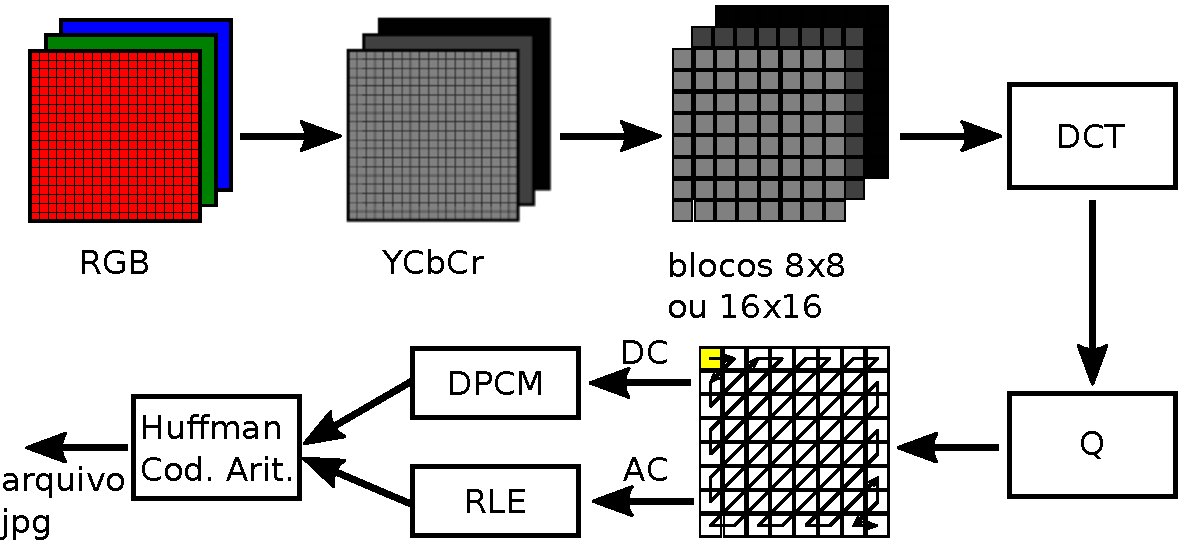
\includegraphics[width=0.8\textwidth]{images/jpegstd.pdf}
  \caption{Esquema de compressão JPEG.}\label{fig-jpegstd}
  \end{figure}
\end{frame} 

\begin{frame}%[allowframebreaks]
  \frametitle{Slides- introdução ao GNU Octave}
  \centering
  
\includegraphics[width=0.4\textwidth]{images/qrcode-octave-intro.pdf}

  \url{https://drive.google.com/open?id=1ew5fl9v_OIybsy3KdEgIvohLTcuwuru_}
\end{frame} 

\begin{frame}%[allowframebreaks]
  \frametitle{Notebook - introdução}
  \centering
  
\includegraphics[width=0.4\textwidth]{images/qrcode-jupyter-intro.pdf}

  \url{https://nbviewer.jupyter.org/github/leolca/notebooks/blob/master/aev/introducao.ipynb}
\end{frame} 

\begin{frame}%[allowframebreaks]
  \frametitle{Notebook - imagem colorida}
  \centering
  
\includegraphics[width=0.4\textwidth]{images/qrcode-jupyter-im-color.pdf}

  \url{https://nbviewer.jupyter.org/github/leolca/notebooks/blob/master/aev/introdocao_imagem_colorida.ipynb}
\end{frame} 



\subsection{Informação}
\begin{frame}%[allowframebreaks]
  \frametitle{Informação}
  O conceito de informação é amplo, sendo difícil ser contemplado em sua plenitude por qualquer definição.

  \vspace{2ex}
  \citet{shannon1948} propôs a definição de \textit{entropia} que possui
  muitas propriedades em comum o senso comum do que deve ser informação.

  \vspace{2ex}
  A informação fornecida por uma mensagem corresponde com o quão improvável é esta mensagem.

\end{frame}
\note{
O que é previsível fornece pouca ou nenhuma informação.

Quanto mais incerto, mais informação há.
}

\begin{frame}%[allowframebreaks]
  \frametitle{Informação}
  \citet{hartley1928} propõem uma medida de informação para uma variável aleatória $X$:
  \begin{equation}
    I(X) = \log_b L ,
  \end{equation}
  onde $L$ é o número de possíveis valores que $X$ pode assumir.
  Se $b=2$, a informação será medida em `bits' (nome sugerido por J.W. Tukey).
\end{frame}
\note{
  A definição de Hartley é condizente com as seguintes intuições sobre informação: 
  \begin{itemize}
  \item Dois cartões de memória devem possuir o dobro da capacidade de um cartão para
  armazenamento de informação.
  \item Dois canais de comunicação idênticos devem possuir o dobro da capacidade 
  de transmitir informação que um único canal.
  \item Um dispositivo com duas posições estáveis, como um relé ou um flip-flop,
  armazena um bit de informação. $N$ dispositivos deste tipo podem armazenar $N$ bits
  de informação, já que o número total de estados é $2^N$ e $\log_2 2^N = N$.
  \end{itemize}

  Entretanto, isto é válido apenas quando as mensagens/eventos são equiprováveis. 
  No caso extremo, note que se o cartão de memória armazena apenas zeros, ele não
  é capaz de armazenar informação alguma.
}

\begin{frame}%[allowframebreaks]
  \frametitle{Entropia}
  Suponha que existam eventos $E_k$ com probabilidade de ocorrência $p_k$. 

  \begin{itemize}
  \item Shannon: informação associada ao evento $E_k$ é dada por $I(E_k) = \log (1/p_k)$.
        \begin{itemize}
        \item Se $p_k=1$ $\rightarrow$ não há surpresa na ocorrência do evento $E_k$.
        \item Se $p_k=0$ $\rightarrow$ surpresa infinita, afinal o evento $E_k$ é impossível.
        \item $I(E_k) = - \log p(E_k)$ é a auto-informação do evento ou mensagem $E_k$.
        \end{itemize}
  \item \textbf{Sempre} utilizaremos a base $2$ para o cálculo do logaritmo, desta forma
  $\log \equiv \log_2$, a menos que seja especificado o contrário.
  \item $\ln$ é o logaritmo na base natural $e$.
  \end{itemize}
\end{frame}

\begin{frame}%[allowframebreaks]
  \frametitle{Entropia}
  \begin{itemize}
  \item Notação: $p(x) = P_X(X=x)$, a probabilidade do evento $\{X=x\}$, da v.a. $X$ assumir o valor $x$.
  \item Valor esperado da v.a. $X$: $E[X] = EX = \sum_x x p(x)$.
  \item Dada uma função $g: \mathcal{X} \rightarrow \mathbb{R}$, o valor esperado da
  v.a. $g(X)$ é $E g(X) = \sum_x g(x) p(x)$.
  \item Considere $g(x) = \log(1/p(x))$. Então $g(x)$ é a imprevisão (surpresa) de encontrar o evento $X=x$.
        Tomando o valor esperado de $g$ teremos
        \begin{equation}
        \sum_x p(x) \log \frac{1}{p(x)} ,
        \end{equation}
        ou seja, a esperança da surpresa, ou o valor esperado da imprevisão na variável aleatória $X$.
        Esta é a definição de entropia.
  \end{itemize}
\end{frame}


% entropia
\section{Entropia}
\subsection{Definição de entropia}
\begin{frame}%[allowframebreaks]
  \frametitle{Entropia}
  \begin{definition}[Entropia]\label{def-entropia}
  Dada uma variável aleatória $X$ sob um alfabeto de tamanho finito $\mathcal{X}$, a \textbf{entropia}
  da variável aleatória é dada por
  \begin{eqnarray}
  H(X) &\triangleq& E_p \log \frac{1}{p(X)} = E \log \frac{1}{p(X)} \\
        &=& \sum_{x \in \mathcal{X}} p(x) \log \frac{1}{p(x)} = - \sum_x p(x) \log p(x)
  \end{eqnarray}
  \end{definition}
  A unidade de entropia é `bits', já que utilizamos o logaritmo na base $2$ (unidade `nats' se 
  utilizar a base $e$).
\end{frame}
\note{  
  \begin{itemize}
  \item Entropia mede a grau de incerteza associado a uma distribuição.
  \item Entropia mede a desordem ou o espalhamento de uma distribuição.
  \item Entropia mede a `escolha' que a fonte tem na escolha de símbolos de acordo com uma densidade 
        (maior entropia implica em mais escolha).
  \item Vamos utilizar a seguinte convenção: $0 \log 0 = 0$.
  \end{itemize}
}

\begin{frame}%[allowframebreaks]
  \frametitle{Entropia}
  Se uma v.a. $X \sim p(x)$, então o valor esperado de uma função desta v.a., $g(X)$, é dada por
  \begin{equation}
  E[g(X)] = \sum_{x \in \mathcal{X}} p(x) g(x) .
  \end{equation}

  A entropia de $X$ pode ser interpretada como o valor esperado da v.a. $\log \frac{1}{p(X)}$,
  onde $X$ é descrita pela função massa de probabilidade $p(x)$.
  \begin{equation}
  H(X) = E \left[ \log \frac{1}{p(X)} \right] .
  \end{equation}
\end{frame}
\note{
  \begin{itemize}
  \item Entropia é uma medida da real `incerteza' média, o que é uma medida sobre toda a distribuição.
  \item Entropia mede o grau de incerteza médio ou esperado do resultado de uma distribuição de probabilidade.
  \item É uma medida de desordem ou espalhamento. Distribuições com alta entropia devem ser planas, mais
  uniformes, enquanto distribuições com baixa entropia devem possuir poucas modas (unimodal, bimodal).
  \end{itemize}
}
\note{
  \begin{figure}[h!]
  \centering
  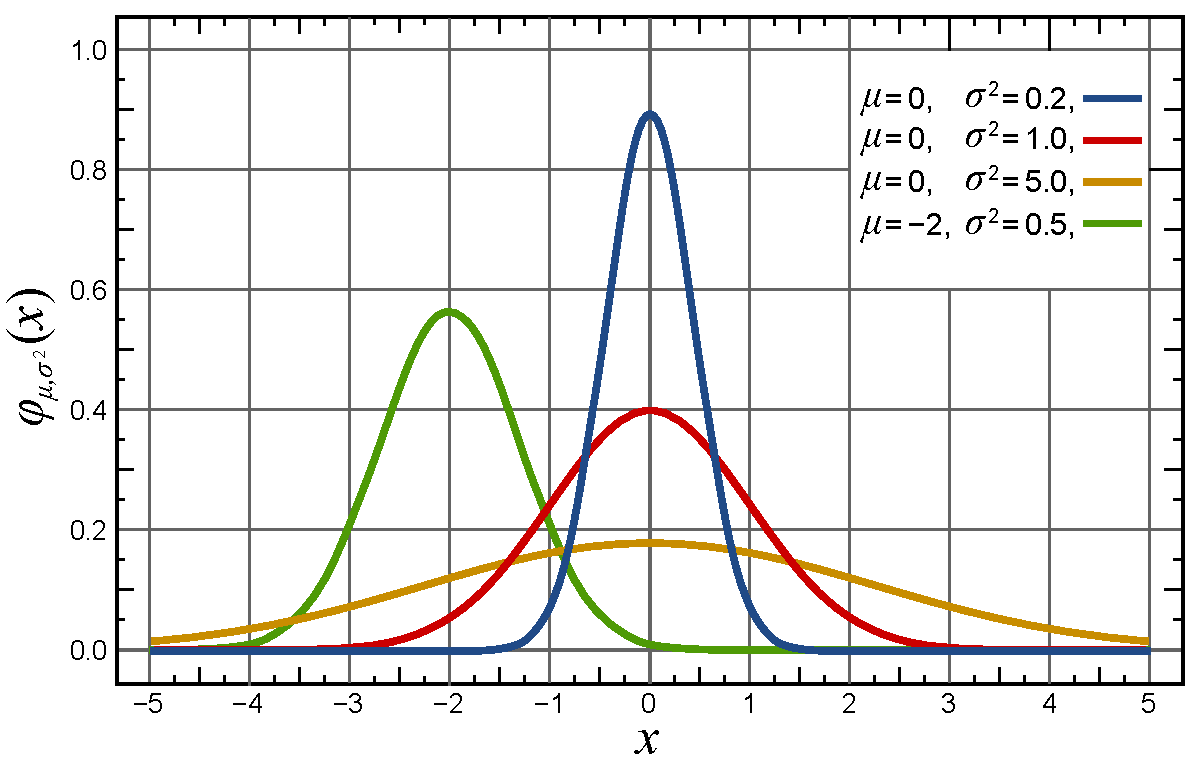
\includegraphics[width=0.4\textwidth]{images/normal_distribution.pdf}
  %\caption{.}
  \label{fig:normal_distribution}
  \end{figure}

  \begin{itemize}
  \item mais concentrado: menor entropia
  \item mais espalhado: maior entropia
  \item os valores em $x$ não importam, 
  apenas os valores das probabilidades associadas $p(x)$ importam no cálculo da entropia
  \end{itemize}
}

\begin{frame}[allowframebreaks]
  \frametitle{Escolha, Incerteza e Entropia}
  Suponha um conjunto de eventos cujas probabilidades de ocorrências sejam dadas
  por $p_1, p_2, \ldots, p_n$. É possível encontrar uma medida de quanta `escolha' 
  está envolvida na seleção de um evento ou quão incertos estamos da saída?

  Para tal medida $H(p_1, p_2, \ldots, p_n)$, é razoável requerermos as seguintes propriedades:
  \begin{enumerate}
  \item $H$ deve ser contínuo em $p_i$;
  \item Se todos os $p_i$ são iguais, $p_i=\frac{1}{n}$, então $H$ deve ser uma função
  monotonicamente crescente de $n$ (quando temos eventos equiprováveis, teremos mais incerteza
  quão maior for o número de eventos possíveis);
  \item Se for possível quebrar uma escolha em uma sequência de escolhas sucessivas,
  a medida $H$ original deve ser a soma ponderada dos valores individuais das medidas
  $H_i$ após a quebra.
  
     \begin{figure}[h!]
     \centering
     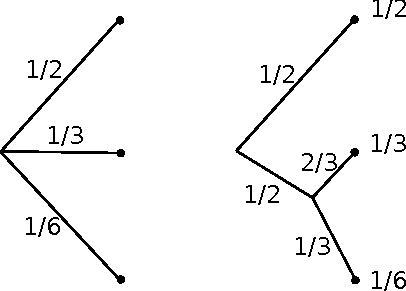
\includegraphics[width=0.3\textwidth]{images/entr-quebra.pdf}
     %\caption{Df.}
     \label{fig:entr-quebra}
     \end{figure}

  \begin{equation}
  H(\frac{1}{2},\frac{1}{3},\frac{1}{6}) = H(\frac{1}{2},\frac{1}{2}) + \frac{1}{2} H(\frac{2}{3},\frac{1}{3})
  \end{equation}
  \end{enumerate}

  A única função $H$ que satisfaz às suposições acima é da forma \cite{shannon1948}: 
  \begin{equation}\label{eq-K-entropia}
  H = - K \sum_{i=1}^{k} p(i) \log p(i) \textmd{ ,}
  \end{equation} 
  onde $K$ é uma constante positiva. 
\end{frame}




\subsection{Demonstração da equação da entropia}
\begin{frame}[allowframebreaks]
  \frametitle{Demonstração da \Cref{eq-K-entropia}}

  Nesta secção iremos apresentar a demonstração de $H=-\sum p_i \log p_i$ 
  (conforme Apêndice 2 de \citet{shannon1948}).

  Vamos definir
  \begin{equation}
  A(n) = H\left( \frac{1}{n}, \frac{1}{n}, \ldots, \frac{1}{n} \right) .
  \end{equation}

  Desejamos que uma escolha dentre $s^m$ opções igualmente prováveis possa ser decomposta como uma sequência de $m$ escolhas
  que se subdividem em $s$ possibilidades igualmente prováveis.

  \begin{figure}[h!]
  \centering
  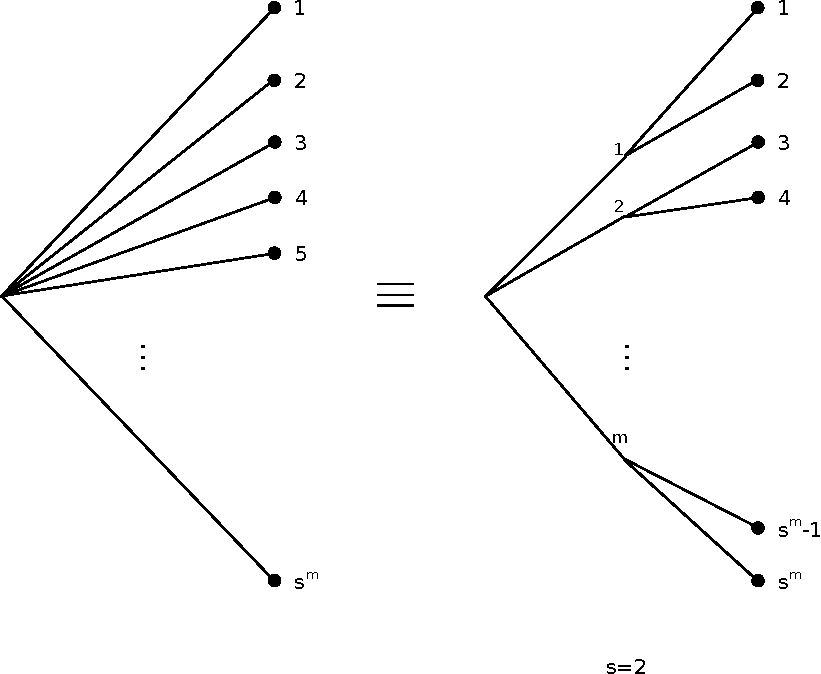
\includegraphics[width=0.5\textwidth]{images/choices.pdf}
  \caption{Exemplo de equivalência para $s=2$.}
  \label{fig:choiceseqv}
  \end{figure}

  Teremos então que
  \begin{equation}
  A(s^m) = m A(s) .
  \end{equation}
  Da mesma forma, para $t$ e $n$, teremos $A(t^n) = n A(t)$.
  Podemos tomar $n$ arbitrariamente grande e encontrar $m$ que satisfaça
  \begin{equation}
  s^m \leq t^n \leq s^{(m+1)} .
  \end{equation}
  Tomando o logaritmo\footnote{Logaritmo é uma função monótona crescente.} da expressão acima e dividindo 
  por $n \log s$ todos os termos\footnote{$n \log s$ é positivo para $n \geq 0$ e $s \geq 1$.}, teremos
  \begin{equation}
  \frac{m}{n} \leq \frac{\log t}{\log s} \leq \frac{m}{n} + \frac{1}{n} ,
  \end{equation}
  o que é equivalente a 
  \begin{equation}
  \left\vert \frac{m}{n} - \frac{\log t}{\log s} \right\vert < \epsilon ,
  \end{equation}
  onde $\epsilon$ é arbitrariamente pequeno, já que $n$ é arbitrariamente grande.

  Usando agora a propriedade desejada de monotonicidade de $A(n)$, teremos
  \begin{alignat}{3}
  A(s^m) &\leq A(t^n) &\leq A(s^{(m+1)}) \nonumber \\
  mA(s) &\leq nA(t) &\leq (m+1)A(s)
  \end{alignat}

  Dividindo a expressão acima por $nA(s)$, teremos
  \begin{equation}
  \frac{m}{n} \leq \frac{A(t)}{A(s)} \leq \frac{m}{n} + \frac{1}{n} ,
  \end{equation}
  ou, de forma equivalente,
  \begin{equation}
  \left\vert \frac{m}{n} - \frac{A(t)}{A(s)} \right\vert < \epsilon ,
  \end{equation}
  e assim, como as duas frações ($\nicefrac{\log t}{\log s}$ e $\nicefrac{A(t)}{A(s)}$) estão $\epsilon$ próximas
  de $\nicefrac{m}{n}$, podemos concluir que
  \begin{equation}
  \left\vert \frac{A(t)}{A(s)} - \frac{\log t}{\log s} \right\vert < 2\epsilon .
  \end{equation}
  Como $\epsilon$ é arbitrariamente pequeno, no limite teremos
  \begin{eqnarray}
  \frac{A(t)}{A(s)} &=& \frac{\log t}{\log s} \nonumber \\
  A(t) &=& \frac{A(s)}{\log s} \log t = K \log t ,
  \end{eqnarray}
  onde $K$ deve ser positivo, de forma que $A(n)$ seja monótona crescente.

  Suponha uma escolha com $n$ possibilidades em que as probabilidades são comensuráveis,
  $p_i = \nicefrac{n_i}{\sum n_i}$, onde $n_i$ são inteiros. De forma equivalente,
  uma escolha entre $\sum n_i$ opções pode ser expressa como uma escolha dentre $n$ opções
  com probabilidades $p_1, \ldots, p_n$, e para uma $i$-ésima dada escolha, realizar uma
  nova escolha dentre $n_i$ opções igualmente prováveis. Teremos então:
  \begin{eqnarray}
  \overbrace{ K \log \left( \sum n_i \right) }^{A\left( \sum n_i \right)} &=& H(p_1, \ldots, p_n) + \overbrace{ K \log n_i }^{A(n_i)} \nonumber \\
  K \underbrace{\left( \sum p_i \right)}_{=1} \log \left( \sum n_i \right) &=& H(p_1, \ldots, p_n) + K \underbrace{\left( \sum p_i \right)}_{=1} \log n_i .
  \end{eqnarray}  
  E assim,
  \begin{eqnarray}
  H(p_1, \ldots, p_n) &=& K\left[ \left( \sum p_i \right) \log \left( \sum n_i \right) - \left( \sum p_i \right) \log n_i \right] \nonumber \\
        &=& -K \sum p_i \log \frac{n_i}{\sum n_i} = -K \sum p_i \log p_i . \qed
  \end{eqnarray} 
\end{frame}



\subsection{Entropia - Fonte Binária}
\begin{frame}%[allowframebreaks]
  \frametitle{Entropia Binária}
  \begin{itemize}
  \item Alfabeto binário $X \in \{0,1\}$, ou $\mathcal{X} = \{0,1\}$.
  \item $p(X=1)=p=1-p(X=0)$.
  \item $H(X) = -p \log p - (1-p) \log (1-p) = H(p)$.
  \item entropia como função de $p$

  \begin{figure}[h!]
  \centering
  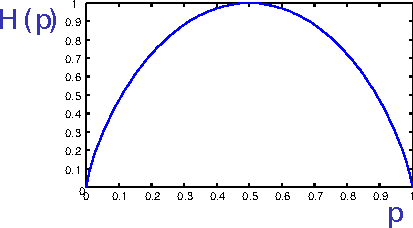
\includegraphics[width=0.5\textwidth]{images/graph_Hp.pdf}
  %\caption{.}
  \label{fig:graph_Hp}
  \end{figure}
  \end{itemize}
\end{frame}
\note{
  \begin{itemize}
  \item maior incerteza ($H=1$) quando $p=0.5$ e menor incerteza ($H=0$) quando $p=0$ ou $p=1$.
  \item note que a entropia $H(p)$ é concava em $p$.
  \end{itemize}
}


\begin{frame}%[allowframebreaks]
  \frametitle{Entropia - GNU Octave}
  \lstinputlisting[firstline=30,lastline=41,label=lst-entropy-fnc]{/home/leoca/ee/research/clscripts/entropy.m}

  \href{https://raw.githubusercontent.com/leolca/clscripts/master/entropy.m}{[download do código]}
\end{frame}

\begin{frame}%[allowframebreaks]
  \frametitle{Entropia - GNU Octave - demo}
  \lstinputlisting[firstline=43,lastline=51,label=lst-entropy-fnc]{/home/leoca/ee/research/clscripts/entropy.m}
\end{frame}

\subsection{Entropia Conjunta}
\begin{frame}%[allowframebreaks]
  \frametitle{Entropia Conjunta}
  Duas variáveis aleatórias $X$ e $Y$ possuem \textbf{entropia conjunta}
  \begin{equation}
  H(X,Y) = - \sum_{x \in \mathcal{X}} \sum_{y \in \mathcal{Y}} p(x,y) \log p(x,y) = E \log \frac{1}{p(X,Y)} .
  \end{equation}

  Generalizando para vetores $X_{1:N} = (X_1, X_2, \ldots, X_N)$
  \begin{eqnarray}
  H(X_{1:N}) &=& H(X_1, X_2, \ldots, X_N) \nonumber \\
       &=& \sum_{x_1, x_2, \ldots , x_N} p(x_1, \ldots, x_N) \log \frac{1}{p(x_1, \ldots, x_N)} \nonumber \\
       &=& E \log \frac{1}{p(X_1, \ldots, X_N)}
  \end{eqnarray}
\end{frame}



\subsection{Entropia Condicional}
\begin{frame}[allowframebreaks]
  \frametitle{Entropia Condicional}
  Dadas duas v.a. $X$ e $Y$ relacionadas por $p(x,y)$, conhecer o evento $X=x$ pode alterar a entropia de $Y$.

  \begin{itemize}
  \item Entropia condicionada a um evento $H(Y|X=x)$
     \begin{eqnarray}
     H(Y|X=x) &=& E \log \frac{1}{p(Y|X=x)} \nonumber \\
              &=& - \sum_{y \in \mathcal{Y}} p(y|x) \log p(y|x)
     \end{eqnarray}

  \item $H(Y|X=x)$ é uma função de $X$. Podemos então tomar seu valor esperado $E[H(Y|X=x)]$
  e obter a entropia condicional $H(Y|X)$.

  \item Realizando a média sobre todos os $x$, obteremos a entropia condicional $H(Y|X)$.
     \begin{eqnarray}
     H(Y|X) &=& \sum_x p(x) H(Y|X=x) \nonumber \\
        &=& - \sum_x p(x) \sum_y p(y|x) \log p(y|x) \nonumber \\
        &=& - \sum_{x,y} p(x,y) \log p(y|x) \nonumber \\
        &=& E \log \frac{1}{p(Y|X)}
     \end{eqnarray}
  \end{itemize}
\end{frame}


\subsection{Regra da Cadeia}
\begin{frame}%[allowframebreaks]
  \frametitle{Regra da Cadeia}
  \begin{theorem}[Regra da Cadeia para a Entropia]
  \begin{equation}
  H(X,Y) = H(X) + H(Y|X) = H(Y) + H(X|Y)
  \end{equation}
  \end{theorem} 
  
  \begin{proof}
  \begin{equation}
  - \log p(x,y) = - \log p(x) - \log p(y|x)
  \end{equation}
  tomando o valor esperado de ambos os lados, obtemos o resultado desejado.
  \end{proof}

  \begin{corollary}
  Se $X \independent Y$ então $H(X,Y) = H(X) + H(Y)$.
  \end{corollary}
\end{frame}


\begin{frame}%[allowframebreaks]
  \frametitle{Regra da Cadeia}
  \begin{proof}[regra da cadeia]
  \begin{eqnarray}
  H(X,Y) &=& - \sum_{x \in \mathcal{X}} \sum_{y \in \mathcal{Y}} p(x,y) \log p(x,y) = - \sum_{x \in \mathcal{X}} \sum_{y \in \mathcal{Y}} p(x,y)  \log p(y|x) p(x) \nonumber \\
        &=& - \sum_{x \in \mathcal{X}} \sum_{y \in \mathcal{Y}} p(x,y)  \log p(y|x) - \sum_{x \in \mathcal{X}} \sum_{y \in \mathcal{Y}} p(x,y)  \log p(x) \nonumber \\
        &=& H(Y|X) - \sum_{x \in \mathcal{X}} \log p(x) \sum_{y \in \mathcal{Y}} p(x,y) \nonumber \\
        &=& H(Y|X) - \sum_{x \in \mathcal{X}} \log p(x) (p(x)) \nonumber \\
        &=& H(Y|X) + H(X)
  \end{eqnarray}
  \end{proof}
\end{frame}
\note{
Exemplo Canal de Comunicação
\vspace{3ex}

   Suponha um canal de comunicação com entrada $X$ e saída $Y$.

   $H(X|Y)$ pode ser visto como a incerteza sobre $X$ (a mensagem enviada) quando 
   $Y$ (a mensagem recebida) for conhecido.

   Sem nenhuma observação no processo de comunicação através deste canal, o
   receptor não sabe nada sobre $X$ nem $Y$, assim a incerteza inicial é $H(X,Y)$.
   Quando o receptor recebe a mensagem $Y$, ele ganha uma quantidade de informação $H(Y)$.
   Assim a informação que falta sobre $X$ mesmo conhecendo $Y$ é dada por
   $H(X|Y) = H(X,Y) - H(Y)$. Esta pode ser tido como uma medida do erro na comunicação.
   A quantidade de informação que o receptor de fato ganha é $I(X;Y) = H(X) - H(X,Y)$.

}

\begin{frame}[allowframebreaks]
  \frametitle{Regra da Cadeia Generalizada}
  \begin{theorem}[Regra da Cadeia para a Entropia]
  \begin{equation}
  H(X_1, X_2, \ldots, X_N) = \sum_{i=1}^N H(X_i | X_1, X_2, \ldots, X_{i-1}) 
  \end{equation}
  \end{theorem}

  \begin{eqnarray}
  H(X_1, X_2, \ldots, X_N) &=& H(X_1) + H(X_2 | X_1) + \\
        && H(X_3 | X_1, X_2) + H(X_4 | X_1, X_2, X_3) + \cdots \nonumber
  \end{eqnarray}
  
  \framebreak
  \begin{proof}
  Utilizando a regra da cadeia da probabilidade condicional, teremos
  \begin{equation}
  p(x_1, x_2, \ldots, x_N) = \prod_{i=1}^N p(x_i | x_1, \ldots , x_{i-1}) ,
  \end{equation}
  então
  \begin{equation}
  - \log p(x_1, x_2, \ldots, x_N) = - \sum_{i=1}^N \log p(x_i | x_1, x_2, \ldots , x_{i-1}) 
  \end{equation}
  tomando o valor esperado de ambos os lados, obtemos o resultado desejado.
  \end{proof}
\end{frame}



\subsection{Propriedades da Entropia}
\begin{frame}%[allowframebreaks]
  \frametitle{Propriedades da Entropia}
  \begin{enumerate}
    \item $H$ é uma função estritamente côncava de $X$, i.e., para $0 \leq \lambda \leq 1$
      e variáveis aleatórias $X$ e $Y$
      \begin{equation}
        H(\lambda X + (1 - \lambda) Y) \geq \lambda H(X) + (1 - \lambda) H(Y)
      \end{equation}
      com igualdade sse (se e somente se) $\lambda = 0$ ou $\lambda = 1$ ou $X=Y$.
    \item $H(X) \geq 0$ com igualdade sse $p(X)$ for não nulo apenas em um ponto $x_0 \in \mathcal{X}$.
    \item $H(X) \leq \log \vert \mathcal{X} \vert$ com igualdade sse $p(X)$ for uniforme ($p \sim \frac{1}{n}$).
    \item $H(X)$ é uma função apenas das probabilidades $p(x_i)$, independente da ordem ou rótulo.
    \item $H_b(X) = (\log_b a) H_a(X)$.
  \end{enumerate}
\end{frame}


\subsection{Continuidade da Entropia}
\begin{frame}[allowframebreaks]
  \frametitle{Continuidade da Entropia}

  Todas as medidas de informação de Shannon são funções contínuas das distribuições
  conjuntas das variáveis aleatórias envolvidas.

  \begin{definition}[distância das variações]
  Seja $p$ e $q$ duas distribuições probabilísticas em um alfabeto comum $\mathcal{X}$.
  A distância das variações entre $p$ e $q$ é definida por
  \begin{equation}
  V(p,q) = \sum_{x \in \mathcal{X}} \vert p(x) - q(x) \vert .
  \end{equation}
  \end{definition} 

  Dado um alfabeto finito fixo $\mathcal{X}$, considere $\mathcal{P}_\mathcal{X}$ o
  conjunto de todas as distribuições em $\mathcal{X}$. A entropia para uma dada distribuição
  $p$ sobre o alfabeto $\mathcal{X}$ é definida por
  \begin{equation}
  H(p) = - \sum_{x \in S_p} p(x) \log p(x) ,
  \end{equation}
  onde $S_p$ denota o suporte de $p$, ou seja, $S_p \subset \mathcal{X}$.
  
  Para que $H(p)$ seja contínuo com respeito à convergência em distância das variações,
  em uma determinada distribuição $p \in \mathcal{P}_\mathcal{X}$, devemos ter que,
  para qualquer $\epsilon > 0$, existe $\delta > 0$ tal que
  \begin{equation}
  \vert H(p) - H(q) \vert < \epsilon ,
  \end{equation}
  para todo $q \in \mathcal{P}_\mathcal{X}$ satisfazendo 
  \begin{equation}
  V(p,q) < \delta ,
  \end{equation}
  ou, de forma equivalente, 
  \begin{equation}
  \lim_{p' \rightarrow p} H(p') = H\left( \lim_{p' \rightarrow p} p' \right) = H(p) ,
  \end{equation}
  onde a convergência $p' \rightarrow p$ é em distância das variações.

  Como $a \log a \rightarrow 0$ quando $a \rightarrow 0$, definimos uma função 
  $l:[0,\infty) \rightarrow \mathbb{R}$ da forma
  \begin{equation}
  l(a) = \begin{cases} 
        a\log a & \quad \text{se } a > 0 , \\
        0       & \quad \text{se } a = 0 ,
        \end{cases}
  \end{equation}
  ou seja, $l(a)$ é uma extensão contínua de $a \log a$.
  Podemos reescrever a entropia da seguinte forma
  \begin{equation}
  H(p) = - \sum_{x \in \mathcal{X}} l(p(x)) ,
  \end{equation}
  onde o somatório é tomado em todo $x \in \mathcal{X}$ ao invés de $S_p$.
  Definindo uma função $l_x: \mathcal{P}_\mathcal{X} \rightarrow \mathbb{R}$, para
  todo $x \in \mathcal{X}$, da forma 
  \begin{equation}
  l_x(p) = l(p(x)) ,
  \end{equation}
  teremos
  \begin{equation}
  H(p) = - \sum_{x \in \mathcal{X}} l_x(p) . \label{eqHsumXl}
  \end{equation}
  Evidentemente $l_x(p)$ é contínua em $p$ (com relação à convergência em 
  distância das variações). Como o somatório na Equação \ref{eqHsumXl} possui
  apenas um número finito de termos, podemos concluir que $H(p)$ é uma função
  contínua de $p$.
\end{frame}


\subsection{Limite Superior da Entropia}
\begin{frame}%[allowframebreaks]
  \frametitle{Limite superior para o Log} 
  \begin{figure}[h!]
  \centering
  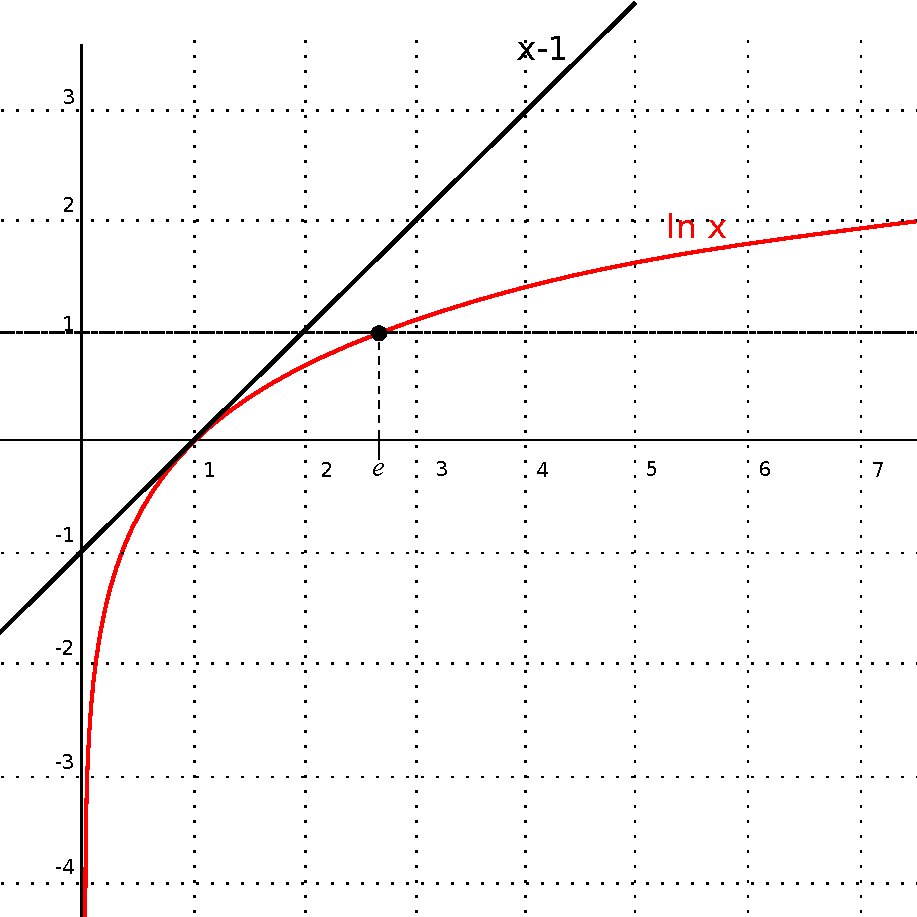
\includegraphics[width=0.4\textwidth]{images/lnx-x-1.pdf}
  %\caption{.}
  \label{fig:lnx-x-1}
  \end{figure}
  \begin{equation}
  \ln x \leq x-1
  \end{equation}
\end{frame}
\note{
$\ln x \leq x-1$, para $x \geq 1$

\begin{itemize}
\item Sabemos que para $x=1$ é verdadeiro, $0 = \ln 1 \leq 1 - 1 =0$.
\item Vamos demonstrar que $\ln x \leq x-1$, para $x \geq 1$ por contradição.
\end{itemize}
Suponha que existe $b > 1$ tal que $\ln x > x - 1$, para $x=b$.
Vamos definir $f(x) = \ln x - x + 1$, logo $f(1) = 0$ (conforme visto acima)
e $f(b) > 0$ (por hipótese).
Pelo teorema do valor médio $\exists c$, $1 < c < b$, tal que
\begin{equation}
f'(c) = \frac{f(b) - f(1)}{b - 1} = \frac{\overbrace{f(b)}^{>0}}{\underbrace{b-1}_{>0}} > 0 .
\end{equation}
Mas, $f'(x) = 1/x -1$, e assim $f'(x) < 0$ para $x>1$. Logo há uma contradição
e nossa hipótese é falsa. Teremos assim $\ln x \leq x-1$, para $x \geq 1$.

Para $x \in (0,1)$, basta seguir os mesmos passos, escolhendo um ponto 
$x=b$, tal que $0 < b < 1$. Vamos encontrar um ponto $c$ tal que $0 < b < c < 1$. 
E usar o teorema do valor médio para mostrar uma contradição na hipótese.  
}


\begin{frame}[allowframebreaks]
  \frametitle{Valor Máximo da Entropia (discreta)}
  \begin{theorem}[Limite Superior da Entropia]
  Seja $X \in \{x_1, x_2, \ldots, x_n\}$. Então $H(X) \leq \log n$, sendo a igualdade
  alcançada se e somente se $p(X=x_i) = \frac{1}{n}$ para todo $i$. 
  \end{theorem}
  \framebreak
  \begin{proof}
  Vamos mostrar que $H(X) - \log n  \leq 0$.
    \begin{eqnarray}
    H(X) - \log n &=& - \sum_x p(x) \log p(x)  - \log n \overbrace{\sum_x p(x)}^{=1} \nonumber \\
        &=& - \sum_x p(x) \log p(x) - \sum_x p(x) \log n \nonumber \\
        &=& - \sum_x p(x) \log p(x) n = \log_2 e \sum_x p(x) \ln \frac{1}{p(x) n} \nonumber \\
        &\leq& \log_2 e \sum_x p(x) \left[ \frac{1}{p(x) n} -1 \right] \nonumber
    \end{eqnarray}

   \proofbreak
    \begin{eqnarray}
    H(X) - \log n &\leq& \ldots \nonumber \\
        &=& \log_2 e \left[ \underbrace{\sum_x \frac{1}{n}}_{\sum_{x \in \mathcal{X}} \frac{1}{n} = n \frac{1}{n} = 1} - \underbrace{\sum_x p(x)}_{=1} \right] = 0
    \end{eqnarray} 
  \end{proof} 
\end{frame}


\begin{frame}%[allowframebreaks]
  \frametitle{Valor Máximo da Entropia}
  Na demonstração acima utilizamos $\ln z \leq z - 1$. A igualdade $\ln z = z-1$ se dará
  no ponto estacionário $z=1$, isto é, quando $\frac{1}{p(x) n} = 1$, ou seja,
  quando $p(x) = 1/n$, teremos assim uma distribuição uniforme.

  \vspace{1cm}
  Se tivermos $p_i = 1/n$, então
  \begin{equation}
  - \sum_i p_i \log p_i = - \sum_i \frac{1}{n} \log \frac{1}{n} = - \log \frac{1}{n} = \log n .
  \end{equation}
  Podemos mostrar (através da concavidade da entropia) que este é o único conjunto de valores com esta propriedade.

  \begin{itemize}
  \item Entropia aumenta quando a distribuição se torna mais uniforme.
  \end{itemize}
\end{frame}

\begin{frame}[allowframebreaks]
  \frametitle{Valor Máximo da Entropia}
  Outra demonstração...

  \begin{proof}
    Considere $X \in \mathcal{X} = \{x_1, x_2, \ldots, x_n\}$ com probabilidades
    $p=\{p_1, p_2, \ldots, p_n\}$, respectivamente. A entropia de $X$ é dada por
    \begin{eqnarray}\label{eq-dem-entr-max2}
    H(X) &=& - \sum_{i=1}^n p_i \log p_i \nonumber \\
        &=& - \sum_{i=1}^{n-1} p_i \log p_i - p_n \log p_n \nonumber \\
        &=& - \left( \frac{1}{\ln 2} \right) \left[ \sum_{i=1}^{n-1} p_i \ln p_i + p_n \ln p_n \right] .
    \end{eqnarray}
    \proofbreak

    Da mesma forma, podemos expressa $p_n$ da seguinte maneira
    \begin{equation}\label{eq-pn-n-1}
    p_n = 1 - \sum_{i=1}^{n-1} p_i .
    \end{equation}
    Utilizando \ref{eq-pn-n-1} em \ref{eq-dem-entr-max2}, podemos expressar
    a entropia $H(X)$ como uma função de $n-1$ probabilidades $p_i$. O máximo
    será dado quando a seguinte condição ocorrer
    \begin{equation}\label{eq:condmaxent}
    \frac{\partial H(X)}{ \partial p_k } = 0 \textmd{ \ for \ } k = 1, \ldots, n-1 \textmd{ .}
    \end{equation}

    \proofbreak
    Teremos então
    \begin{eqnarray}\label{ea:dHeqz}
        0 = \frac{\partial H(X)}{ \partial p_k } &=&  - \left( \frac{1}{\ln 2} \right) \frac{\partial}{ \partial p_k } \left[ \sum_{i=1}^{n-1} p_i \ln p_i  + p_n \ln p_n \right] \nonumber \\
        &=& - \left( \frac{1}{\ln 2} \right) \left[ \ln p_k + 1 + (\ln p_n + 1) \frac{\partial p_n}{ \partial p_k }  \right] \nonumber \\
        &=& - \left( \frac{1}{\ln 2} \right) \left[ \ln p_k + 1 - (\ln p_n + 1) \right] ,
    \end{eqnarray}
    onde utilizamos a Equação \ref{eq-pn-n-1}, que nos fornece $\partial p_n / \partial p_k = -1$.

    \proofbreak
    A Equação \ref{ea:dHeqz} mostra que devemos encontrar $\ln p_k = \ln p_n$ para cada $k=1,\ldots,n-1$.
    Todas as $n-1$ equações serão satisfeitas quando todas as probabilidades $p_k$ forem iguais a $1/n$.

    \proofbreak
    Devemos agora calcular a derivada segunda para mostrar que o extremo que achamos é de fato um máximo.
    \begin{eqnarray}\label{ea:d2Heqz}
        \frac{\partial^2 H(X)}{ \partial p_k^2 } &=& - \left( \frac{1}{\ln 2} \right) \frac{\partial}{ \partial p_k } \left[ \ln p_k - \ln p_n \right] \nonumber \\
           &=& - \left( \frac{1}{\ln 2} \right) \left[ \frac{1}{p_k} + \frac{1}{p_n} \right] \leq 0 \textmd{ ,}
    \end{eqnarray}
    já que as probabilidades são valores positivos. Escolhendo então $p_k = 1/n$, teremos a entropia máxima.

  \end{proof}
\end{frame}



\subsection{Subdividindo em partes}
\begin{frame}[allowframebreaks]
  \frametitle{Subdividindo a entropia em partes}
  A entropia deve permanecer inalterada, mesmo quando subdividimos as escolhas em partes.
 
  \begin{example}[Exemplo simples]
  Suponha uma v.a. $X$ com alfabeto $\mathcal{X} = \{x_1, x_2, x_3, x_4 \}$
  e distribuição $q = (q_1. q_2, q_3, q_4)$.

  A entropia associada a esta variável aleatória é dada por
  \begin{eqnarray}
  H(X) &=& H(q_1, q_2, q_3, q_4) \nonumber \\
        &=& - \sum_{i=1}^{4} q_i \log q_i \nonumber \\
        &=& - q_1 \log q_1 - q_2 \log q_2 - q_3 \log q_3  - q_4 \log q_4 .
  \end{eqnarray}

  \examplebreak

  Se dividirmos a escolha na determinação de $X$ em duas escolhas sucessivas,
  conforme ilustrado na figura abaixo, poderemos então escrever
  \begin{equation}
  H(q_1, q_2, q_3, q_4) = H(p_1, p_2) + p_1 H(p_{1,1}, p_{1,2}) + p_2 H(p_{2,1},p_{2,2}) .
  \end{equation}

        \begin{figure}[h!]
        \centering
        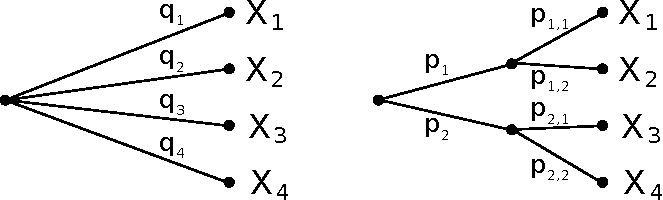
\includegraphics[width=0.5\textwidth]{images/choices4.pdf}
        \label{fig:choices4}
        \end{figure}

  \examplebreak
  \vspace{-2ex}
  \begin{eqnarray}
  H(X)  &=& - q_1 \log q_1 - q_2 \log q_2 - q_3 \log q_3  - q_4 \log q_4 \nonumber \\
        &=& - p_1 p_{1,1} \log p_1 p_{1,1} - p_1 p_{1,2} \log p_1 p_{1,2} - p_2 p_{2,1} \log p_2 p_{2,1} - p_2 p_{2,2} \log p_2 p_{2,2} \nonumber \\
        &=& - p_1 p_{1,1} \log p_1 - p_1 p_{1,1} \log p_{1,1} - p_1 p_{1,2} \log p_1 - p_1 p_{1,2} \log p_{1,2} ... \nonumber \\
        && - p_2 p_{2,1} \log p_2 - p_2 p_{2,1} \log p_{2,1} - p_2 p_{2,2} \log p_2  - p_2 p_{2,2} \log p_{2,2} \nonumber \\
        &=& - p_1 \log p_1 \left( p_{1,1} + p_{1,2} \right) - p_2 \log p_2 \left( p_{2,1} + p_{2,2} \right) ... \nonumber \\
        && + p_1 \left( - p_{1,1} \log p_{1,1} - p_{1,2} \log p_{1,2} \right) ... \nonumber \\
        && + p_2 \left( - p_{2,1} \log p_{2,1} - p_{2,2} \log p_{2,2} \right)  \nonumber \\
        &=& H(p_1, p_2) + p_1 H(p_{1,1}, p_{1,2}) + p_2 H(p_{2,1}, p_{2,2}) 
  \end{eqnarray} 
  \end{example}

  \framebreak

        \begin{figure}[h!]
        \centering
        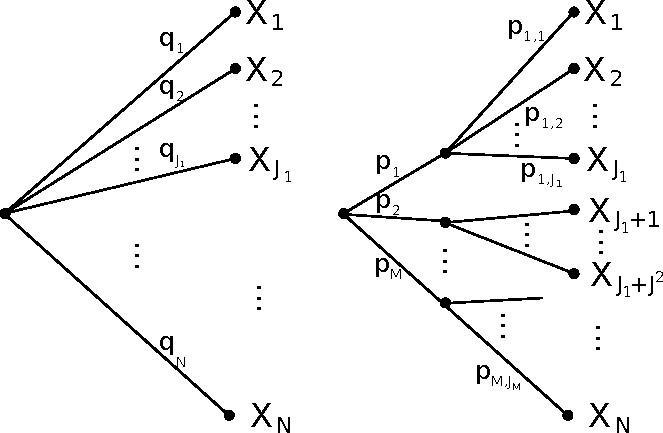
\includegraphics[width=0.5\textwidth]{images/choicesM.pdf}
        \label{fig:choicesM}
        \end{figure} 

  De forma geral, como $q_n = p_m p_{m,j}$, teremos
  \begin{eqnarray}
  H(X) &=& - \sum_{n=1}^N q_n \log q_n = - \sum_{m=1}^M \sum_{j=1}^{J_m} p_m p_{m,j} \log p_m p_{m,j} \nonumber \\
        &=& - \sum_{m=1}^M \sum_{j=1}^{J_m} \left( p_m p_{m,j} \log p_m + p_m p_{m,j} \log p_{m,j} \right) \nonumber \\
        &=& - \sum_{m=1}^M \sum_{j=1}^{J_m} p_m p_{m,j} \log p_m - \sum_{m=1}^M \sum_{j=1}^{J_m} p_m p_{m,j} \log p_{m,j} \nonumber \\
        &=& - \sum_{m=1}^M p_m \log p_m \left( \sum_{j=1}^{J_m} p_{m,j} \right) - \sum_{m=1}^M p_m \sum_{j=1}^{J_m} p_{m,j} \log p_{m,j} \nonumber \\
        &=& H(p_1, \ldots, p_M) + \sum_{m=1}^M p_m H(p_{m,1}, \ldots, p_{m,J_m}) .
  \end{eqnarray}
  
\end{frame}

\subsection{Embaralhar}
\begin{frame}%[allowframebreaks]
  \frametitle{Embaralhar}
  \begin{itemize}
  \item Suponha que $X$ seja uma v.a. indicando as posições de cartas (i.e. $X=x$ representa
  um conjunto de posições, uma determinada configuração).
  \item Seja $T$ uma operação de embaralhamento independente, i.e. $T \independent X$.
  \item Então $H(TX) \geq H(X)$.
  \begin{eqnarray}
  H(TX) &\geq& H(TX|T) \nonumber \\
        && \parbox[c]{0.7\linewidth}{\small onde utilizamos que condicionar não pode aumentar a entropia, como veremos adiante} \nonumber \\
        &=& H(T^{-1}TX|T) \nonumber \\
        && \parbox[c]{0.7\linewidth}{\small como $T$ é conhecido, aplicá-lo novamente ou seu inverso não altera a entropia} \nonumber \\
        &=& H(X|T) = H(X) \\
        && \parbox[c]{0.7\linewidth}{\small onde utilizamos que $T \independent X$} \nonumber
  \end{eqnarray}

%  \begin{equation}
%  H(TX) \geq H(TX|T) = H(T^{-1}TX|T) = H(X|T) = H(X)
%  \end{equation}
%  (onde utilizamos que condicionar não pode aumentar a entropia, como veremos adiante).
  \end{itemize}
\end{frame} 

\begin{frame}%[allowframebreaks]
  \frametitle{Permutação}
  O que ocorre se permutarmos as probabilidades?
  
  Seja $p=(p_1, p_2, \ldots, p_n)$, uma distribuição discreta de probabilidade e
  $\sigma = (\sigma_1, \sigma_2, \ldots, \sigma_n)$ uma permutação de $1, 2, \ldots, n$.
  
  Considere $p_\sigma = (p_{\sigma_1}, p_{\sigma_2}, \ldots, p_{\sigma_n} )$ uma permutação
  da distribuição $p$.

  Quem será maior? $H(p)$ ou $H(p_\sigma)$?

  %\pause
  \begin{equation}
  H(p) = - \sum_i p_i \log p_i = - \sum_j p_{\sigma_j} \log p_{\sigma_j} = H(p_\sigma)  .
  \end{equation}
\end{frame}

\subsection{Sumário}
\begin{frame}%[allowframebreaks]
  \frametitle{Sumário}
  Definição de Entropia
  \begin{equation}
  H(X) = - \sum_x p(x) \log p(x)
  \end{equation}

  Entropia Conjunta
  \begin{equation}
  H(X,Y) = - \sum_{x,y} p(x,y) \log p(x,y)
  \end{equation}

  Entropia Condicional
  \begin{equation}
  H(Y|X) = - \sum_{x,y} p(x,y) \log p(y|x)
  \end{equation}

  Regra da Cadeia
  \begin{equation}
  H(X,Y) = H(X) + H(Y|X) = H(Y) + H(X|Y)
  \end{equation}

  Limites da Entropia
  \begin{equation}
  0 \leq H(X) \leq \log n , \textmd{onde } n \textmd{ é o tamanho do alfabeto de } X.
  \end{equation}

\end{frame}


\subsection{Entropia do Jogo de Adivinhação}

\begin{frame}%[allowframebreaks]
  \frametitle{Entropia do Jogo de Adivinhação}
  Qual é a melhor estratégia para adivinhar o valor de uma variável aleatória
  com perguntas sim/não do tipo ``$X\in S$?'', para algum conjunto $S \subseteq D_X$
  (domínio da v.a. $X$).

  \begin{exampleblock}{Exemplo}
    Seja $X \in D_X = \{x_1, x_2, x_3, x_4, x_5\}$ com probabilidades
        \begin{tabular}{ c | c c c c c}
          $x$    & $x_1$ & $x_2$ & $x_3$ & $x_4$ & $x_5$ \\ \hline
          $p(x)$ & 0.3   & 0.2   & 0.2   & 0.15  & 0.15 \\
        \end{tabular}

    Considere a seguinte estratégia: 
    \begin{inlineenumerate}
        \item $X = x_5$? 
        \item $X = x_4$?
        \item $X = x_3$?
        \item $X = x_2$?
        \item $X = x_1$?
    \end{inlineenumerate}

    Desta forma faremos 5 perguntas 30\% das vezes, 4 perguntas 20\% das vezes, etc.

    O número médio de perguntas é:
    $(0.3, 0.2, 0.2, 0.15, 0.15) \cdot (5,4,3,2,1)^\intercal = 3.35$.

    Se invertermos a ordem das perguntas teremos:
    $(0.3, 0.2, 0.2, 0.15, 0.15) \cdot (1,2,3,4,5)^\intercal = 2.65$.

    Existe uma estratégia melhor?
  \end{exampleblock}
\end{frame}

\begin{frame}%[allowframebreaks]
  \frametitle{Entropia do Jogo de Adivinhação}

  Considere a estratégia ilustrada abaixo.
  \begin{figure}[h!]
  \centering
  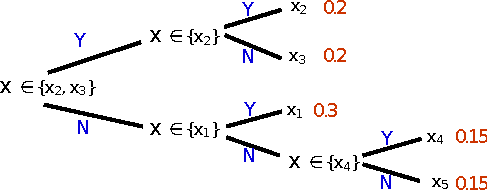
\includegraphics[width=0.75\textwidth]{images/ex-jogo-ad.pdf}
  %\caption{.}
  \label{fig:ex-jogo-ad}
  \end{figure} 

  O número médio de perguntas será:
  $2(0.2 + 0.2 + 0.3) + 3 (0.15 + 0.15) = 2.3$

  Note que $H(X) = 2.271$.

  O número médio de perguntas é sempre $\geq H(X)$.
\end{frame}

\begin{frame}%[allowframebreaks]
  \frametitle{Entropia do Jogo de Adivinhação}
  Vamos analisar a melhor e a pior estratégias, vistas anteriormente,
  com relação à forma como elas dividem a distribuição.

  \begin{itemize}
  \item pior estratégia: $X = x_5$?
 
  Divide a distribuição em dois grupos ($X=x_5$ e $X \neq x_5$), com probabilidades
  $p(X=x_5) = 0.15$, $p(X\neq x_5)=0.85$, e a entropia será $H(0.15 , 0.85) = 0.6098$.

  \item melhor estratégia: $X\in\{x_2,x_3\}$?
  
  $p(X\in\{x_2,x_3\})=0.4$, $p(X\notin\{x_2,x_3\})=0.6$, $H(0.4, 0.6)=0.971$.

  \item De forma geral, é melhor realizar primeiro perguntas que, analisadas como
  variáveis aleatórias, possuem maior entropia (algoritmo guloso).

  \item Note a relação com $H(Y|X) + H(X) = H(X,Y)$. Se fizermos uma pergunta com
  $H(X)$ grande, a entropia residual $H(Y|X)$ fica menor.
  \end{itemize}
\end{frame}
\note{
  Veremos adiante que o algoritmo guloso não é ótimo (entropia mínima).
}




\subsection{Informação Mútua}
\begin{frame}%[allowframebreaks]
  \frametitle{Intuição sobre Informação Mútua}
  \begin{itemize}
  \item Dadas duas variáveis aleatórias $X$ e $Y$, quanta informação uma possui sobre a outra?
  \item Conhecendo $X$, quanto sabemos sobre $Y$? Conhecendo $Y$, quanto sabemos sobre $X$?
  \item Se as v.a.s são independentes, $X \independent Y$, então conhecer $X$ não nos diz nada sobre
  $Y$ e vice-versa.
  \item Como temos uma medida de informação em uma fonte aleatória, $H(X)$, podemos quantificar
  quanta informação variáveis aleatórias possuem uma sobre as outras. Isto é chamado de 
  \underline{informação mútua}.
  \end{itemize}
\end{frame}

\begin{frame}%[allowframebreaks]
  \frametitle{Informação Mútua de Evento}
  Dado o evento $\{X=x, Y=y\}$, podemos nos perguntar sobre qual é a informação fornecida
  pelo evento $x$ dado o fato de que o evento $y$ ocorreu. Isto pode ser quantificado da seguinte forma:
  \begin{equation}
  I(x;y) = \log \frac{p(x|y)}{p(x)} = \underbrace{\log \frac{1}{p(x)}}_{A} - \underbrace{\log \frac{1}{p(x|y)}}_{B}
  \end{equation}
  
  \begin{itemize}
  \item Primeiro termo $A$: surpresa de que $x$ ocorreu.
  \item Segundo termo $B$: surpresa de que $x$ ocorreu dado que $y$ ocorreu.
  \item Diferença: diferença entre as duas surpresas, quanto mudou na surpresa de quando
  não sabíamos $y$ para quando passamos a saber $y$.
  \end{itemize}

  Note que $p(x|x)=1$, então $I(x;x) = \log 1/p(x) - \log 1 = \log 1/p(x) = I(x)$, então
  $I(x)$ pode ser visto como uma forma de `auto-informação'.
\end{frame}

\begin{frame}%[allowframebreaks]
  \frametitle{Informação Mútua}
  Informação Mútua é a quantidade média de informação que uma variável aleatória 
  $X$ possui sobre outra v.a. $Y$ e vice-versa.

  \begin{definition}[Informação Mútua]\label{def-inf-mut}
    \begin{eqnarray}
    I(X;Y) &=& E_{p(x,y)} \log \frac{p(x|y)}{p(x)} = E_{p(x,y)} \log \frac{p(x|y)p(y)}{p(x)p(y)} \nonumber \\
        &=& E_{p(x,y)} \log \frac{p(x,y)}{p(x)p(y)} = \sum_{x,y} p(x,y) \log \frac{p(x,y)}{p(x)p(y)}
    \end{eqnarray}
  \end{definition}
\end{frame}

\begin{frame}%[allowframebreaks]
  \frametitle{Informação Mútua e Entropia}
  \begin{proposition}
    \begin{equation}
        I(X;Y) = H(X) - H(X|Y)
    \end{equation}
  \end{proposition}
  \begin{proof}
    \vspace{-0.3cm}
    \begin{eqnarray} 
        I(X;Y)  &=& E \log \frac{p(x|y)}{p(x)} \nonumber \\
                &=& E \log \frac{1}{p(x)} - E \log \frac{1}{p(x|y)} \nonumber \\
                &=& H(X) - H(X|Y)
    \end{eqnarray}
  \end{proof}

  \begin{itemize}
  \item Por simetria, temos que $I(X;Y) = H(Y) - H(Y|X)$.
  \item Como $H(X) \geq 0$ e $H(X|Y) \geq 0$, teremos $I(X;Y) \leq \min (H(X),H(Y))$.
  \end{itemize}
\end{frame}

\begin{frame}%[allowframebreaks]
  \frametitle{Informação Mútua e Entropia}
  \begin{itemize}
  \item Regra da Cadeia da Entropia: $H(X,Y) = H(X) + H(Y|X)$.
  \item Informação Mútua: $I(X;Y) = H(X) - H(X|Y)$.
  \item Teremos então: 
        \begin{equation}
        I(X;Y) = H(X) + H(Y) - H(X,Y)
        \end{equation}
  \end{itemize}

   No próximo slide representamos estas grandezas através de um diagrama.
   As áreas utilizadas não representam conjuntos no sentido comum, mas
   representam `grau de informação' e as intersecções correspondem a
   sobreposição de informação. Isto é, a interseção consiste em informação
   fornecida por $X$ e $Y$.
\end{frame}

\begin{frame}%[allowframebreaks]
  \frametitle{Informação Mútua e Entropia - Diagrama}

  \begin{figure}[h!]
  \centering
  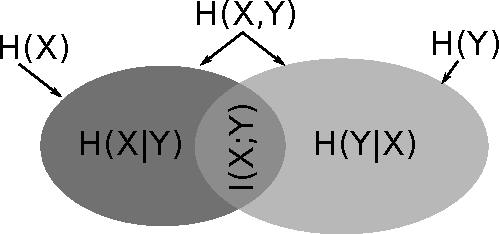
\includegraphics[width=0.75\textwidth]{images/info-set.pdf}
  %\caption{.}
  \label{fig:info-set}
  \end{figure}

\end{frame}

\subsection{Divergência de Kullbach-Leibler}
\begin{frame}%[allowframebreaks]
  \frametitle{Divergência de Kullbach-Leibler}
  A divergência de Kullbach-Leibler é uma relação fundamental entre duas 
  distribuições probabilísticas sobre um mesmo alfabeto, $p=(p_1, \ldots, p_n)$
  e $q=(q_1, \ldots , q_n)$. Esta divergência possui relação importante com a
  entropia e a informação mútua. 

  \vspace{1cm}
  Como podemos medir a `distância' entre duas distribuições $p$ e $q$ de forma útil?
  Poderíamos utilizar $D(p,q) = \sum_{i=1}^n (p_i - q_i)^2$, mas gostaríamos de ter
  uma medida de `distância de informação', isto é, uma distância que nos dê o custo
  incorrido pelo erro de considerar que uma distribuição é $q$ sendo que na realidade
  ela é $p$. Veremos que isto está ligado à insuficiência na compressão. 
  A Divergência de Kullbach-Leibler, definida a seguir, satisfaz estas ideias.
\end{frame}

\begin{frame}[allowframebreaks]
  \frametitle{Distância}
  \begin{definition}[distância]
  Seja $S$ um conjunto. Uma função $d: S \times S \rightarrow \mathbb{R}$ é chamada \textbf{distância} em $S$
  se, para todo $x,y \in S$, tivermos:
  \begin{itemize}
  \item $d(x,y) \geq 0$ (não-negatividade)
  \item $d(x,y) = d(y,x)$ (simetria)
  \item $d(x,x) = 0$ (reflexividade)
  \end{itemize}
  \end{definition}

  \framebreak
  \begin{definition}[métrica]
  Seja $S$ um conjunto. Uma função $d: S \times S \rightarrow \mathbb{R}$ é chamada \textbf{métrica} em $S$
  se, para todo $x,y \in S$, tivermos:
  \begin{itemize}
  \item $d(x,y) \geq 0$ (não-negatividade)
  \item $d(x,y) = 0$ se e somente se $x=y$ (identidade dos indiscerníveis)
  \item $d(x,y) = d(y,x)$ (simetria)
  \item $d(x,y) + d(y,z) \geq d(x,z)$ (desigualdade triangular)
  \end{itemize}
  \end{definition}
\end{frame}
\note{
Teremos uma semi-métrica se substituirmos a identidade dos indiscerníveis pela reflexividade.
}

\begin{frame}%[allowframebreaks]
  \frametitle{Diferentes formas de medir `distância' entre distribuições}

  \begin{description}
  \item[divergência de Kullback-Leibler:] $D_\mathrm{KL}(p \parallel q) = \sum p(x)\ln\left( \frac{p(x)}{q(x)}\right) $;
  \item[distância de Hellinger:] $H^2(p,\, q) = 2 \sum \Big( \sqrt{p(x)} - \sqrt{q(x)}\, \Big)^2 $;
  \item[divergência de Jeffreys:] $D_J(p \parallel q) = \sum (p(x) - q(x))\big( \ln p(x) - \ln q(x) \big) $;
  \item[divergência $\alpha$ de Chernoff:] $D^{(\alpha)}(p \parallel q) = \frac{4}{1-\alpha^2}\bigg(1 - \sum p(x)^\frac{1-\alpha}{2} q(x)^\frac{1+\alpha}{2}  \bigg) $;
  \item[divergência exponencial:] $D_e(p \parallel q) = \sum p(x)\big( \ln p(x) - \ln q(x) \big)^2$;
  \item[divergência de Kagan:] $D_{\chi^2}(p \parallel q) = \frac12 \sum \frac{(p(x) - q(x))^2}{p(x)}$;
  \item[divergência K:] $D_{\mathrm{K}}(p \parallel q) = \sum (p(x) - q(x)) \log(p(x)/q(x))$;
  \item[divergência de Jensen-Shannon:] $D_{\mathrm{JS}}(p \parallel q) = \tfrac{1}{2} D_{\mathrm{KL}} \left (p \parallel m \right ) + \tfrac{1}{2} D_{\mathrm{KL}}\left (q \parallel m \right )\, \!$, onde $m = \tfrac{1}{2}(p+q)$.
  \end{description}
\end{frame}

\begin{frame}%[allowframebreaks]
  \frametitle{Divergência de Kullbach-Leibler (Entropia relativa)}
  Sejam dadas duas distribuições, $p(x)$ e $q(x)$ sobre o mesmo alfabeto,
  $p(x) = P_p (X=x)$ e $q(x) = P_q (X=x)$, a divergência de KL é definida por

  \begin{definition}[Divergência de Kullbach-Leibler (entropia relativa)]
  \begin{equation}
  D(p||q) \triangleq \sum_x p(x) \log \frac{p(x)}{q(x)}
  \end{equation}
  \end{definition}
  Esta divergência pode ser vista como o valor esperado do logaritmo da razão das possibilidades, 
  ponderado por $p$, ou seja, $E_p \log p/q$, ou ainda, o valor esperado da diferença dos 
  logaritmos, $D(p||q) = E_p \left( \log p(x) - \log q(x) \right)$. Fornece a ideia do custo adicional
  (em bits) em se considerar uma distribuição $q$ quando a real distribuição subjacente é $p$.

  Note que a divergência de KL, em geral, não é simétrica, ou seja,
  $D(p||q) \neq D(q||p)$.

\end{frame}
\note{
  Utilizando argumentos de limite e continuidade, mostra-se que $0 \log 0 = 0$
  e $p \log (p/0) = \infty$. Fazendo estas suposições, teremos
  $D(p||q) \leq \infty$.

  A divergência de KL é uma função dos valores de probabilidade e não dos
  valores que a variável aleatória assume (assim como a entropia e a informação mútua).

  \vspace{3em}

A razão de chances ou razão de possibilidades (em inglês: \textit{odds ratio})
é definida como a razão entre a chance de um evento ocorrer em um grupo e a chance de ocorrer em outro grupo.
}
\note{
(Wikipedia)
In statistics, the odds ratio (usually abbreviated "OR") is one of three main ways 
to quantify how strongly the presence or absence of property A is associated with 
the presence or absence of property B in a given population. If each individual in 
a population either does or does not have a property "A", (e.g. "high blood pressure"), 
and also either does or does not have a property "B" (e.g. "moderate alcohol consumption") 
where both properties are appropriately defined, then a ratio can be formed which 
quantitatively describes the association between the presence/absence of "A" 
(high blood pressure) and the presence/absence of "B" (moderate alcohol consumption) 
for individuals in the population. 
}
\note{
This ratio is the odds ratio (OR) and can be computed 
following these steps:
\begin{enumerate}
\item For a given individual that has "B" compute the odds that the same individual has "A"
\item For a given individual that does not have "B" compute the odds that the same individual has "A"
\item Divide the odds from step 1 by the odds from step 2 to obtain the odds ratio (OR).
The term "individual" in this usage does not have to refer to a human being, as 
a statistical population can measure any set of entities, whether living or inanimate.
\end{enumerate}
\url{http://en.wikipedia.org/wiki/Odds_ratio}
}

\begin{frame}%[allowframebreaks]
  \frametitle{Exemplo}
  Seja $\mathcal{X} = \{1,0\}$ e considere duas distribuições $p$ e $q$ em $\mathcal{X}$.
  Seja $p(0)=1-r$, $p(1)=r$, e seja $q(0)=1-s$ e $q(1)=s$. Então
  \begin{equation}
  D(p||q) = (1-r) \log \frac{1-r}{1-s} + r \log \frac{r}{s}
  \end{equation}
  e
  \begin{equation}
  D(q||p) = (1-s) \log \frac{1-s}{1-r} + s \log \frac{s}{r} .
  \end{equation}
  Se $r=s$, então $D(p||q)=D(q||p)=0$. Se $r=\frac{1}{2}$ e $s=\frac{1}{4}$, 
  \begin{equation}
  D(p||q) = \frac{1}{2} \log \frac{1/2}{3/4} + \frac{1}{2} \log \frac{1/2}{1/4} = 1 - \frac{1}{2} \log 3 = 0.2075 \text{bits.}
  \end{equation}
  \begin{equation}
  D(q||p) = \frac{3}{4} \log \frac{3/4}{1/2} + \frac{1}{4} \log \frac{1/4}{1/2} = \frac{3}{4} \log 3 - 1 = 0.1887 \text{bits.}
  \end{equation}

   Note que, em geral, $D(p||q) \neq D(q||p)$.
\end{frame}

\begin{frame}%[allowframebreaks]
  \frametitle{Generalização da divergência de KL}
  A divergência de KL pode ser generalizada para vetores de variáveis aleatórias.

  Seja $p(x_1, \ldots, x_N)$ e $q(x_1, \ldots, x_N)$ duas distribuições sobre o vetor
  $(x_1, x_2, \ldots , x_N)$. A divergência de KL entre $p$ e $q$ é definida por
  \begin{equation}
  D(p||q) = \sum_{x_1, \ldots, x_N} p(x_1, \ldots, x_N) \log \frac{p(x_1, \ldots, x_N)}{q(x_1, \ldots, x_N)}
  \end{equation}
\end{frame}

\begin{frame}[allowframebreaks]
  \frametitle{Divergência de KL e Informação Mútua}
  Seja $\mu_1(x,y) = p(x,y)$ (distribuição conjunta) e $\mu_2(x,y)=p(x)p(y)$ (produto das marginais) 
  com $p(x)=\sum_y p(x,y)$ e $p(y)=\sum_x p(x,y)$, então
  \begin{eqnarray}
  D(\mu_1 || \mu_2) &=& \sum_{x,y} \mu_1(x,y) \log \frac{\mu_1(x,y)}{\mu_2(x,y)} \nonumber \\
                &=& \sum_{x,y} p(x,y) \log \frac{p(x,y)}{p(x)p(y)} = I(X;Y) .
  \end{eqnarray}
  A informação mútua é a distância entre a distribuição conjunta em $X$ e $Y$ e o produto
  das distribuições marginais em $X$ e $Y$.

  Se as v.a.s são independentes, teremos $p(x,y)=p(x)p(y)$ e por conseguinte a divergência será nula,
  a informação mútua entre $X$ e $Y$ será zero.

  A informação mútua é o erro em se assumir independência entre as v.a.s.

  \framebreak
  O produto das distribuições marginais $p(x)p(y)$, onde $p(x)=\sum_y p(x,y)$ e $p(y)=\sum_x p(x,y)$,
  é uma projeção da distribuição conjunta $p(x,y)$ sobre o conjunto das distribuições independentes.
  I.e.,
  \begin{equation}
  p(x)p(y) = \argmin_{p'(x,y) \backslash p'(x,y)=p'(x)p'(y)} D(p(x,y)||p'(x,y)) 
  \end{equation}
\end{frame}


\begin{frame}[allowframebreaks]
  \frametitle{Minimizar a Divergência de KL equivale a maximizar o logaritmo da verossimilhança}
  Suponha que tenhamos uma v.a. $\mathbf{X}=(X_1,\ldots,X_N)$ com uma distribuição subjacente $p$
  que depende de um parâmetro $\theta$ (modelo hipotético). Queremos definir um estimador 
  $\hat{\theta} = T(X_1, \ldots, X_N)$ para este parâmetro $\theta$, dadas as observações $x_1, \ldots, x_N$.
  Um bom estimador para o parâmetro desconhecido $\theta$ é aquela que maximiza a verossimilhança $L(\theta)$ 
  do parâmetro, dada a observação dos dados,
  \begin{equation}
  L(\theta) = \Pr(X_1=x_1, \ldots, X_N=x_N) = p(x_1|\theta) \ldots p(x_N|\theta) = \prod_{n=1}^{N} p(x_n|\theta) .
  \end{equation}
  Como a função logaritmo é monotônica crescente, maximizar $L(\theta)$ é equivalente a maximiza $l(\theta) = \log L(\theta)$,
  \begin{equation} 
  \ell(\theta) = \sum_{n=1}^{N} \log p(x_n|\theta) .
  \end{equation}

  A estimativa de máxima verossimilhança (MLE, \textit{maximum likelihood estimator}) de $\theta$ é dada por
  \begin{equation}
  \hat\theta_\mathrm{mle} = \argmax_{\theta\in\Theta} \ell(\theta\,;\,x_1,\ldots,x_N) .
  \end{equation}

  \framebreak

  Chamaremos de $\hat{p}$ a distribuição empírica. Seja $x_1, \ldots, x_N \in \mathcal{X}$, $N$ observações
  i.i.d. de uma variável aleatória $X$. A distribuição empírica será dada por
  \begin{equation}
  \hat{p}(x) = \frac{1}{N} \sum_{n=1}^{N} \delta(x - x_n) ,
  \end{equation}
  onde $\delta$ é a função de Dirac.

  \vspace{3em}
  Seja $p_\theta$ uma distribuição em $\mathcal{X}$ parametrizada por $\theta$. 
  Maximizar a verossimilhança de $p_\theta(x)$ é equivalente a minimizar a divergência de KL 
  $D_\mathrm{KL}(\hat{p} \parallel p_\theta)$.

  \framebreak

  \begin{eqnarray}
  D_\mathrm{KL}(\hat{p} \parallel p_\theta) &=& \sum_{x \in \mathcal{X}} \hat{p}(x) \log \frac{\hat{p}(x)}{p_\theta(x)} \nonumber \\
        &=& -H(\hat{p}) - \sum_{x \in \mathcal{X}} \hat{p}(x) \log p_\theta(x)  \nonumber \\
        &=& -H(\hat{p}) - \frac{1}{N} \sum_{x \in \mathcal{X}} \sum_{n=1}^{N} \delta(x - x_n) \log p_\theta(x) \nonumber \\
        &=& -H(\hat{p}) - \frac{1}{N} \sum_{n=1}^{N} \log p_\theta(x_n) .
  \end{eqnarray}
  O segundo termo é o oposto do logaritmo da verossimilhança de $p_\theta(x)$.
  
  \framebreak

  A estimativa máxima verossimilhança de $\theta$ a partir das $N$ observações é dada por
  \begin{eqnarray}
  \hat{\theta}_n &=& \argmax_{\theta \in \Theta} \prod_{n=1}^{N} p_\theta(x_n) \nonumber \\
	    &=& \argmax_{\theta \in \Theta} \sum_{n=1}^{N} \log p_\theta(x_n) \nonumber \\
        &=& \argmin_{\theta \in \Theta} \frac{1}{N} \sum_{n=1}^{N} - \log p_\theta(x_n) .
  \end{eqnarray}
   Desta forma, podemos constatar que a distribuição que minimiza a divergência de KL para a distribuição empírica é
   aquela que maximiza a verossimilhança (ou logaritmo desta).
  
%  Pela lei forte dos grandes números, $\frac{1}{N} \sum_{i=1}^{N} \log p_\theta(x_n) \xrightarrow{q.c.} \E[ \log p_\theta(X) ]$.

\end{frame}
% https://www.cs.ubc.ca/~murphyk/Teaching/CS340-Fall06/reading/infoTheory.pdf
% https://www.di.ens.fr/~fbach/courses/fall2013/lecture5.pdf
% http://nowak.ece.wisc.edu/SLT09/lecture13.pdf


\subsection{Informação Mútua Condicional}
\begin{frame}%[allowframebreaks]
  \frametitle{Informação Mútua Condicionada a um evento}
  A informação pode se alterar se for condicionada a um evento de uma terceira variável
  aleatória $\{Z=z\}$, e isto é denotado por $I(X;Y|Z=z)$, onde $X,Y,Z$ são variáveis
  aleatórias.

  Dada a distribuição $p(x,y,z)$, a informação mútua condicionada ao evento específico
  $\{Z=z\}$ é dada por
  \begin{equation}
  I(X;Y|Z=z) = \sum_{x,y} p(x,y|z) \log \frac{p(x,y|z)}{p(x|z)p(y|z)} .
  \end{equation}

  Obs. Fazemos as seguintes alterações sobre a informação mútua padrão: 
  $p(x,y)\rightarrow p(x,y|z)$, $p(x)\rightarrow p(x|z)$ e $p(y) \rightarrow p(y|z)$.
\end{frame}

\begin{frame}%[allowframebreaks]
  \frametitle{Informação Mútua Condicional}
   A informação entre duas variáveis aleatórias pode mudar na média se for condicionada 
   a uma terceira variável aleatória. Será denotada por $I(X;Y|Z)$.
   \begin{definition}[Informação Mútua Condicional]
   \vspace{-0.3cm}
   \begin{eqnarray}
     I(X;Y|Z) &\triangleq& \sum_z p(z) I(X;Y|Z=z) \nonumber \\
                &=& \sum_z p(z) E_{p(x,y|z)} \log \frac{p(x,y|Z=z)}{p(x|Z=z) p(y|Z=z)} \nonumber \\
                &=& \sum_{x,y,z} p(x,y,z) \log \frac{p(x,y|z)}{p(x|z)p(y|z)} \nonumber \\
                &=& E \left[ \log \frac{1}{p(x|z)} - \log \frac{1}{p(x|y,z)} \right] \nonumber \\
                &=& H(X|Z) - H(X|Y,Z)
   \end{eqnarray}
   \end{definition}
\end{frame}
\note{
\begin{equation}
 I(X;Y) = H(X) - H(X|Y)
\end{equation}

\begin{equation}
 I(X;Y|Z) = H(X|Z) - H(X|Y,Z)
\end{equation}
}



\subsection{Propriedades da Informação Mútua}
\begin{frame}%[allowframebreaks]
  \frametitle{Regra da Cadeia para Informação Mútua}
   \begin{proposition} \vspace{-0.2cm}
   \begin{equation}
   I(X_1,X_2,\ldots,X_N;Y) = \sum_i I(X_i;Y|X_1,X_2,\ldots,X_{i-1})
   \end{equation}
   \end{proposition}
   
   Exemplo: $I(X_1,X_2;Y) = I(X_1;Y) + I(X_2;Y|X_1)$
   \begin{proof} \vspace{-0.6cm}
   \begin{eqnarray}
        I(X_1,\ldots,X_N;Y) &=& H(X_1,\ldots,X_N) - H(X_1,\ldots,X_N|Y) \nonumber \\
                &=& \sum_{i=1}^N H(X_i|X_1,\ldots,X_{i-1}) - \sum_{i=1}^N H(X_i|X_1,\ldots,X_{i-1},Y) \nonumber \\
                &=& \sum_{i=1}^N I(X_i;Y|X_1,\ldots,X_{i-1}) 
   \end{eqnarray}
   \end{proof}
\end{frame}

\begin{frame}%[allowframebreaks]
  \frametitle{Entropia Relativa Condicional - divergência de KL}
  \begin{definition}
  Para pmf conjuntas $p(x,y)$ e $q(x,y)$, a entropia relativa condicional é definida como
  \begin{eqnarray}
        D(p(y|x) || q(y|x)) &\triangleq& \sum_x p(x) \sum_y p(y|x) \log \frac{p(y|x)}{q(y|x)} \nonumber \\
                &=& \sum_{x,y} p(x,y) \log \frac{p(y|x)}{q(y|x)} \nonumber \\
                &=& \E_{p(x,y)} \log \frac{p(Y|X)}{q(Y|X)} ,
  \end{eqnarray}
  é o valor esperado das entropias relativas entre as pmfs condicionais $p(y|x)$ e $q(y|x)$, 
  tomando o valor esperado sobre a distribuição de massa $p(x)$.
  \end{definition} 
\end{frame}


\begin{frame}%[allowframebreaks]
  \frametitle{Regra da Cadeia para divergência de KL}
  \begin{proposition}
  \begin{equation}
  D(p(x,y)||q(x,y)) = D(p(x)||q(x)) + D(p(y|x)||q(y|x))
  \end{equation}
  \end{proposition}

  \begin{proof}
  \begin{eqnarray}
  D(p(x,y)||q(x,y)) &=& \sum_{x,y} p(x,y) \log \frac{p(x,y)}{q(x,y)} = \sum_{x,y} p(x,y) \log \frac{ p(y|x)p(x) }{ q(y|x)q(x) } \nonumber \\
        &=& \sum_{x,y} p(x,y) \log \frac{ p(y|x) }{ q(y|x) } + \sum_{x,y} p(x,y) \log \frac{ p(x) }{ q(x) } 
  \end{eqnarray}
  \end{proof}
\end{frame}



\subsection{Desigualdade de Jensen}
\begin{frame}%[allowframebreaks]
  \frametitle{Funções Convexas}
   \begin{definition}
   Dizemos que $f$ é convexa em $(a,b)$ se para todo $x_1,x_2 \in (a,b)$, $0 \leq \lambda \leq 1$,
   \begin{equation}
   f(\lambda x_1 + (1 - \lambda)x_2) \leq \lambda f(x_1) + (1-\lambda) f(x_2)
   \end{equation}
   \end{definition}
   Exemplos:  
    \begin{inlineenumerate}
        \item $f(x)=x^2$
        \item $f(x)=e^x$
        \item $x \log x$, $x \geq 0$.
    \end{inlineenumerate}
  \begin{figure}[h!]
  \centering
  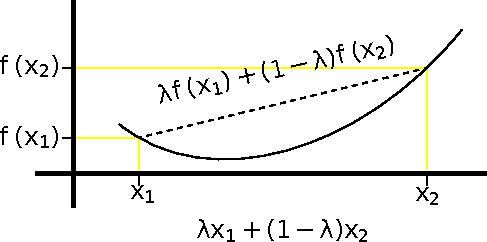
\includegraphics[width=0.5\textwidth]{images/funcao-convexa.pdf}
  %\caption{.}
  \label{fig:funcao-convexa}
  \end{figure}
  \begin{itemize}
  \item $f$ é estritamente convexa se a igualdade for verdadeira 
  apenas para $\lambda = 0$ ou $\lambda = 1$.
  \end{itemize}
\end{frame}

\begin{frame}[allowframebreaks]
  \frametitle{Derivada Segunda e Convexidade}
  \begin{theorem}[derivada segunda e convexidade]
  Se uma função $f$ possui derivada segunda não-negativa (positiva) em um intervalo,
  a função é convexa (estritamente convexa) no intervalo.
  \end{theorem}

  \begin{proof}
  A expansão de Taylor de uma função $f$ em torno do ponto $x_0$ é dada por
  \begin{equation}
  f(x) = f(x_0) + f'(x_0) (x-x_0) + \frac{f''(x^\ast)}{2} (x-x_0)^2
  \end{equation}
  onde $x^\ast \in (x_0,x)$. Por hipótese, $f''(x^\ast) \geq 0$, e desta forma,
  o último termo é não-negativo.

  \proofbreak

  Seja $x_0 = \lambda x_1 + (1-\lambda) x_2$. Analisando em $x=x_1$, teremos
  \begin{eqnarray}
    f(x_1) &\geq& f(x_0) + f'(x_0) (x_1 - \lambda x_1 - (1-\lambda)x_2) \nonumber \\
        &=& f(x_0) + f'(x_0) ((1-\lambda)(x_1-x_2)) \label{eq-274}
  \end{eqnarray}
  Da mesma forma, em $x=x_2$, teremos
  \begin{eqnarray}
    f(x_2) &\geq& f(x_0) + f'(x_0) (x_2 - \lambda x_1 - (1-\lambda)x_2) \nonumber \\
        &=& f(x_0) + f'(x_0) (\lambda(x_2-x_1)) \label{eq-275}
  \end{eqnarray}

  \proofbreak

  Somando $\lambda$ \ref{eq-274} com $(1-\lambda)$ \ref{eq-275}, teremos
  \begin{eqnarray}
  \lambda f(x_1) + (1-\lambda) f(x_2) &\geq& \lambda f(x_0) + \lambda f'(x_0) ((1-\lambda)(x_1-x_2)) + \nonumber \\
                        && (1-\lambda) f(x_0) + (1-\lambda) f'(x_0) (\lambda(x_2-x_1)) \nonumber \\
        &\geq& f(x_0) = f(\lambda x_1 + (1-\lambda) x_2)
  \end{eqnarray}

  \end{proof} 
\end{frame}

\begin{frame}%[allowframebreaks]
  \frametitle{Desigualdade de Jensen}
  \begin{theorem}[Jensen]
  Seja $f$ uma função convexa e $X$ uma variável aleatória, então
  \begin{equation}
    E f(X) = \sum_x p(x) f(x) \geq f(E X) = f \left( \sum_x x p(x) \right)
  \end{equation}
  \end{theorem}

  Se $f$ é estritamente convexa, então $\{E f(X) = f(E(X))\} \Rightarrow \{X = EX\}$,
  o que significa que $X$ é uma v.a. constante.
\end{frame}

\begin{frame}[allowframebreaks]
  \frametitle{Desigualdade de Jensen - demonstração}
  \begin{itemize}
   \item Para uma distribuição de massa com apenas dois pontos.
   \begin{equation}
    E[f(X)] = p_1 f(x_1) + p_2 f(x_2) \geq f(p_1 x_1 + p_2 x_2) = f(EX)
   \end{equation} 
   já que $f$ é convexa e $p_1+p_2=1$.
   \item Para uma distribuição com mais de dois ponto, iremos fazer uma demonstração 
   por indução.
  \end{itemize}

  \begin{proof}
  Suponha que o teorema seja verdadeiro para uma distribuição com $k-1$ pontos de massa.
  Para uma distribuição com $k$ pontos de massa podemos escrever cada 
  $p_i' = p_i / (1-p_k)$ para $i=1,2,\ldots,k-1$. 
  \proofbreak
  Desta forma, teremos
  \begin{eqnarray}
   E[f(X)] &=& \sum_{i=1}^k p_i f(x_i) \nonumber \\
        &=& \sum_{i=1}^{k-1} (1-p_k)p_i' f(x_i) + p_k f(x_k) \nonumber \\
        &=& (1-p_k) \sum_{i=1}^{k-1} p_i' f(x_i) + p_k f(x_k) \nonumber 
   \end{eqnarray}

   \proofbreak

   Poderemos utilizar a hipótese de indução, já que
   \begin{equation}
   \sum_{i=1}^{k-1} p_i' = \sum_{i=1}^{k-1} \frac{p_i}{1-p_k} = \frac{1-p_k}{1-p_k} = 1 .
   \end{equation}
   Então
   \begin{eqnarray}
   E[f(X)] &=& \ldots \nonumber \\
        &\geq& (1-p_k) f\left( \sum_{i=1}^{k-1} p_i' x_i \right) + p_k f(x_k) \nonumber
   \end{eqnarray}
  
   \proofbreak

   Pela definição de convexidade, teremos
   \begin{eqnarray}
   E[f(X)] &=& \ldots \nonumber \\
        &\geq& f \left( (1-p_k) \sum_{i=1}^{k-1} p_i' x_i + p_k x_k \right) \nonumber \\ 
        &=& f\left( \sum_{i=1}^{k} p_i x_i \right)
   \end{eqnarray}

   Desta forma, sendo o teorema válido para uma distribuição de massa com $k-1$ pontos,
   também será verdadeiro para uma distribuição de massa com $k$ pontos.
   Como mostramos que para $k=2$ é verdadeiro, logo o teorema é verdadeiro para qualquer $k$.
  \end{proof}
\end{frame}

\begin{frame}%[allowframebreaks]
  \frametitle{Desigualdade de Jensen - demonstração gráfica}

  \vspace{-0.2cm}
  \begin{figure}[h!]
  \centering
  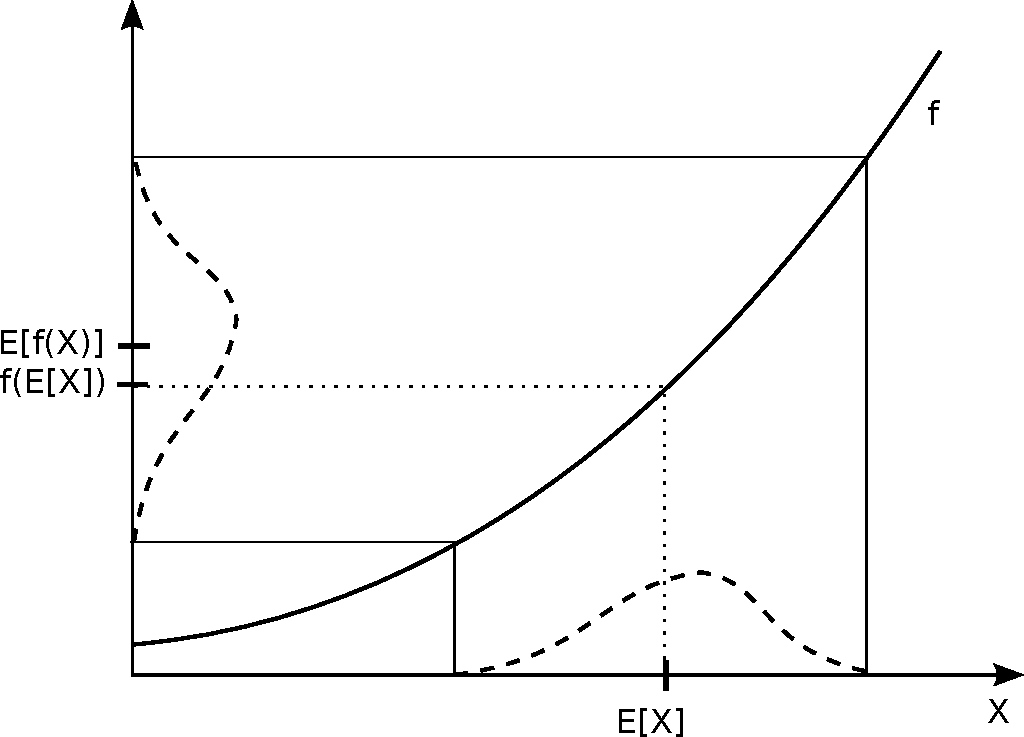
\includegraphics[width=0.5\textwidth]{images/jensen.pdf}
  %\caption{.}
  \label{fig:jensen}
  \end{figure} 

  \vspace{-0.2cm}
  O mapeamento feito pela função convexa $f$ aumenta gradativamente o estiramento
  da distribuição mapeada por $f$ com o aumento dos valores de $X$.
  Desta forma, o valor esperado da distribuição mapeada por $f$ tende a possuir
  um valor maior que o mapeamento por $f$ do valor esperado da distribuição.
\end{frame}


\subsection{Não-Negatividade}
\begin{frame}%[allowframebreaks]
  \frametitle{A divergência de KL é não-negativa}
  \begin{lemma} 
  \begin{equation}
  D(p||q) \geq 0 \text{ com igualdade se e somente se } p(x) = q(x) \forall x.
  \end{equation}
  \end{lemma}
\end{frame}

\begin{frame}%[allowframebreaks]
  \frametitle{A divergência de KL é não-negativa} 
  \begin{proof}
  Mostre que $-D(p||q) \leq 0$. Seja $S_p=\{x: p(x) > 0\} = \sup (p)$, então
  \begin{eqnarray}
  -D(p||q) &=& -\sum_x p(x) \log \frac{p(x)}{q(x)} = -\sum_{x \in S_p} p(x) \log \frac{p(x)}{q(x)} %\nonumber \\
        = \sum_{x \in S_p} p(x) \log \frac{q(x)}{p(x)} = E \log \frac{q(X)}{p(X)} \nonumber \\
        && {\small \text{utilizando a desigualdade de Jensen}} \nonumber \\
        &\leq& \log \left( E \frac{q(X)}{p(X)} \right) = \log \left( \sum_{x \in S_p} p(x) \frac{q(x)}{p(x)} \right) \nonumber \\
        &=& \log \left( \sum_{x \in S_p} q(x) \right) \leq \log \left( \sum_x  q(x) \right) = \log 1 = 0
  \end{eqnarray}
  \end{proof}
\end{frame}

\begin{frame}%[allowframebreaks]
  \frametitle{A divergência de KL é não-negativa}
  \begin{itemize}
  \item Note que $\log x$ é estritamente côncavo.
  \item Então, a igualdade $\sum_{x \in S_p} p(x) \frac{q(x)}{p(x)} = \log \left( \sum_{x \in S_p} p(x) \frac{q(x)}{p(x)} \right)$ significa $Z=E Z$ com $Z = q(X)/p(X)$, então $Z$ é uma variável aleatória constante.
  \item A única constante válida, com $p$ e $q$ sendo distribuições de probabilidade é
  $Z=1$ ou $p(x)=q(x)$.
  \item Então, se $p(x)=q(x)$ teremos $D(p||q)=0$ e vice-versa.
  \end{itemize}
\end{frame}

\begin{frame}%[allowframebreaks]
  \frametitle{A informação mútua é não-negativa}
  \begin{proposition}
  \begin{equation} 
  I(X;Y) \geq 0 \text{ e } I(X;Y) = 0 \Leftrightarrow X \independent Y.
  \end{equation}
  \end{proposition}

  \begin{proof}
  \begin{equation}
  I(X;Y) = D(p(x,y)||p(x)p(y)) \geq 0
  \end{equation}
  \end{proof}
  teremos igualdade se $p(x,y)=p(x)p(y)$, o que é também condição para independência.
\end{frame}

\begin{frame}%[allowframebreaks]
  \frametitle{Informação Mútua}
  \begin{itemize}
  \item $I(X;Y)$ mede o `grau de dependência' entre $X$ e $Y$.
  \item Temos $0 \leq I(X;Y) \leq \min (H(X),H(Y))$.
  \item $I(X;Y) = H(X) - H(X|Y) = H(Y) - H(Y|X)$.
  \item Se $X \independent Y$, então $I(X;Y)=0$, já que em tal caso $H(X|Y)=H(X)$
  e $H(Y|X)=H(Y)$.
  \item Se $X=Y$, então $I(X;Y) = H(X) = H(Y)$ já que em tal caso $H(Y|X)=H(X|Y)=0$.
  \end{itemize}
\end{frame}


\subsection{Limite Superior para a Entropia}
\begin{frame}[allowframebreaks]
  \frametitle{Limite Superior para a Entropia}
  \begin{theorem}
  $H(X) \leq \log \vert \mathcal{X} \vert$, onde $\vert \mathcal{X} \vert$ denota
  o número de elementos da extensão de $X$ (a cardinalidade do domínio), com igualdade
  se e somente se $X$ possuir distribuição uniforme.
  \end{theorem}

  \framebreak

  \begin{proof}
  Seja $u(x) = \frac{1}{\vert \mathcal{X} \vert}$ a função probabilidade de massa uniforme
  em $\mathcal{X}$, e seja $p(x)$ a função probabilidade de massa para $X$. Então
  \begin{eqnarray}
  D(p||u) &=& \sum_{x \in \mathcal{X}} p(x) \log \frac{p(x)}{u(x)} \nonumber \\
        &=& \sum_{x \in \mathcal{X}} p(x) \log p(x) + \sum_{x \in \mathcal{X}} p(x) \log \frac{1}{u(x)} \nonumber \\
        &=& -H(X) + \log \vert \mathcal{X} \vert \sum_{x \in \mathcal{X}} p(x) \nonumber \\
        &=& \log \vert \mathcal{X} \vert - H(X)
  \end{eqnarray}
  \proofbreak
  Como a entropia relativa é não negativa, $D(p||u) \geq 0$, teremos
  \begin{equation}
  D(p||u) = \log \vert \mathcal{X} \vert - H(X) \geq 0
  \end{equation}
  e assim
  \begin{equation}
  H(X) \leq \log \vert \mathcal{X} \vert
  \end{equation}
  \end{proof}
\end{frame}


\subsection{Condicionar Reduz Entropia}
\begin{frame}%[allowframebreaks]
  \frametitle{Condicionar Reduz Entropia}
  Comparando $H(X)$ com $H(X|Y)$, conhecendo $Y$, na média, pode nos dizer algo sobre $X$
  reduzindo a entropia.
  \begin{proposition}
  \begin{equation}
  H(X|Y) \leq H(X) \text{ e } H(X|Y) = H(X) \text{ se e somente se } X \independent Y.
  \end{equation}
  \end{proposition}

  \begin{proof}
  \begin{equation}
  0 \leq I(X;Y) = H(X) - H(X|Y)
  \end{equation}
  \end{proof}

  Poderíamos ter $H(X|Y=y) > H(X)$, mas, na média, $\sum_y p(y) H(X|Y=y) \leq H(X)$.
\end{frame}


\begin{frame}%[allowframebreaks]
  \frametitle{Limite da Entropia para um Conjunto de V.A.}
  A entropia de um conjunto de variáveis aleatórias é maior quando as
  variáveis aleatórias são independentes, há menor redundância entre elas.
  \begin{proposition}\label{prop-lim-ent-conj-va}
  \begin{equation}\label{eq-lim-ent-conj-va}
  H(X_1, X_2, \ldots, X_N) \leq \sum_{i=1}^N H(X_i)
  \end{equation}
  \end{proposition}

  \begin{proof}
  \begin{equation}
  H(X_1, \ldots, X_N) = \sum_{i=1}^N H(X_i | X_1, \ldots, X_{i-1}) \leq \sum_{i=1}^N H(X_i)
  \end{equation}
  \end{proof}

\end{frame}
\note{
 \begin{equation}
 \sum_{i=1}^N H(X_i | X_{\neg i}) = \sum_{i=1}^N H(X_i | X_1, \ldots, X_{i-1}, X_{i+1}, \ldots, X_N) \leq H(X_1, \ldots, X_N)
 \end{equation}
}

\begin{frame}%[allowframebreaks]
  \frametitle{Limites da Independência na Entropia}
  A proposição \ref{prop-lim-ent-conj-va} para duas variáveis é da forma
  \begin{equation}
  H(X_1,X_2) \leq H(X_1) + H(X_2)
  \end{equation}
  Note que a igualdade na Equação \ref{eq-lim-ent-conj-va} é alcançada quando
  todas as variáveis são mutuamente independentes, isto é, quando $X_i \independent X_j \forall i,j$.
\end{frame}


\begin{frame}%[allowframebreaks]
  \frametitle{Condicionamento e Informação Mútua}
  \begin{itemize}
  \item Se $X \independent Y|Z$ então $I(X;Y|Z)=0$. Por exemplo, $X \independent Y|Z$ quando
  $X \rightarrow Z \rightarrow Y$.
  \item Alternativamente, se $Z=Y$, então $I(X;Y|Z)=0$.
  \item Podemos ter $I(X;Y) > I(X;Y|Z)$.
  \item Por outro lado, se $Z=X+Y$ e $X \independent Y$, então $I(X;Y)=0$ mas 
  $I(X;Y|Z)>0$.
  \item Não existe uma relação genérica entre informação mútua e informação mútua condicional.
  \end{itemize}
\end{frame}

\begin{frame}%[allowframebreaks]
  \frametitle{Relações de H}

  \begin{equation}
  H(X) = E I(X) = - \sum_x p(x) \log p(x)
  \end{equation}

  \begin{equation}
  H(X,Y) = - \sum_{x,y} p(x,y) \log p(x,y)
  \end{equation}

  \begin{equation}
  H(Y|X) = - \sum_{x,y} p(x,y) \log p(y|x)
  \end{equation}

  \begin{equation}
  H(X,Y) = H(X) + H(Y|X) = H(Y) + H(X|Y)
  \end{equation}

  \begin{equation}
  I(X;Y) = H(X) - H(X|Y) = H(Y) - H(Y|X)
  \end{equation}

  \begin{equation}
  0 \leq H(X) \leq \log n, \text{ onde } n \text{ é o tamanho do alfabeto de } X.
  \end{equation}
\end{frame}

\begin{frame}%[allowframebreaks]
  \frametitle{Entropia, Informação Mútua, 3 V.A. em um diagrama de Venn}
  \begin{figure}[h!]
  \centering
  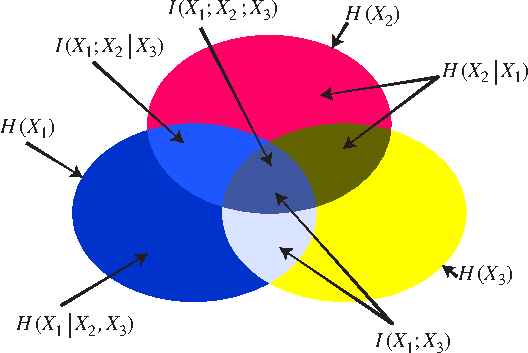
\includegraphics[width=0.7\textwidth]{images/3va-venn.pdf}
  %\caption{.}
  \label{fig:3va-venn}
  \end{figure}
\end{frame}
\note{
\begin{itemize}
 \item $I(X_1;X_2) = I(X_1;X_2|X_3) + I(X_1;X_2;X_3)$.
 \item $I(X_1;X_2) \gtreqqless I(X_1;X_2|X_3)$, mas isto nunca será negativo. 
 \item Então, $I(X_1;X_2;X_3) = I(X_1;X_2) - I(X_1;X_2|X_3)$ pode ser negativo.
 \item $I(X_1;X_2;X_3) = I(X_1;X_2) - I(X_1;X_2|X_3) = I(X_2;X_3) - I(X_2;X_2|X_1) = I(X_3;X_1) - I(X_3;X_1|X_2)$
 \item $I(X_1;X_2;X_3) = H(X_1) + H(X_2) + H(X_3) - H(X_1;X_2) - H(X_2;X_3) - H(X_3;X_1) + H(X_1,X_2,X_3)$
\end{itemize}
}


\begin{frame}[allowframebreaks]
  \frametitle{Revisão}
  \begin{itemize}
  \item divergência de KL: $D(p||q) = \sum_x p(x) \log \frac{p(x)}{q(x)}$
  \item informação mútua: $I(X;Y) = \sum_{x,y} p(x,y) \log \frac{p(x,y)}{p(x)p(y)} = D(p(x,y)||p(x)p(y))$ 
  \item informação mútua condicional: $I(X;Y|Z) = \sum_{x,y,z} p(x,y,z) \log \frac{p(x,y|z)}{p(x|z) p(y|z)} = H(X|Z) - H(X|Y,Z)$
  \item regra da cadeia da informação mútua: $I(X_1,X_2,\ldots,X_N;Y)=\sum_i I(X_i;Y|X_1,X_2,\ldots,X_{i-1})$
  \item entropia relativa condicional: $D(p(y|x)||q(y|x)) \triangleq \sum_{x,y} p(x,y) \log \frac{p(y|x)}{q(y|x)}$
  \item regra da cadeia da divergência de KL: $D(p(x,y)||q(x,y)) = D(p(x)||q(x)) + D(p(y|x)||q(y|x))$
  \item Jensen: $f$ convexa $\Rightarrow$ $E f(X) = \sum_x p(x) f(x) \geq f(E X) = f \left( \sum_x p x(x) \right)$
  \item não negatividade da divergência de KL: $D(p||q) \geq 0$, $D(p||q)=0 \Leftrightarrow p=q$.
  \item não negatividade da informação mútua: $I(X;Y)\geq 0$, $I(X;Y)=0 \Leftrightarrow X \independent Y$.
  \item condicionar reduz a entropia: $H(X) \geq H(X|Y)$, $H(X) = H(X|Y) \Leftrightarrow X \independent Y$.
  \item limite da independência em H: $H(X_1,\ldots,X_N) \leq \sum_{i} H(X_i)$, com igualdade sse todos $X_i$ forem independentes
  \end{itemize}
\end{frame}



\subsection{Medida de Informação}
\begin{frame}%[allowframebreaks]
  \frametitle{Medida de Informação}
  Veremos as correspondências entre a medida de informação de Shannon (e suas manipulações)
  com a teoria de conjuntos. A utilização dos diagramas de informação podem ser utilizadas para 
  simplificar várias demonstrações em teoria da informação.
\end{frame}

\begin{frame}%[allowframebreaks]
  \frametitle{Medida de Informação}
  \begin{itemize}
  \item Temos um conjunto de variáveis aleatórias: $X_1, X_2, \ldots, X_n$.
  \item Para cada variável aleatória associamos um conjunto $\tilde{X}_1, \tilde{X}_2, \ldots, \tilde{X}_n$.
  \end{itemize}

  \begin{definition}[campo (field)]
  Um campo $\mathcal{F}_n$ gerado pelos conjuntos $\tilde{X}_1, \tilde{X}_2, \ldots, \tilde{X}_n$ é
  a coleção de conjuntos que podem ser obtidos através de qualquer sequência de operações
  usuais de conjuntos (união, interseção, complemento, e diferença) sobre os conjuntos 
  $\tilde{X}_1, \tilde{X}_2, \ldots, \tilde{X}_n$.
  \end{definition}

  \begin{definition}[átomo]
  Os átomos de $\mathcal{F}_n$ são os conjuntos da forma $\cap_{i=1}^n Y_i$, onde 
  $Y_i$ é $\tilde{X}_i$ ou $\tilde{X}_i^c$, o complemento de $\tilde{X}_i$.
  \end{definition}
\end{frame}

\begin{frame}%[allowframebreaks]
  \frametitle{Átomos}
  \begin{exampleblock}{átomos - $n=2$}
  Para $n=2$, teremos os conjuntos $\tilde{X}_1, \tilde{X}_2$ e seus complementos,
  respectivamente, $\tilde{X}_1^c, \tilde{X}_2^c$. Existirão $4$ átomos:

  \begin{minipage}[t]{0.35\linewidth}
  \begin{enumerate}
  \item $\tilde{X}_1 \cap \tilde{X}_2$,
  \item $\tilde{X}_1 \cap \tilde{X}_2^c$,
  \item $\tilde{X}_1^c \cap \tilde{X}_2$, e
  \item $\tilde{X}_1^c \cap \tilde{X}_2^c$
  \end{enumerate}
  \end{minipage} \hfill 
  \begin{minipage}[t]{0.55\linewidth}
    \begin{figure}[!ht]
    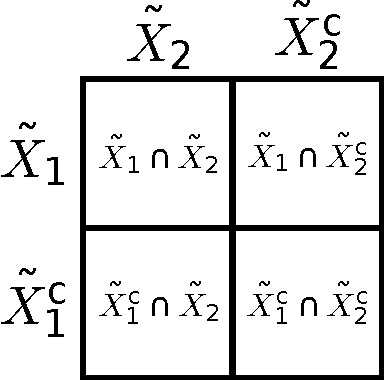
\includegraphics[width=0.5\linewidth]{images/atoms-n2.pdf}
    \end{figure}
  \end{minipage}

  \end{exampleblock}
\end{frame}

\begin{frame}%[allowframebreaks]
  \frametitle{Átomos}
  \begin{exampleblock}{átomos - $n=3$}
  Para $n=3$, teremos os conjuntos $\tilde{X}_1, \tilde{X}_2, \tilde{X}_3$ e seus complementos,  
  respectivamente, $\tilde{X}_1^c, \tilde{X}_2^c, \tilde{X}_3^c$. Existirão $8$ átomos:

  \begin{minipage}[t]{0.35\linewidth}
  \begin{enumerate}
  \item $\tilde{X}_1 \cap \tilde{X}_2 \cap \tilde{X}_3$,
  \item $\tilde{X}_1 \cap \tilde{X}_2 \cap \tilde{X}_3^c$,
  \item $\tilde{X}_1 \cap \tilde{X}_2^c \cap \tilde{X}_3$,
  \item $\tilde{X}_1 \cap \tilde{X}_2^c \cap \tilde{X}_3^c$,
  \item $\tilde{X}_1^c \cap \tilde{X}_2 \cap \tilde{X}_3$, 
  \item $\tilde{X}_1^c \cap \tilde{X}_2 \cap \tilde{X}_3^c$,
  \item $\tilde{X}_1^c \cap \tilde{X}_2^c \cap \tilde{X}_3$, e 
  \item $\tilde{X}_1^c \cap \tilde{X}_2^c \cap \tilde{X}_3^c$
  \end{enumerate}
  \end{minipage} \hfill
  \begin{minipage}[t]{0.6\linewidth}
    \begin{figure}[!ht]
    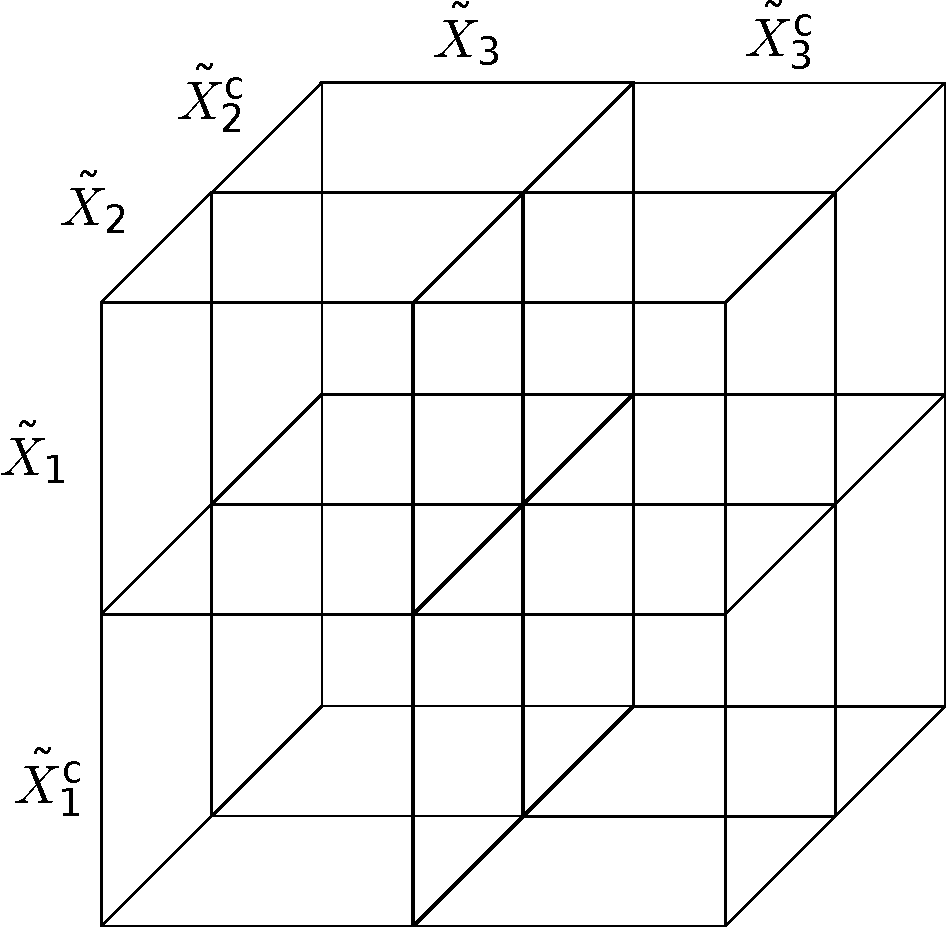
\includegraphics[width=0.6\linewidth]{images/atoms-n3.pdf}
    \end{figure}
  \end{minipage}

  \end{exampleblock}
\end{frame}

\begin{frame}%[allowframebreaks]
  \frametitle{Campo e Átomos}
  \begin{itemize}
  \item existem $2^n$ átomos;
  \item existem $2^{2^n}$ conjuntos no campo $\mathcal{F}_n$;
  \item todos os átomos em $\mathcal{F}_n$ são disjuntos;
  \item todo conjunto em $\mathcal{F}_n$ pode ser expresso de forma única como uma união de um subconjunto dos átomos em $\mathcal{F}_n$.
  \end{itemize}
\end{frame}

\begin{frame}%[allowframebreaks]
  \frametitle{Medida com sinal}
  Em análise matemática, uma medida em um conjunto $S$ é uma forma sistemática de atribuir
  números a todo subconjunto de $S$, sendo intuitivamente interpretada como o seu tamanho.

  Medida com sinal é uma generalização do conceito de medida permitindo que esta assuma valores
  negativos.

  \begin{definition}[medida com sinal]
  Uma função real $\mu$ definida em $\mathcal{F}_n$ é chamada medida com sinal se
  for aditiva no conjunto, i.e., para $A$ e $B$ disjuntos em $\mathcal{F}_n$,
  \begin{equation}
  \mu(A \cup B) = \mu(A) + \mu(B) .
  \end{equation} 
  \end{definition}  
  Para uma medida com sinal $\mu$ teremos $\mu(\emptyset)=0$, já que
  $\mu(A) = \mu(A \cup \emptyset) = \mu(A) + \mu(\emptyset)$.
\end{frame}

\begin{frame}%[allowframebreaks]
  \frametitle{Medida com sinal}
  Uma medida com sinal $\mu$ em $\mathcal{F}_n$ é completamente especificada
  por seus valores nos átomos de $\mathcal{F}_n$. Os valores de $\mu$ em outros
  conjuntos de $\mathcal{F}_n$ podem ser obtidos pela aditividade de conjuntos, 
  já que qualquer $\tilde{X} \in \mathcal{F}_n$ pode ser representado como
  $\tilde{X} = \cup_{i=1} Y_i$, onde $Y_i$ são átomos escolhidos apropriadamente.
\end{frame}


\begin{frame}%[allowframebreaks]
  \frametitle{Medida com sinal}
  \begin{exampleblock}{$n=2$}
  Uma medida com sinal $\mu$ em $\mathcal{F}_2$ é completamente especificada pelos
  valores 
  $\mu( \tilde{X}_1 \cap \tilde{X}_2 )$,
  $\mu( \tilde{X}_1 \cap \tilde{X}_2^c )$,
  $\mu( \tilde{X}_1^c \cap \tilde{X}_2 )$, e
  $\mu( \tilde{X}_1^c \cap \tilde{X}_2^c )$.

  O valor de $\mu$ em $\tilde{X}_1$ pode ser obtido da seguinte forma
  \begin{eqnarray}
  \mu( \tilde{X}_1 ) &=& \mu( (\tilde{X}_1 \cap \tilde{X}_2) \cup ( \tilde{X}_1 \cap \tilde{X}_2^c) ) \nonumber \\
		&=& \mu( \tilde{X}_1 \cap \tilde{X}_2 ) + \mu( \tilde{X}_1 \cap \tilde{X}_2^c ) .
  \end{eqnarray}

  O valor de $\mu$ em $\tilde{X}_1 \setminus \tilde{X}_2$ é dado por
  \begin{equation}
  \mu( \tilde{X}_1 \setminus \tilde{X}_2 ) = \mu( \tilde{X}_1 \cap \tilde{X}_2^c ) .
  \end{equation}

  O valor de $\mu$ em $\tilde{X}_1 \cup \tilde{X}_2$ pode ser obtido através de
  \begin{eqnarray}
  \mu( \tilde{X}_1 \cup \tilde{X}_2 ) &=& \mu( (\tilde{X}_1 \cap \tilde{X}_2) \cup (\tilde{X}_1 \cap \tilde{X}_2^c) \cup (\tilde{X}_1^c \cap \tilde{X}_2) ) \nonumber \\
	&=& \mu( \tilde{X}_1 \cap \tilde{X}_2 ) + \mu( \tilde{X}_1 \cap \tilde{X}_2^c ) + \mu(\tilde{X}_1^c \cap \tilde{X}_2) 
  \end{eqnarray}

  \end{exampleblock}
\end{frame}


\begin{frame}[allowframebreaks]
  \frametitle{Correspondência com a informação de Shannon}
  Os conjuntos $\tilde{X}_1$ e $\tilde{X}_2$ estão associados às variáveis
  aleatória $X_1$ e $X_2$. O campo $\mathcal{F}_2$ é gerado por $\tilde{X}_1$ e $\tilde{X}_2$,
  através dos átomos 
  $(\tilde{X}_1 \cap \tilde{X}_2)$,
  $(\tilde{X}_1 \cap \tilde{X}_2^c)$,
  $(\tilde{X}_1^c \cap \tilde{X}_2)$, e
  $(\tilde{X}_1^c \cap \tilde{X}_2^c)$.
  O diagrama de informação é apresentado na Figura \ref{fig:setX1X2}.

  \begin{figure}[h!]
  \centering
  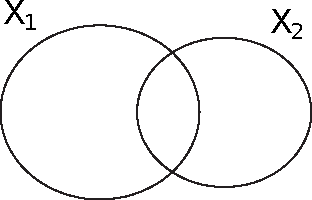
\includegraphics[width=0.4\textwidth]{images/setX1X2.pdf}
  \caption{Diagrama de informação para $X_1$ e $X_2$.}
  \label{fig:setX1X2}
  \end{figure}
 
  O conjunto universo será considerada como sendo $\Omega = \tilde{X}_1 \cup \tilde{X}_2$.
  Desta forma, o átomo $\tilde{X}_1^c \cap \tilde{X}_2^c$ se degenera ao conjunto vazio,
  \begin{equation}
  \tilde{X}_1^c \cap \tilde{X}_2^c = (\tilde{X}_1 \cup \tilde{X}_2)^c = \Omega^c = \emptyset .
  \end{equation}

  Para as v.a.s $X_1$ e $X_2$, as medidas de informação de Shannon são 
  \begin{equation}
  H(X_1), H(X_2), H(X_1|X_2), H(X_2|X_1), H(X_1,X_2), I(X_1;X_2) .
  \end{equation}

  Utilizando a notação $A \cap B^c \equiv A \setminus B$, definimos uma medida com sinal $\mu^\ast$
  \begin{eqnarray}
  \mu^\ast(\tilde{X}_1 \setminus \tilde{X}_2) &=& H(X_1|X_2) ,\\
  \mu^\ast(\tilde{X}_2 \setminus \tilde{X}_1) &=& H(X_2|X_1) ,\\
  \mu^\ast(\tilde{X}_1 \cap \tilde{X}_2) &=& I(X_1;X_2) .
  \end{eqnarray}
  Estes são os valores de $\mu^\ast$ nos átomos não vazios de $\mathcal{F}_2$.
  Os valores de $\mu^\ast$ nos demais conjuntos de $\mathcal{F}_2$ podem ser obtidos por
  adição de conjuntos. Em particular, temos as relações
  \begin{eqnarray}
  \mu^\ast(\tilde{X}_1 \cup \tilde{X}_2) &=& H(X_1, X_2) , \label{eqX1X2HX1X2} \\
  \mu^\ast(\tilde{X}_1) &=& H(X_1) , \label{eqmuX1HX1}\\
  \mu^\ast(\tilde{X}_2) &=& H(X_2) .
  \end{eqnarray}

  Por exemplo, a Equação \ref{eqX1X2HX1X2} pode ser verificada
  \begin{eqnarray}
  \mu^\ast(\tilde{X}_1 \cup \tilde{X}_2) &=& \mu^\ast( (\tilde{X}_1 \setminus \tilde{X}_2) \cup (\tilde{X}_2 \setminus \tilde{X}_1) \cup (\tilde{X}_1 \cap \tilde{X}_2) ) \nonumber \\
	&=& \mu^\ast( \tilde{X}_1 \setminus \tilde{X}_2 ) + \mu^\ast( \tilde{X}_2 \setminus \tilde{X}_1 ) + \mu^\ast( \tilde{X}_1 \cap \tilde{X}_2 ) \nonumber \\
	&=& H(X_1|X_2) + H(X_2|X_1) + I(X_1;X_2) \nonumber \\
	&=& H(X_1, X_2) .
  \end{eqnarray}

  A Equação \ref{eqmuX1HX1} também pode ser facilmente verificada
  \begin{eqnarray}
  \mu^\ast(\tilde{X}_1) &=& \mu^\ast( (\tilde{X}_1 \cap \tilde{X}_2) \cup (\tilde{X}_1 \cap \tilde{X}_2^c) ) \nonumber \\
	&=& \mu^\ast(\tilde{X}_1 \cap \tilde{X}_2) + \mu^\ast(\tilde{X}_1 \cap \tilde{X}_2^c) \nonumber \\
	&=& I(X_1;X_2) + H(X_1|X_2) = H(X_1) .
  \end{eqnarray}

  É possível então verificar a seguinte correspondência com as medidas de informação de Shannon
  \begin{eqnarray}
  H / I &\leftrightarrow& \mu^\ast \\
  , &\leftrightarrow& \cup \\
  ; &\leftrightarrow& \cap \\
  | &\leftrightarrow& \setminus 
  \end{eqnarray}

  \begin{itemize}
  \item obs.: com a notação de medida, não existe distinção entre $H$ e $I$, podemos escrever
	$H(X;Y) = I(X;Y)$, utilizando a notação do ponto-e-vírgula.
  \end{itemize}
\end{frame}



\subsection{Desigualdade da soma de logaritmos}
\begin{frame}%[allowframebreaks]
  \frametitle{Desigualdade da soma de logaritmos}
  \begin{theorem}[desigualdade da soma de logaritmos]
  Dados $(a_1, \ldots, a_n)$ e $(b_1,\ldots,b_n)$, com $a_i \geq 0$ e $b_i \geq 0$, temos
        \begin{equation}
         \sum_{i=1}^n a_i \log \frac{a_i}{b_i} \geq \left( \sum_{i=1}^n a_i \right) \log \frac{\sum_{i=1}^n a_i}{\sum_{i=1}^n b_i}
        \end{equation}
  e teremos igualdade sse $a_i/b_i = c = \text{const.}$.
  \end{theorem}

  \begin{itemize}
  \item Relembrando: $0 \log 0 = 0$, $a \log a/0 = \infty$ para $a>0$, e $0 \log 0/0 =0$.
  \item A desigualdade da soma de logaritmos é utilizada para demonstrar algumas propriedades importantes.
  \end{itemize}
\end{frame}

\begin{frame}%[allowframebreaks]
  \frametitle{Desigualdade da soma de logaritmos}

  Considere $f(t) = t \log t = t (\ln t) (\log e)$, que é estritamente convexa, pois
  $f''(t) = 1/t \log e >0$, $\forall t > 0$.
  
  \begin{figure}[h!]
  \centering
  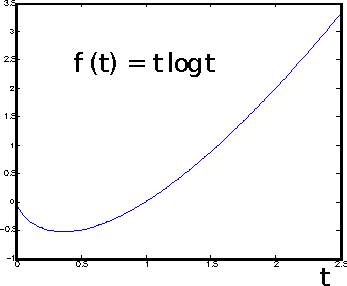
\includegraphics[width=0.4\textwidth]{images/tlogt.pdf}
  %\caption{.}
  \label{fig:tlogt}
  \end{figure}
\end{frame}

\begin{frame}[allowframebreaks]
  \frametitle{Desigualdade da soma de logaritmos}
  \begin{proof}
        \begin{itemize}
        \item Dada $f$ convexa, a desigualdade de Jensen diz que
          \begin{equation}
          \sum_i \alpha_i f(t_i) \geq f \left( \sum_i \alpha_i t_i \right) \text{ com } \alpha_i \geq 0 \text{ e } \sum_i \alpha_i = 1
          \end{equation}

        \item $f(x) = x \log x$ é estritamente convexa para $x>0$, já que 
                $f''(x)=\frac{1}{x} \log e > 0$ para $x>0$.

        \end{itemize}
        \proofbreak
        \begin{itemize}
        \item Vamos fazer $\alpha_i = \nicefrac{b_i}{\sum_{j=1}^n b_j}$ e $t_i = \nicefrac{a_i}{b_i}$, então teremos
        \begin{eqnarray}
        \sum_i \alpha_i f(t_i) &\geq& f \left( \sum_i \alpha_i t_i \right) \nonumber \\
        \sum_i \left( \frac{b_i}{\sum_j b_j} f \left( \frac{a_i}{b_i} \right) \right) &\geq&
                f \left( \sum_i \frac{b_i}{\sum_j b_j} \frac{a_i}{b_i} \right) \nonumber
        \end{eqnarray}
        \end{itemize}

   \proofbreak
   \vspace{-2ex}
   \begin{eqnarray}
        \sum_i \left( \frac{b_i}{\sum_j b_j} f \left( \frac{a_i}{b_i} \right) \right) &\geq&
                f \left( \sum_i \frac{b_i}{\sum_j b_j} \frac{a_i}{b_i} \right) \nonumber \\
        \frac{1}{\sum_j b_j} \sum_i \left( b_i \frac{a_i}{b_i} \log \frac{a_i}{b_i} \right) &\geq&
                \left( \sum_i \frac{a_i}{\sum_j b_j} \right) \log \sum_i \frac{a_i}{\sum_j b_j} \nonumber \\
        \sum_i a_i \log \frac{a_i}{b_i} &\geq& \left( \sum_i a_i \right) \log \sum_i \frac{a_i}{\sum_j b_j} \nonumber \\
        \sum_i a_i \log \frac{a_i}{b_i} &\geq& \sum_i a_i \log \frac{\sum_i a_i}{\sum_j b_j}
   \end{eqnarray}

  \end{proof}
\end{frame}


\subsection{Divergência é não negativa}
\begin{frame}%[allowframebreaks]
  \frametitle{Divergência é não negativa}
  A desigualdade da soma de logaritmos pode ser utilizada para mostrar que $D(p||q) \geq 0$.
  \begin{proof}
        \begin{eqnarray}
        D(p||q) &=& \sum_x p(x) \log \frac{p(x)}{q(x)} \nonumber \\
                &\geq& \left( \sum_x p(x) \right) \log \frac{\sum_x p(x)}{\sum_x q(x)} \nonumber \\
                &=& 1 \log \frac{1}{1} = 0
        \end{eqnarray}
  \end{proof}
\end{frame}

\subsection{Entropia Relativa é Convexa no Par}
\begin{frame}[allowframebreaks]
  \frametitle{A Entropia Relativa é Convexa no Par}
  \begin{theorem}
  Seja $(p_1, q_1)$ e $(p_2, q_2)$ dois pares de função massa probabilidade, então
    \begin{equation}
        D(\lambda p_1 + (1 - \lambda) p_2 || \lambda q_1 + (1- \lambda)q_2) \leq \lambda D(p_1 || q_1) + (1- \lambda) D(p_2 || q_2) ,
    \end{equation}
    para todo $0 \leq \lambda \leq 1$.
  \end{theorem}

  \framebreak

  \begin{proof}
  Pela definição da divergência de KL, temos
    \begin{multline}
    D(\lambda p_1 + (1 - \lambda) p_2 || \lambda q_1 + (1- \lambda)q_2) = \\
        \sum_x (\lambda p_1(x) + (1 - \lambda) p_2(x) ) \log \frac{\lambda p_1(x) + (1 - \lambda) p_2(x)}{\lambda q_1(x) + (1 - \lambda) q_2(x)}
    \end{multline}
    cada termo do somatório é da forma
    \begin{equation}
        ( \lambda p_1(x) + (1 - \lambda) p_2(x) ) \log \frac{\lambda p_1(x) + (1 - \lambda) p_2(x)}{\lambda q_1(x) + (1 - \lambda) q_2(x)} = \left( \sum_i a_i \right) \log \frac{\sum_i a_i}{\sum_i b_i}
    \end{equation}

  \proofbreak

  Utilizando a desigualdade da soma dos logaritmos 
  \begin{eqnarray}
  \left( \sum_i a_i \right) \log \frac{\sum_i a_i}{\sum_i b_i} &\leq&
        \sum_i a_i \log \frac{a_i}{b_i} \nonumber \\
        &=& a_1 \log \frac{a_1}{b_1} + a_2 \log \frac{a_2}{b_2} \nonumber \\
        &=& \lambda p_1(x) \log \frac{\lambda p_1(x)}{\lambda q_1(x)} + (1 - \lambda) p_2(x) \log \frac{(1 - \lambda) p_2(x)}{(1-\lambda) q_2(x)} \nonumber \\
        &=& \lambda D(p_1 || q_1) + (1 - \lambda) D(p_2 || q_2)
  \end{eqnarray}
  \end{proof}
\end{frame}
\note{
        \begin{itemize}
        \item Note que podemos fazer $q_1 = q_2$ e desta forma obteremos convexidade apenas em $p$.
        \item Este é o fundamento para o procedimento de minimização alternada, que
        é um caso especial do algoritmo de EM (maximização da esperança), 
        para o cálculo da função de taxa de distorção,
        e para o cálculo da função geral de capacidade de canal.
        \end{itemize}
}

\subsection{Concavidade da Entropia}
\begin{frame}[allowframebreaks]
  \frametitle{A Entropia é Concava}
  \begin{theorem}
  $H(p)$ é uma função concava de $p$.
  \end{theorem}

  \framebreak
  \begin{proof}
  \vspace{-4ex}
  \begin{eqnarray}
    H(p) &=& - \sum_i p_i \log p_i = - \sum_i p_i \log p_i  + \log \vert \mathcal{X} \vert - \log \vert \mathcal{X} \vert \nonumber \\
        &=& \log \vert \mathcal{X} \vert - \sum_i p_i \log p_i - \log \vert \mathcal{X} \vert \underbrace{\sum_i p_i}_{=1} \nonumber \\
        &=& \log \vert \mathcal{X} \vert - \sum_i \left( p_i \log p_i + p_i \log \vert \mathcal{X} \vert \right) \nonumber \\
        &=& \log \vert \mathcal{X} \vert - \sum_i p_i \left( \log p_i -  \log \nicefrac{1}{\vert \mathcal{X} \vert } \right) \nonumber \\
        &=& \underbrace{\log \vert \mathcal{X} \vert}_{\text{constante}} - \underbrace{D(p||u)}_{\text{convexo}}
  \end{eqnarray}
  onde $u$ é a distribuição uniforme.
  \end{proof}
\end{frame}
\note{
Podemos ver a entropia como a similaridade com a distribuição uniforme.
Quanto maior a entropia, mais próximo estaremos da distribuição uniforme.
}

\begin{frame}[allowframebreaks]
  \frametitle{Consequências para a Informação Mútua}
  Seja $(X,Y) \sim p(x,y) = p(x)p(y|x)$, a informação mútua $I(X;Y)$ é uma função côncava
  de $p(x)$ para $p(y|x)$ fixo e uma função convexa de $p(y|x)$ para $p(x)$ fixo.

  \framebreak
  \begin{proof}
    \begin{itemize} \item $I(X;Y)$ é uma função côncava de $p(x)$ para $p(y|x)$ fixo \end{itemize}
    \vspace{-2ex}
    \begin{eqnarray}
    I(X;Y) &=& D(p(x,y)||p(x)p(y)) \text{ (definição) } \nonumber \\
        &=& \sum_{x,y} p(x,y) \log \frac{p(x,y)}{p(x)p(y)} \text{ (definição) } \nonumber \\
        &=& \sum_{x,y} p(x)p(y|x) \log \frac{ p(x)p(y|x) }{p(x) \sum_x p(x) p(y|x)}
    \end{eqnarray}
    Se $p(y|x)$ é constante, então a informação mútua é função de $p(x)$
    \vspace{-1ex}
    \begin{equation}
    I_{p(x)} (X;Y) = \sum_{x,y} p(x) p(y|x) \log \frac{p(x) p(y|x)}{p(x) \sum_x p(x) p(y|x)}
    \end{equation}  

    \proofbreak
    
    \begin{equation}
    I_{p(x)} (X;Y) = \sum_{x,y} p(x) p(y|x) \log \frac{p(x) p(y|x)}{p(x) \sum_x p(x) p(y|x)}
    \end{equation}

    Utilizando a propriedade da convexidade da divergência de Kullback-Leibler
    \begin{equation}\label{eq-Imixpx}
    I_{\lambda p_1(x) + (1-\lambda)p_2(x)} (X;Y) \geq \lambda I_{p_1(x)} (X;Y) + (1-\lambda) I_{p_2(x)} (X;Y)
    \end{equation}
    então a informação mútua é uma função concava de $p(x)$ para $p(y|x)$ fixo.


    \proofbreak

    \begin{itemize} \item $I(X;Y)$ é uma função convexa de $p(y|x)$ para $p(x)$ fixo \end{itemize}
    Aplicamos a mesma ideia, porém agora consideraremos $p(x)$ fixo.
    \begin{equation}
    I_{p(y|x)} (X;Y) = \sum_{x,y} p(x) p(y|x) \log \frac{p(x) p(y|x)}{p(x) \sum_x p(x) p(y|x)}
    \end{equation}

    Utilizando a propriedade da convexidade da divergência de Kullback-Leibler
    \begin{equation}\label{eq-Imixpxy}
    I_{\lambda p_1(y|x) + (1-\lambda)p_2(y|x)} (X;Y) \leq \lambda I_{p_1(y|x)} (X;Y) + (1-\lambda) I_{p_2(y|x)} (X;Y)
    \end{equation}

  \end{proof}
\end{frame}
\note{
Estes resultados serão importantes para a capacidade de canal e vários outras
otimizações envolvendo informação mútua e distribuições.
}

\begin{frame}[allowframebreaks]
  \frametitle{Informação Mútua, Comunicação e Convexidade}

  Envio de informação por um canal ruidoso.
  \begin{figure}[h!]
  \centering
  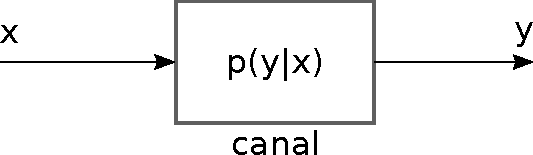
\includegraphics[width=0.5\textwidth]{images/canal_pyx.pdf}
  %\caption{.}
  \label{fig:3va-venn}
  \end{figure}

  \begin{itemize}
        \item Canal: processo ruidoso, para cada $x$ temos uma distribuição sobre os possíveis $y$ recebidos
        \item A taxa de informação transmitida de $X$ para $Y$, por utilização do canal,
        em unidades de bits, é $I(X;Y)$.
  \end{itemize}
\end{frame}
\note{
  \begin{itemize}
        \item Embaralhando $p(x)$ não pode diminuir (pode aumentar ou não alterar) 
        a transmissão de informação para um canal fixo, com relação à original mistura de taxas
        (ver Equação \ref{eq-Imixpx}).
        \item Embaralhando $p(y|x)$ para um canal ruidoso e uma fonte fixa, podemos apenas
        não aumentar (pode reduzir ou manter constante) a taxa de transmissão, em relação
        à original mistura de taxas (ver Equação \ref{eq-Imixpxy}).
  \end{itemize}
}



\section{Processamento de Dados}
\subsection{Desigualdade do Processamento de Dados}

\begin{frame}%[allowframebreaks]
  \frametitle{Desigualdade do Processamento de Dados}
  Dada uma fonte de informação, é possível utilizar alguma forma de processamento de dados
  de forma a obter mais informação sobre esta fonte?

  \begin{figure}[h!]
  \centering
  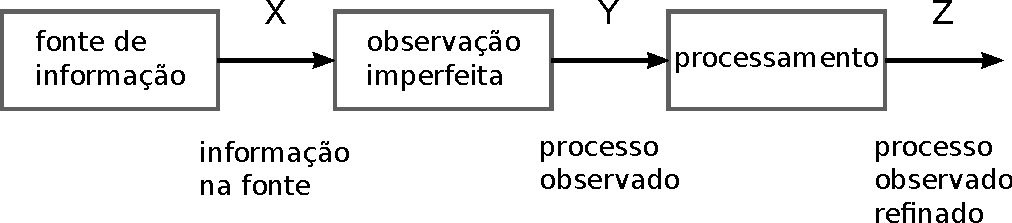
\includegraphics[width=0.8\textwidth]{images/proc-data.pdf}
  %\caption{.}
  \label{fig:proc-data}
  \end{figure} 
\end{frame}

\begin{frame}%[allowframebreaks]
  \frametitle{Desigualdade do Processamento de Dados}
  \begin{itemize}
  \item Imagens com ISO elevado são ruidosas, mas são a única forma de obtermos uma foto
        em baixa luminosidade com pequena abertura (ampla profundidade de campo).
  \item O objetivo da remoção de ruído é recuperar a imagem original.
  \end{itemize}

  \begin{figure}[h!]
  \centering
  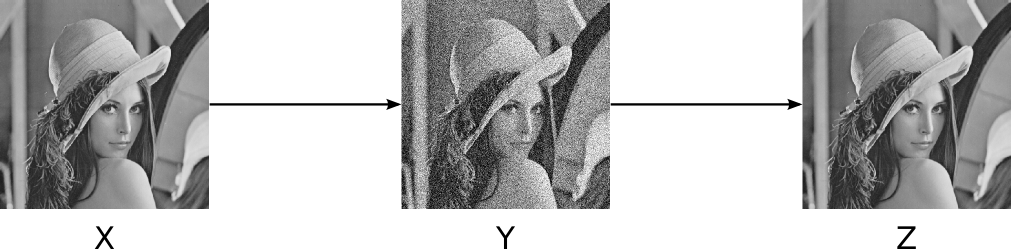
\includegraphics[width=0.8\textwidth]{images/lena-denoising.png}
  %\caption{.}
  \label{fig:lena-denoising}
  \end{figure}

  \begin{itemize}
  \item É possível obter mais informação sobre uma fonte através de processamento adicional?
  \pause
  Infelizmente não.
  \end{itemize}
\end{frame}
\note{
Profundidade de campo descreve até que ponto objetos que estão mais ou menos perto do plano de foco aparentam estar nítidos. 

Regra geral, quanto menor for a abertura do diafragma/íris (maior o valor f/x), para uma mesma distância do objecto fotografado, maior será a distância do plano de foco a que os objetos podem estar enquanto permanecem nítidos.
}

\subsection{Cadeia de Markov}
\begin{frame}[allowframebreaks]
  \frametitle{Cadeia de Markov}
  \begin{definition}[Cadeia de Markov]
  As variáveis aleatórias $X$, $Y$ e $Z$ formam uma cadeia de Markov nesta ordem
  (denotado $X \rightarrow Y \rightarrow Z$) se a distribuição condicional de $Z$
  depende apenas de $Y$ e é condicionalmente independente de $X$. Especificamente,
  $X$, $Y$ e $Z$ formam uma cadeia de Markov $X \rightarrow Y \rightarrow Z$ se
  a função massa de probabilidade conjunta pode ser escrita como
  \begin{equation}
  p(x,y,z) = p(x) p(y|x) p(z|y)
  \end{equation}
  \end{definition}

  \begin{itemize}
  \item $X \rightarrow Y \rightarrow Z$ sse $X$ e $Z$ são condicionalmente independentes
  dado $Y$ ($X \independent Z | Y$). Isto é,
  \begin{equation}
  p(x,z|y) = \frac{p(x,y,z)}{p(y)} = \frac{p(x)p(y|x)p(z|y)}{p(y)} = p(x|y) p(z|y) \ \ \forall x,y,z
  \end{equation}
  \end{itemize}

  \framebreak

  \begin{itemize}
  \item $X \rightarrow Y \rightarrow Z$ implica em $Z \rightarrow Y \rightarrow X$
  \end{itemize}
  \begin{proof}
  \begin{eqnarray}
        p(x,y,z) &=& p(x)p(y|x)p(z|y) = p(x,y)p(z|y) \nonumber \\
                &=& \frac{p(x,y)p(z|y)p(y)}{p(y)} = p(x|y) p(y,z) \nonumber \\
                &=& p(x|y) p(y|z) p(z)
  \end{eqnarray}
  \end{proof}

  \begin{figure}[h!]
  \centering
  
\includegraphics[width=0.8\textwidth]{images/chainxyz.pdf}
  %\caption{.}
  \label{fig:chain}
  \end{figure}

  \begin{itemize}
  \item Se $Z=f(Y)$, então $X \rightarrow Y \rightarrow Z$ (i.e., $X$, $Y$ e $Z$ formam
        uma cadeia de Markov). $f(\cdot)$ pode ser aleatória ou determinística. 
        $X$ é irrelevante para determinar $Z$ quando $Y$ é dado.
  \end{itemize}
\end{frame}

\begin{frame}[allowframebreaks]
  \frametitle{Desigualdade do Processamento de Dados}
  \begin{theorem}[Desigualdade do Processamento de Dados]
   Se $X \rightarrow Y \rightarrow Z$ então
  \begin{equation}
        I(X;Y) \geq I(X;Z)
  \end{equation}
  \end{theorem}
  \begin{itemize}
  \item Na cadeia de Markov, as setas correspondem ao processamento e as variáveis aleatórias 
        correspondem aos dados.
  \item O processamento pode ser aleatório ou determinístico.
  \item A desigualdade de processamento de dados diz que ao efetuar mais processamento dos dados,
        só é possível perder informação sobre a fonte original, quando medida pela informação mútua.
  \end{itemize}

  \framebreak

  \begin{proof}
  Utilizando a regra da cadeia da informação mútua, teremos
  \begin{eqnarray}
  I(X;Y,Z) &=& I(X;Z) + I(X;Y|Z) \nonumber \\
        &=& I(X;Y) + I(X;Z|Y)
  \end{eqnarray}
  Como $X \independent Z |Y$ ($X$ e $Z$ são condicionalmente independentes, dado $Y$), temos
  que $I(X;Z|Y)=0$. Como $I(X;Y|Z) \geq 0$, teremos
  \begin{equation}
  I(X;Z) + \underbrace{I(X; Y|Z)}_{\geq 0} = I(X;Y) + \bcancelto{0}{I(X;Z|Y)}
  \end{equation}
  Então
  \begin{equation}
  I(X;Z) \leq I(X;Y)
  \end{equation}
  \end{proof}

  \begin{itemize}
  \item Teremos igualdade sse $I(X;Y|Z)=0$ (i.e. $X \rightarrow Z \rightarrow Y$).
  \item De forma similar, podemos mostrar que $I(Y;Z) \geq I(X;Z)$.
  \end{itemize}

  \begin{corollary}
   Se $Z=g(Y)$, então $I(X;Y) \geq I(X;g(Y))$.

  Demonstração: $X \rightarrow Y \rightarrow g(Y)$ forma uma cadeia de Markov.
  \end{corollary}

  \begin{corollary}
  Se $X \rightarrow Y \rightarrow Z$ então $I(X;Y|Z) \leq I(X;Y)$.

  \begin{equation}
  \underbrace{I(X;Z)}_{\geq 0} + I(X; Y|Z) = I(X;Y) + \bcancelto{0}{I(X;Z|Y)}
  \end{equation}
  então
  \begin{equation}
  I(X; Y|Z) \leq I(X;Y)
  \end{equation}
  \end{corollary}

  \begin{itemize}
  \item Processamento pode apenas perder informação sobre $X$.
        Quando $X$ é a fonte e $Y$ o receptor, nenhum processamento irá aumentar a informação sobre $X$.
  \item Considere o reconhecimento de padrões: $X$ é um objeto, $Y$ é uma lista de características
        e $f(Y)$ é processamento subsequente. Então, qualquer processamento subsequente poderá apenas
        reduzir a informação sobre o objeto.
  \item Como funciona então as técnicas de remoção de ruído em imagens ou áudio?
        \begin{itemize}
        \item  As técnicas supõem o conhecimento de algumas informações sobre a imagem original, ou seja,
          utilizam conhecimento \textit{a priori} para processar a imagem. 
        \end{itemize}
  \end{itemize}
  
  \begin{corollary}
  Se $X \rightarrow Y \rightarrow Z$, então $I(X; Y|Z) \leq I(X;Y)$. I.e.,
  $I(X; Y|Z) = H(X|Z) - H(X|Y,Z) \leq H(X) - H(X|Y)$.
  \end{corollary}
  
\end{frame}




\subsection{Estatística Suficiente}
\begin{frame}[allowframebreaks]
  \frametitle{Estatística T}

  \begin{example}
  Seja $X_1, X_2, \ldots, X_N$, $X_i \in \{0,1\}$ uma sequência i.i.d. de arremessos de moeda,
  $p(X=1)=\theta = 1 - P(X=0)$.

  Faça $T(X_1,\ldots,X_N) = \sum_{i=1}^{^N} X_i$, contagem do número de \textit{caras}.

  Dizemos que $T$ é uma \textbf{estatística} da amostra.
  \end{example}
  
  \begin{itemize}
  \item De forma geral, uma estatística é uma função de uma coleção de variáveis aleatórias
        (e.g., uma média empírica, uma variância empírica, ou um máximo empírico, etc)
  \item Uma estatística é por sua vez uma v.a.
  \item Uma boa estatística possui informação útil sobre as amostras, enquanto uma 
        estatística ruim não (por exemplo $T(X_1, \ldots, X_N)=X_1)$.
  \item As estatísticas costumam ser chamadas de `características' no contexto de reconhecimento
        de padrões e aprendizado de máquina.
  \end{itemize}
\end{frame}

\begin{frame}[allowframebreaks]
  \frametitle{Ensaio de Bernoulli}
  \begin{itemize}
  \item Considere a estatística de contagem citada anteriormente. 
  \item Uma vez que sabemos a estatística, a probabilidade de uma sequência pode ser expressa
        sem fazer referência à $\theta$ (parâmetro que caracteriza a distribuição).
        \begin{multline}
        p(x_1,\ldots,x_N|T(x_1,\ldots,x_N),\theta) = p(x_1,\ldots,x_N|T(x_1,\ldots,x_N)) \\
        = \begin{cases} 
                \frac{1}{{N \choose k}} &  \sum_i x_i = k \\
                0       & \text{caso contrário}
        \end{cases}
        \end{multline}
  \item Em outras palavras: $X_{1:N} \independent \theta | T(X_{1:N})$.
  \item Isto implica na cadeia de Markov: $\theta \rightarrow T(X_{1:N}) \rightarrow X_{1:N}$
  \item Por outro lado, sabemos que $T(X_{1:N})$ é uma função de $X_{1:N}$.
  \item Desta forma, também temos a seguinte cadeia de Markov: $\theta \rightarrow X_{1:N} \rightarrow T(X_{1:N})$
  \end{itemize}
\end{frame}

\begin{frame}[allowframebreaks]
  \frametitle{Desigualdade de Processamento de Dados e Estatística}
  \begin{itemize}
  \item cadeia de Markov (A): $\theta \rightarrow T(X_{1:N}) \rightarrow X_{1:N}$.
  \item pela desigualdade de processamento de dados em (A) teremos: $I(\theta;T(X_{1:N})) \geq I(\theta;X_{1:N})$.
  \item cadeia de Markov (B): $\theta \rightarrow X_{1:N} \rightarrow T(X_{1:N})$.
  \item pela desigualdade de processamento de dados em (B) teremos: $I(\theta;X_{1:N}) \geq I(\theta;T(X_{1:N}))$.
  \item então, (A) e (B) $\Rightarrow$ $I(\theta;X_{1:N}) = I(\theta;T(X_{1:N}))$, e nenhuma 
        informação é perdida sobre $\theta$ indo de $X_{1:N}$ para $T(X_{1:N})$.
  \end{itemize}
  
  \begin{definition}[Estatística Suficiente]
  Uma função $T(\cdot)$ é dita ser uma estatística suficiente em relação à família
  $\{f_{\theta} (x)\}$ se $X$ é independente de $\theta$ dado $T(X)$ para qualquer
  distribuição em $\theta$ (i.e. $\theta \rightarrow T(X) \rightarrow X$ forma uma
  cadeia de Markov). Então 
  \begin{equation}
  I(\theta ; X) = I(\theta ; T(X)) \ \forall \theta
  \end{equation}
  Uma estatística suficiente preserva a informação mútua e reciprocamente
  \begin{equation}
  X \independent \theta | T(X)
  \end{equation}
  \end{definition}
  \begin{itemize}
  \item i.e., uma cadeira de Markov (A) é condição suficiente para suficiência de uma estatística.
  \item uma estatística suficiente é utilizada para estimar os parâmetros a partir dos dados:
  no limite em que temos infinitos dados, teremos uma estimativa exata (consistência assintótica).
  \end{itemize}
\end{frame}


\begin{frame}[allowframebreaks]
  \frametitle{Estatística Suficiente}
  \begin{example}
  Seja $X_1, \ldots, X_N$, $X_i \in \{0,1\}$, uma sequência i.i.d. de lances de uma moeda 
  com parâmetro $\theta = Pr(X_i=1)$. Dado $N$, o número de 1's é uma estatística suficiente
  para $\theta$.
  \begin{equation}
  T(X_1, \ldots, X_N) = \sum_{i=1}^{N} X_i
  \end{equation}
  Dado $T$, todas as sequências com o mesmo número de 1's são igualmente prováveis e independentes
  do parâmetro $\theta$.

  \examplebreak

  Existem ${N \choose k}$ sequências de comprimento $N$ com $k$ 1's e são todas equiprováveis.
  $Pr(X_{1:N} = x_{1:N}) = \theta^k (1-\theta)^{N-k}$. Então
  \begin{equation}
  Pr\{(X_1,\ldots,X_N)=(x_1,\ldots,x_N) | \sum_{i=1}^N X_i = k\} = 
        \begin{cases} 
                \frac{1}{{N \choose k}} &  \text{ se } \sum_i x_i = k \\
                0       & \text{caso contrário}
        \end{cases}
  \end{equation}
  Temos então que $\theta \rightarrow \sum X_i \rightarrow (X_1,\ldots,X_N)$ forma uma cadeia de Markov
  e $T$ é uma estatística suficiente para $\theta$ (dado $\sum X_i$, a sequência $(X_1,\ldots,X_N)$ é
  estatisticamente independente de $\theta$).
  \end{example}
\end{frame}


\begin{frame}[allowframebreaks]
  \frametitle{Teorema da Fatoração de Fisher-Neyman}
  \begin{theorem}[Teorema da Fatoração de Fisher-Neyman]
  Se a função densidade de probabilidade é $f_\theta (x)$, então $T$ é suficiente para $\theta$
  se e somente se podemos encontrar funções não-negativas $g$ e $h$ tais que
  \begin{equation}
  f_\theta (x) = h(x) g_\theta (T(x)) ,
  \end{equation}
  i.e., a densidade $f$ pode ser fatorada em um produto tal que um fator $h$ não depende de $\theta$
  e o outro fator, que depende de $\theta$, dependerá de $x$ apenas por meios de $T(X)$.
  \end{theorem}
\end{frame}

\begin{frame}[allowframebreaks]
  \frametitle{Estatística Suficiente}
        \begin{theorem}[Estatística Suficiente]
        $T(\cdot)$ é suficiente para $\theta$ sse a probabilidade $p(x_{1:N}|\theta)$
        pode ser escrita como o produto
        \begin{equation}
        p(x_{1:N}|\theta) = g(T,\Theta)h(x_{1:N})
        \end{equation}
        \end{theorem}

        \begin{eqnarray}
        p(x_{1:N}|\theta) &=& g(T,\Theta)h(x_{1:N}) \nonumber \\
                        &=& g(T,\Theta)h(x_{1:N}, T(x_{1:N}))
        \end{eqnarray}

        \framebreak

        \begin{definition}[Independencia Condicional]
        Dadas três variáveis aleatórias $A,B,C$, temos que $A\independent B \vert C$ sse
        existem funções $g$ e $h$ tais que $p(a,b,c)$ possa ser reescrita na forma
                \begin{equation}
                p(a,b,c) = g(a,c) h(b,c)
                \end{equation}
        \end{definition}
\end{frame}

\begin{frame}[allowframebreaks]
  \frametitle{Estatística Suficiente}
  \begin{example}
        Se $X$ possui distribuição normal com média $\theta$ e variância $1$
        \begin{equation}
        f_\theta (x) = \frac{1}{\sqrt{2\pi}} e^{-(x-\theta)^2/2} = N(\theta,1)
        \end{equation}
        e $X_1,\ldots,X_n$ são tiradas de forma independente de acordo com esta distribuição.
        Uma estatística suficiente para $\theta$ é a média amostral
        \begin{equation}
        \overline{X_n} = \frac{1}{n} \sum_{i=1}^{n} X_i
        \end{equation}

        \examplebreak
	\vspace{-6ex}
        \begin{eqnarray}
        f_\theta (x_1,\ldots,x_n) &=& \left( \frac{1}{\sqrt{2\pi}} \right)^n e^{-\frac{1}{2} \sum_{i=1}^n (x_i - \theta)^2} \nonumber \\
                &=& \left( \frac{1}{\sqrt{2\pi}} \right)^n e^{-\frac{1}{2} \sum_{i=1}^n x_i^2} e^{\sum_{i=1}^n (x_i \theta - \theta^2/2)} \nonumber \\
                &=& \left( \frac{1}{\sqrt{2\pi}} \right)^n e^{-\frac{1}{2} \sum_{i=1}^n x_i^2} e^{\theta n \left( \frac{1}{n} \sum_{i=1}^n x_i - \frac{\theta}{2} \right)} \nonumber \\
                &=& \underbrace{ \left( \frac{1}{\sqrt{2\pi}} \right)^n e^{-\frac{1}{2} \sum_{i=1}^n x_i^2} }_{h(x_1,\ldots,x_n)} \underbrace{ e^{\theta n \left( T(X_{1:n}) - \frac{\theta}{2} \right)} }_{g_\theta (T(x_{1:n}))}
        \end{eqnarray}
        Então, pelo teorema de Fisher-Neyman, podemos concluir que a média amostral é uma estatística
        suficiente para $\theta$ quando $X$ possui distribuição normal.
  \end{example}
\end{frame}

\begin{frame}[allowframebreaks]
  \frametitle{Tipo da Amostra}
  \begin{example}
  Seja $X_1, \ldots, X_N \equiv X_{1:N}$ uma amostra de comprimento $N$ de uma variável aleatória
  discreta D-ária. Então $x_i \in \mathcal{X}$, o tamanho do alfabeto é $D=\vert \mathcal{X} \vert$,
  e $\mathcal{X} = \{a_1, \ldots , a_D\}$.

  Define-se uma estatística: o histograma empírico da amostra.
        \begin{equation}
        P_{x_{1:N}} \triangleq \left( \frac{N(a_1|x_{1:N})}{N} , \frac{N(a_2|x_{1:N})}{N} , \ldots , \frac{N(a_D|x_{1:N})}{N}  \right) ,
        \end{equation}
  onde $N(a_i|x_{1:N})$ é a contagem do número de ocorrências do símbolo $a_i$ na amostra $x_{1:N}$.
  O histograma é uma estatística, já que é uma função da amostra. É uma estatística suficiente?

  \examplebreak
  Para o caso em que $D=2$, temos o teste de Bernoulli visto anteriormente. Para $D$ qualquer, temos
        \begin{eqnarray}
        p(x_{1:N}|P_{x_{1:N}},\theta) &=& 
                \begin{cases}
                \frac{1}{{N \choose {N_1, N_2, \ldots, N_D}}} & \text{ se } \forall i , N_i = N P_{x_{1:N}}(a_i) \\
                0       & \text{ caso contrário,}
                \end{cases} \nonumber \\
                &=& p(x_{1:N} \vert P_{x_{1:N}})
        \end{eqnarray}
        onde temos o coeficiente multinomial 
        ${n \choose {k_1, k_2, \ldots, k_m}} = \frac{n!}{k_1! k_2! \ldots k_m!}$. 
        Podemos observar que $p(x_{1:N}|P_{x_{1:N}},\theta) = p(x_{1:N}|P_{x_{1:N}})$, ou seja, 
        é independente de $\theta$.

  Então $X_{1:N} \independent \theta \vert P_{x_{1:N}}$, então $P_{x_{1:N}}$ é uma estatística suficiente.
  \end{example}
\end{frame}
\note{
        Teorema Multinomial
        \begin{equation}
        (x_1 + x_2 + \ldots + x_m)^n = \sum_{k_1 + k_2 + \ldots + k_m = n} {n \choose {k_1, k_2, \ldots, k_m}} \prod_{1 \leq t \leq m} x_t^{k_t}
        \end{equation}
}

\begin{frame}[allowframebreaks]
  \frametitle{Caso Binário - Suficiência do Tipo}
  \begin{example}
        \begin{itemize}
                \item $X_i \in \{0,1\}$, $T(x_{1:N}) = $ número de $1$s em $x_{1:N}$.
                \item A probabilidade conjunta:
                \begin{equation}
                p(x_{1:N},T(x_{1:N}),\theta) = \prod_{a \in \mathcal{X}} p(a)^{N(a|x_{1:N})} = p(0)^{ N(0|x_{1:N})} p(1)^{N(1|x_{1:N})}
                \end{equation}
                \item Evento $\{x_{1:N},T(x_{1:n})=k\}$ quando $k$ é o verdadeiro número de $1$s em $x_{1:N}$ 
                e é o mesmo que o evento $\{x_{1:n}\}$. Quando $k$ não é o número de $1$s, temos probabilidade 
                zero (impossível).
        \end{itemize}
        \examplebreak
        \begin{itemize}
                \item Marginal $p(\theta, T(x_{1:N})=k)$:
                \begin{eqnarray}
                p(\theta, T(x_{1:N})=k) &=& \sum_{x_{1:N}} p(x_{1:N}, T(x_{1:N})=k, \theta) \nonumber \\
                        &=& \sum_{x_{1:N} : T(x_{1:N})=k} p(x_{1:N}, T(x_{1:N})=k, \theta) \nonumber \\
                        &=& {N \choose k} p(0)^{N-k} p(1)^k
                \end{eqnarray}
        \end{itemize}
        \examplebreak
        \begin{itemize}
                \item A probabilidade conjunta
                        \begin{equation}
                        p(x_{1:N},T(x_{1:N}),\theta) = p(0)^{ N(0|x_{1:N})} p(1)^{N(1|x_{1:N})}
                        \end{equation}
                \item A marginal
                        \begin{equation}
                        p(\theta, T(x_{1:N})=k) = {N \choose k} p(0)^{N-k} p(1)^k
                        \end{equation}
                \item Então
                        \begin{equation}
                        p(x_{1:N} \vert T, \Theta) = \frac{p(x_{1:N},T,\Theta)}{p(T,\Theta)} = 
                                \begin{cases}
                                \frac{1}{{N \choose k}} & \text{ se } \sum_i x_i = k \\
                                0       & \text{caso contrário}
                                \end{cases}
                        \end{equation}
        \end{itemize}
  \end{example}
\end{frame}

\begin{frame}[allowframebreaks]
  \frametitle{Estatística Mínima Suficiente}
        \begin{definition}
        Uma estatística $T(X)$ é uma estatística mínima suficiente em relação a $\{p_\theta(x)\}$
        se ela for uma função de todas as demais estatísticas suficientes $U$.
        \end{definition}
        \begin{itemize}
        \item Sabemos pela definição de $T$ mínima e qualquer outra estatística suficiente $U$ que
                $\theta \rightarrow X_{1:N} \rightarrow U(X_{1:N}) \rightarrow T(X_{1:N})$
        \item Interpretando com relação à desigualdade do processamento de dados, temos
                \begin{equation}
                \theta \rightarrow T(X) \rightarrow U(X) \rightarrow X
                \end{equation}
        \item A estatística mínima suficiente $T$ fornece qualquer outra estatística $U$ 
                independente do parâmetro $\theta$.
        \item O fato de que é uma estatística significa que
                $p(X|T,U,\theta) = p(X|T,U) = p(X|T)$, o que significa que $T$ é,
                para todos propósitos, uma substituto estatístico mínimo para $\theta$
                no cálculo da probabilidade.
        \end{itemize}   
\end{frame}


\begin{frame}[allowframebreaks]
  \frametitle{Estatística Suficiente}
  \begin{example}[Entropia Condicional Nula]
  Mostre que se $H(Y|X)=0$, então $Y$ é uma função de $X$, i.e., para todo $x$ com $p(x)>0$,
  existe apenas um possível valor de $y$ com $p(x,y)>0$.

  \textit{solução}

  Assuma que existe $x$, digamos $x_0$, e dois valores diferentes de $y$, digamos $y_1$ e $y_2$,
  tal que $p(x_0,y_1) > 0$ e $p(x_0,y_2)>0$. Então a marginal é $p(x_0) \geq p(x_0,y_1) + p(x_0,y_2) > 0$.
  Temos também
  \begin{equation}
  p(y_1|x_0) = \frac{p(x_0,y_1)}{p(x_0)} \text{ e } p(y_2|x_0) = \frac{p(x_0,y_2)}{p(x_0)}
  \end{equation}
  então ambos $p(y_1|x_0)$ e $p(y_2|x_0)$ não são iguais a $0$ (zero) ou $1$ (um).
%
  \examplebreak
  \vspace{-0.7cm}
  \begin{eqnarray}
  H(Y|X) &=& E[H(Y|X)] \nonumber \\
        &=& - \sum_x p(x) H(Y|X=x) \nonumber \\
        &=& - \sum_x p(x) \sum_y p(y|x) \log p(y|x) \nonumber \\
        &\geq& - p(x_0) \sum_y p(y|x_0) \log p(y|x_0) \nonumber \\
        &\geq& - \underbrace{p(x_0)}_{>0} [ \underbrace{p(y_1|x_0)}_{>0} \underbrace{\log p(y_1|x_0)}_{<0} + \underbrace{p(y_2|x_0)}_{>0} \underbrace{\log p(y_2|x_0)}_{<0} ] \nonumber \\
        &>& 0
  \end{eqnarray}

  \examplebreak

  Então, a entropia condicional $H(Y|X)$ é nula se e somente se $Y$ for uma função de $X$.
  Se $Y$ for uma função de $X$, teremos $p(y_1|x_0) = 0 \text{ ou } 1$, ou seja, a probabilidade
  $p(y_i|x_0)$ será igual a $1$ apenas para um $y_i$ e zero para os demais.

  \end{example}
\end{frame}





\section{Erro nas Comunicações}

\begin{frame}[allowframebreaks]
  \frametitle{Erro nas Comunicações}

  \begin{figure}[h!]
  \centering
  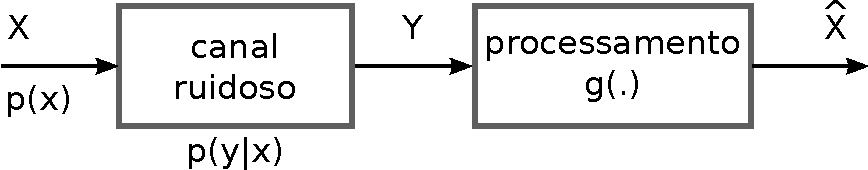
\includegraphics[width=0.7\textwidth]{images/canal-ruidoso.pdf}
  %\caption{.}
  \label{fig:canal-ruidoso}
  \end{figure}

  \begin{itemize}
        \item $\hat{X}$ é uma estimativa de $X$.
        \item a estimativa é errada quando $X \neq \hat{X}$
        \item probabilidade de erro: $P_e \triangleq p(X \neq \hat{X})$
        \item podemos relacionar a entropia condicional $H(X|Y)$ com a probabilidade de erro $P_e$?
        \item sabemos (exercício anterior) que a entropia condicional $H(X|Y)$ é nula se e somente
        se $X$ for uma função de $Y$
        \item esperamos ser capazes de estimar $X$ com baixa probabilidade de erro apenas quando
        a entropia condicional $H(X|Y)$ for pequena
  \end{itemize}
\end{frame}

\subsection{Desigualdade de Fano}

\begin{frame}%[allowframebreaks]
  \frametitle{Desigualdade de Fano}
  \begin{theorem}[Desigualdade de Fano]
  Para qualquer estimador $\hat{X}$ tal que $X \rightarrow Y \rightarrow \hat{X}$, com
  $P_e = Pr(X \neq \hat{X})$, temos
  \begin{equation}
        H(P_e) + P_e \log \left( \vert \mathcal{X} \vert - 1 \right) \geq H(X|\hat{X}) \geq H(X|Y)
  \end{equation}
  Esta desigualdade pode ser simplificada (menos rígida) na forma
  \begin{equation}
  P_e \geq \frac{H(X|Y) - 1}{\log \left( \vert \mathcal{X} \vert - 1 \right)}
  \label{eq:desfanorelax}
  \end{equation}
  onde utilizamos $H(P_e) \leq 1$.
  \end{theorem}
  Note que $P_e = 0 \Rightarrow H(X|Y)=0$ pois $H(P_e)=0$ e $H(X|Y) \geq 0$.
\end{frame}
\note{
Esta desigualdade será utilizada para provar o reverso no teorema de codificação
de Shannon, i.e., que qualquer código com probabilidade de erro $\rightarrow 0$,
à medida que o comprimento do bloco cresce, devemos ter uma taxa $R < C$
(a capacidade do canal, a ser definida).

Para o caso de um alfabeto binário ($\vert \mathcal{X} \vert = 2$),
a desigualdade de Fano na forma da Equação \ref{eq:desfanorelax}
não poderá ser aplicada. Devemos então utilizar a forma mais relaxada:
  \begin{equation}
  P_e \geq \frac{H(X|Y) - 1}{\log \left( \vert \mathcal{X} \vert - 1 \right)} 
        > \frac{H(X|Y) - 1}{\log \vert \mathcal{X} \vert }
  \end{equation}

}

\begin{frame}[allowframebreaks]
  \frametitle{Desigualdade de Fano}
  \begin{proof}
        Definir uma função de erro:
        \begin{equation}
        E = \begin{cases} 1 &, \text{ se } \hat{X} \neq X \text{(erro)} \\
                0       &, \text{ se } \hat{X} = X \text{(sem erro)} 
        \end{cases}
        \end{equation}

        \proofbreak

        Utilizando a regra da cadeia temos:
        \vspace{-0.3cm}
        \begin{eqnarray}
        H(E,X|\hat{X}) &=& H(X|\hat{X}) + \underbrace{H(E|X,\hat{X})}_{=0} \nonumber \\
                        &\text{ou}& \nonumber \\
                        &=& \underbrace{H(E|\hat{X})}_{\leq H(E) = H(P_e)} + \underbrace{H(X|E,\hat{X})}_{\leq P_e \log (\vert \mathcal{X} \vert - 1)}
        \end{eqnarray}
        \vspace{-0.3cm}
        \begin{itemize}
        \item O erro é uma função determinística de $X$ e $\hat{X}$, então, sabendo $X$ e $\hat{X}$,
                determinamos $E$. Desta forma: $H(E|X,\hat{X})=0$.
        \item Condicionar só pode reduzir a entropia: $H(E|\hat{X}) \leq H(E) = H(P_e)$.
        \item Veremos abaixo que $H(X|E,\hat{X}) \leq P_e \log (\vert \mathcal{X} \vert - 1)$.
        \end{itemize}

        \proofbreak

        \vspace{-0.3cm}
        \begin{eqnarray}
        H(X|\hat{X},E) &=& p(E=0) \underbrace{H(X|\hat{X},E=0)}_{=0} + p(E=1)H(X|\hat{X},E=1) \nonumber \\
                        &=& (1-P_e) 0 + P_e H(X|\hat{X},E=1) \leq P_e \log (\vert \mathcal{X} \vert - 1) \nonumber
        \end{eqnarray}
        \begin{itemize}
        \item Se não há erro e conhecemos $\hat{X}$, então determinamos $X$. Não existe entropia 
                residual em $X$ quando é dado $\hat{X}$ e $E=0$. Logo $H(X|\hat{X},E=0)=0$.
        \item Se conhecemos $\hat{X}$ e existe um erro ($E=1$), então sabemos que
                $X$ é diferente de $\hat{X}$, logo isto nos deixa com $(\vert \mathcal{X} \vert - 1)$
                alternativas.
        \end{itemize}

        \proofbreak

        Temos então
        \begin{eqnarray}\label{eq-hhpelog}
        H(X|\hat{X}) &=& H(E|\hat{X}) + H(X|E,\hat{X}) \nonumber \\
                &\leq& H(P_e) + P_e \log (\vert \mathcal{X} \vert - 1)
        \end{eqnarray}

        Como $X \rightarrow Y \rightarrow \hat{X}$ é uma cadeia de Markov, podemos utilizar a
        desigualdade de processamento de dados.
        \begin{eqnarray}\label{hxxhxy}
        I(X;Y) &\geq& I(X;\hat{X}) \nonumber \\
        H(X) - H(X|Y) &\geq& H(X) - H(X|\hat{X}) \nonumber \\
        H(X|\hat{X}) &\geq& H(X|Y)
        \end{eqnarray}

        \proofbreak

        Então, utilizando as Equações \ref{eq-hhpelog} e \ref{hxxhxy}, obtemos
        \begin{equation}
        H(P_e) + P_e \log (\vert \mathcal{X} \vert - 1) \geq H(X|\hat{X}) \geq H(X|Y)
        \end{equation}
        
  \end{proof}
\end{frame}

\begin{frame}%[allowframebreaks]
  \frametitle{Desigualdade de Fano - Sumário}
  Considere a seguinte situação: enviamos $X$ através de um canal ruidoso,
  recebemos $Y$ e realizamos algum pós-processamento.
  \begin{figure}[h!]
  \centering
  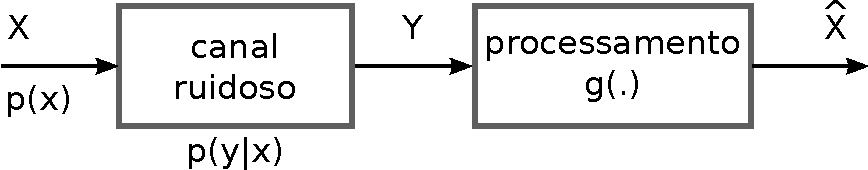
\includegraphics[width=0.8\textwidth]{images/canal-ruidoso.pdf}
  %\caption{.}
  \label{fig:canal-ruidoso}
  \end{figure}
  $\hat{X}$ é uma estimativa de $X$.
  \begin{itemize}
  \item Erro: $X\neq\hat{X}$; com probabilidade $P_e \triangleq p(X\neq \hat{X})$.
  \item Intuitivamente, a entropia condicional deveria nos dizer algo sobre a probabilidade de erro. 
        Na verdade temos o seguinte:
  \end{itemize}

  \begin{theorem}[Desigualdade de Fano]
  \begin{equation}
  H(P_e) + P_e \log (\vert \mathcal{X} \vert -1 ) \geq H(X|\hat{X}) \geq H(X|Y)
  \end{equation}
  \end{theorem}
\end{frame}

\begin{frame}[allowframebreaks]
  \frametitle{Desigualdade de Fano}

  \begin{example}
  Considere uma v.a. discreta $X \in \mathcal{X} = \{1, 2, \ldots, 5\}$ com 
  função massa de probabilidade $p(x) = (0.35, 0.35, 0.1, 0.1, 0.1)$. 
  Seja $Y \in \mathcal{Y} = \{1,2\}$, de forma que, se $x \leq 2$ teremos $y=x$
  com probabilidade $6/7$ e, se $x > 2$, teremos $y=1$ ou $2$ com igual probabilidade.
  A melhor estratégia é utilizar o estimador $\hat{x} = y$. Calcule a probabilidade de erro
  e o limite dado pela desigualdade de Fano.

  \examplebreak

  \textbf{solução}\\
  A distribuição condicional $p(y|x)$ é apresentada na tabela abaixo:
  \begin{center}
  \begin{tabular}{c|cc}
  \diagbox{X}{Y} & 1 & 2 \\
  \hline
  1 & $6/7$  & $1/7$ \\
  2 & $1/7$  & $6/7$ \\
  3 & $1/2$  & $1/2$ \\
  4 & $1/2$  & $1/2$ \\
  5 & $1/2$  & $1/2$
  \end{tabular}
  \end{center}

  \examplebreak

  A efetiva probabilidade de erro é dada por
  \begin{eqnarray}
  P_e &=& 1 - P_a  \ \text{(prob. de acerto)} \nonumber \\
      &=& 1 - \sum_{i=1}^{5} P(x_i = y_i) \nonumber \\
      &=& 1 - \left(  p(y = 1 | x = 1) p(x = 1) + p(y = 2 | x = 2) p(x = 2) + 0 + 0 + 0 \right) \nonumber \\
      &=& 1 - \left( \frac{6}{7} 0.35 + \frac{6}{7} 0.35 \right) = 0.4 = \frac{2}{5}
  \end{eqnarray} 

  \examplebreak

  A desigualdade de Fano fornece um limite inferior pra a probabilidade de erro (predição incorreta do valor de $X$ baseado 
  em $Y$). Este limite inferior é determinado pela incerteza remanescente $H(X|Y)$ sobre $X$ quando $Y$ é conhecido.

  Pelo teorema da desigualdade de Fano temos que
  \begin{equation}
  P_e \geq \frac{H(X|Y) - 1}{\log \left( \vert \mathcal{X} \vert - 1 \right)}
  \end{equation}

  \examplebreak

  Precisaremos calcular 
  \begin{eqnarray}
  H(X|Y) &=& - \sum_{x,y} p(x,y) \log p(x|y) \nonumber \\
         &=& - \sum_{x,y} p(y|x) p(x) \log p(x|y)
  \end{eqnarray}
  onde $p(y|x)$ e $p(x)$ são dados do problema e ainda será necessário calcular $p(x|y)$ para encontrar $H(X|Y)$.

  \examplebreak

  \begin{eqnarray}
  P(X|Y=1) &=& \frac{P(X,Y=1)}{P(Y=1)} = \frac{P(Y=1|X)P(X)}{P(Y=1)} \nonumber \\
        &=& \frac{(\frac{6}{7}, \frac{1}{7}, \frac{1}{2}, \frac{1}{2}, \frac{1}{2}) \cdot (0.35, 0.35, 0.1, 0.1, 0.1) }{ \sum \left( (\frac{6}{7}, \frac{1}{7}, \frac{1}{2}, \frac{1}{2}, \frac{1}{2}) \cdot (0.35, 0.35, 0.1, 0.1, 0.1)  \right)  } \nonumber \\
        &=& \frac{(0.3, 0.05, 0.05, 0.05, 0.05)}{1/2} \nonumber \\
        &=& (0.6, 0.1, 0.1, 0.1, 0.1)
  \end{eqnarray}
  
  \examplebreak

  \begin{eqnarray}
  P(X|Y=2) &=& \frac{(\frac{1}{7}, \frac{6}{7}, \frac{1}{2}, \frac{1}{2}, \frac{1}{2}) \cdot (0.35, 0.35, 0.1, 0.1, 0.1) }{ \sum \left( (\frac{1}{7}, \frac{6}{7}, \frac{1}{2}, \frac{1}{2}, \frac{1}{2}) \cdot (0.35, 0.35, 0.1, 0.1, 0.1)  \right)  } \nonumber \\
        &=& (0.1, 0.6, 0.1, 0.1, 0.1)
  \end{eqnarray}

  \examplebreak 
  
  Desta forma teremos
  \begin{eqnarray}
  H(X|Y) &=& H(X|Y=1) P(Y=1) + H(X|Y=2) P(Y=2) \nonumber \\
        &=& - \frac{1}{2} \left( 0.6 \log 0.6 + 4 \times 0.1 \log 0.1 \right) - \frac{1}{2} \left( 4 \times 0.1 \log 0.1 + 0.6 \log 0.6 \right) \nonumber \\
        &=& 1.771 \text{ bits. }
  \end{eqnarray}

  Utilizando a desigualdade de Fano
  \begin{eqnarray}
  P_e &\geq& \frac{H(X|Y) - 1}{\log \left( \vert \mathcal{X} \vert -1 \right)} = \frac{1.771 - 1}{ \log (5-1)} = 0.3855
  \end{eqnarray}

  \end{example}
\end{frame}

\begin{frame}[allowframebreaks]
  \frametitle{Desigualdade de Fano}
  \begin{lemma}
  Se $X$ e $X'$ são i.i.d. com entropia $H(X)$,
        \begin{equation}
        Pr(X = X') \geq 2^{-H(X)}
        \end{equation}
  com igualdade se e somente se $X$ possuir distribuição uniforme.
  \end{lemma}

  \begin{eqnarray}
  Pr(X = X') &=& Pr(X=x_1|X'=x_1)Pr(X'=x_1) + \ldots + \nonumber \\ && Pr(X=x_n|X'=x_n)Pr(X'=x_n) \nonumber \\
        &=& Pr(X=x_1)Pr(X'=x_1) + \ldots + \nonumber \\ && Pr(X=x_n)Pr(X'=x_n) \nonumber \\
        &=& p^2(x_1) + \ldots + p^2(x_n) = \sum_x p^2(x)
  \end{eqnarray}

  \framebreak

  \begin{proof}
  Suponha que $X \sim p(x)$. Pela desigualdade de Jensen temos
        \begin{equation}
        2^{E[\log p(X)]} \leq E[2^{\log p(X)}]
        \end{equation}
  pois $2^x$ é convexa.
  Logo,
        \begin{eqnarray}
        2^{-H(X)} &=& 2^{\sum_x p(x) \log p(x)} = 2^{E[\log p(X)]} \nonumber \\
                &\leq& E[2^{\log p(X)}] \nonumber \\
                &=& \sum_x p(x) 2^{\log p(x)} = \sum_x p(x)p(x) \nonumber \\
                &=& \sum_x p^2(x) = Pr(X = X')
        \end{eqnarray}
  \end{proof}

  \framebreak
  
  Note que, para maximizar a probabilidade $Pr(X = X')$, devemos minimizar a entropia.
  No limite, quando $H(X)=0$, teremos $Pr(X = X') \geq 1$, logo será igual a $1$ e assim $X = X'$ sem dúvida.
\end{frame}

\begin{frame}[allowframebreaks]
  \frametitle{Desigualdade de Fano}
  \begin{corollary}
  Seja $X, X'$ independentes com $X \sim p(x)$ e $X' \sim q(x)$, $x,x' \in \mathcal{X}$, então
  \begin{eqnarray}
  Pr(X=X') \geq 2^{-H(p) - D(p||q)} \nonumber \\
  Pr(X=X') \geq 2^{-H(q) - D(q||p)}
  \end{eqnarray} 
  ou seja
  \begin{equation}
  Pr(X=X') \geq \max \left( 2^{-H(p) - D(p||q)} , 2^{-H(q)-D(q||p)} \right)
  \end{equation}
  \end{corollary}

  \framebreak

  \begin{proof}
        \begin{eqnarray}
        2^{-H(p) - D(p||q)} &=& 2^{\sum_x p(x) \log p(x) + \sum_x p(x) \log \frac{q(x)}{p(x)}} \nonumber \\
                &=& 2^{\sum_x p(x) \log q(x)} \nonumber \\
                &=& 2^{E_p[\log q(X)]} \nonumber \\
                &\leq& \sum_x p(x) 2^{\log q(x)}  \text{ (Jensen)} \nonumber \\
                &=& \sum_x p(x) q(x) \nonumber \\
                &=& Pr(X=X')
        \end{eqnarray}
  \end{proof}
\end{frame}


% propriedade da equipartição assintótica / conjunto típico
\section{Propriedade da Equipartição Assintótica}

\begin{frame}%[allowframebreaks]
  \frametitle{Propriedade da Equipartição Assintótica}
  \begin{itemize}
  \item Vamos considerar blocos de realizações de uma variável aleatória 
        (i.e., vetores aleatórios de comprimento $n$). $n = \text{tamanho do bloco}$.
  \item Sejam $X_1, X_2, \ldots, X_n$ v.a.s i.i.d. com distribuição $p$ (dizemos
        $X_i \sim p(x)$).
  \item Existem $K$ símbolos possíveis (alfabeto ou espaço-estado de tamanho $K$), então
        $X_i \in \{a_1, a_2, \ldots, a_K\}$.
  \item Consideram $n$ variáveis aleatórias $(X_1, X_2, \ldots, X_n)$, existem $K^n$ possíveis
        realizações.
  \end{itemize}
\end{frame}


\begin{frame}%[allowframebreaks]
  \frametitle{Propriedade da Equipartição Assintótica}
  Suponha que desejamos codificar as $K^n$ possíveis realizações com uma sequência de
  dígitos binários de comprimento $m$. Então, existem $2^m$ palavras de código (\textit{codewords}).
  
  \begin{figure}[h!]
  \centering
  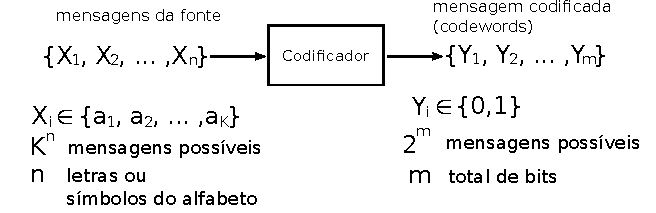
\includegraphics[width=0.7\textwidth]{images/blockcoding.pdf}
  %\caption{.}
  \label{fig:blockcoding}
  \end{figure}
 
  \begin{itemize}
  \item Para que seja possível termos uma palavra de código para cada mensagem possível,
  devemos satisfazer a seguinte condição:
        \begin{equation}
        2^m \geq K^n
        \end{equation}
        ou seja
        \begin{equation}
        m \geq (\log K) n
        \end{equation}
  \end{itemize}
\end{frame}


\begin{frame}%[allowframebreaks]
  \frametitle{Propriedade da Equipartição Assintótica}
  \begin{itemize}
  \item Quantos bits por letra da fonte utilizamos?
        \begin{equation}
        \text{taxa} = \frac{m}{n} \geq \log K \text{ bits por letra da fonte}
        \end{equation}
        Exemplo: 26 letras, precisaremos de $\lceil \log K \rceil = 5 \text{bits}$.
  \item Podemos utilizar menos bits por símbolo emitido pela fonte (na média) e ainda sim
        não ter erro? Sim.
  \item Algumas mensagens da fonte poderiam não ter a elas um código associado.

  \begin{figure}[h!]
  \centering
  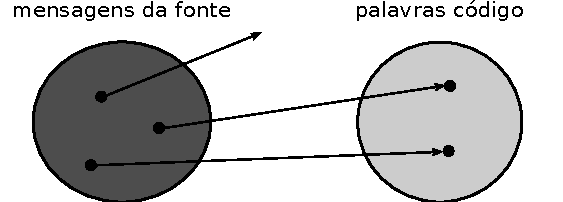
\includegraphics[width=0.5\textwidth]{images/cword-map.pdf}
  %\caption{.}
  \label{fig:cword-map}
  \end{figure}

  \end{itemize}
\end{frame}


\begin{frame}%[allowframebreaks]
  \frametitle{Propriedade da Equipartição Assintótica}
  \begin{itemize}
  \item Ao invés de descartar algumas mensagens, podemos associar a elas palavras longas
        e às outras palavras associamos palavras curtas.

  \begin{figure}[h!]
  \centering   
  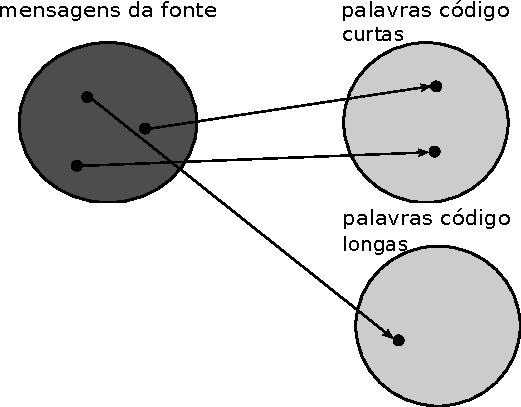
\includegraphics[width=0.35\textwidth]{images/cword-map2.pdf}
  %\caption{.}
  \label{fig:cword-map}
  \end{figure}

  \item Em qualquer um dos casos, quando $n$ é grande suficiente, podemos fazer com que a
        probabilidade, de se obter uma dessas mensagens da fonte que gerariam erro 
        (ou que teriam palavras longas associadas), muito pequena.

  \end{itemize}
\end{frame}


\begin{frame}%[allowframebreaks]
  \frametitle{Probabilidade de Palavras da Fonte}
  \begin{itemize}
  \item A probabilidade de palavras da fonte i.i.d. pode ser expressa por
        \begin{equation}
        p(X_1 = x_1, X_2 = x_2, \ldots, X_n = x_n) = \prod_{i=1}^{n} p(X_i = x_i)
        \end{equation}
  \item A informação (Shannon/Hartley) sobre um evento é dada por $-\log p(x) = I(x)$, então
        \begin{eqnarray}
        I(x_1,x_2,\ldots,x_n) &=& - \log p(x_1, x_2, \ldots, x_n) = - \log \prod_{i=1}^n p(x_i) \nonumber \\
                        &=& \sum_{i=1}^n - \log p(x_i) = \sum_{i=1}^n I(x_i)
        \end{eqnarray}
  \item Eventos independentes são aditivos em relação a esta função de informação.
  \item Note que: $E I(X) = H(X)$.
  \item A lei fraca dos grandes números diz que $\frac{1}{n} S_n \xrightarrow{p} \mu$, onde $S_n$ é a soma
        de v.a.s i.i.d. com média $\mu = E X_i$.
  \item $I(X_i)$ também é uma v.a. com média $H(X)$.
  \end{itemize}
\end{frame}
\note{
\textbf{Lei dos Grandes Números}

Se um evento de probabilidade $p$ é observado repetidamente em ocasiões independentes, 
a proporção da frequência observada deste evento em relação ao total número de repetições 
converge em direção a $p$ à medida que o número de repetições se torna arbitrariamente grande.

\vspace{1cm}

Sejam $X_1, X_2, \ldots, X_n$ v.a.s i.i.d. com $\E X_i = \mu$ e $\Var X_i = \sigma^2 < \infty$, para $i=1,\ldots,n$.
Seja a média definida por $\overline{X_n} = \frac{1}{n} \sum_{i=1}^{n} X_i$, então, para $\varepsilon > 0$,
a \textbf{Lei Fraca dos Grandes Números} diz que $\overline{X_n}$ converge em probabilidade para $\mu$, ou seja,
\begin{equation}
\lim_{n \rightarrow \infty} P \left( \vert \overline{X_n} - \mu \vert < \varepsilon  \right) = 1 .
\end{equation}
}

\begin{frame}%[allowframebreaks]
  \frametitle{Lei fraca dos grandes números e Entropia}
  \begin{itemize}
  \item Combinando o que vimos anteriormente, obtemos
        \begin{equation}
        \frac{1}{n} \sum_{i=1}^n I(X_i) \xrightarrow[n \rightarrow \infty]{p} H(X)
        \end{equation}
  \item Se $n$ fica grande suficiente, obteremos
        \begin{eqnarray}
        \frac{1}{n} \sum_{i=1}^n I(x_i) &\approx& H(X) \text{ onde } \forall i, x_i \sim p(x) \nonumber \\
        - \frac{1}{n} \sum_{i=1}^n \log p(x_i) &\approx& H(X) \nonumber \\
        - \log \prod_{i=1}^n p(x_i) &\approx& n H(X) \nonumber \\
        - \log p(x_1,x_2,\ldots,x_n) &\approx& n H(X) \nonumber \\
        p(x_1,x_2,\ldots,x_n) &\approx& 2^{-nH(X)}
        \end{eqnarray}
  \end{itemize}
\end{frame}

\begin{frame}%[allowframebreaks]
  \frametitle{Propriedade da Equipartição Assintótica}
        Quando $n$ é grande suficiente, teremos
        \begin{equation}
        p(x_1,x_2,\ldots,x_n) \approx 2^{-nH(X)}
        \end{equation}
        
        \begin{itemize}
        \item Esta probabilidade não depende da sequência em si. Depende apenas do comprimento $n$
        e da entropia da v.a.
        \item Quando $n$ fica grande, podemos dizer que todas as sequências terão a mesma probabilidade: $2^{-nH}$.
        \item Estas sequências que possuem esta probabilidade (praticamente todas as sequências) são
        chamadas de sequências \textbf{típicas}, e são representadas pela conjunto $A$.
        \end{itemize}
\end{frame}

\begin{frame}%[allowframebreaks]
  \frametitle{Quase todos eventos são quase equiprováveis}
  \begin{itemize}
  \item Se $X_1,X_2,\ldots,X_n$ são i.i.d. e $X_i \sim p(x)$ para todo $i$, e se $n$ é grande suficiente, 
        então qualquer amostra $x_1,x_2,\ldots,x_n$ terá 
        probabilidade da amostra essencialmente independente da amostra, i.e.,
        \begin{equation}
        p(x_1,\ldots,x_n) \approx 2^{-nH(X)}
        \end{equation}
        onde $H(X)$ é a entropia de $p(x)$.
  \item Então, podem existir no máximo $2^{nH}$ amostras, e pode ser que $2^{nH} \ll K^n$.
  \item Estas amostras que ocorrem são chamadas de típicas, e são representadas por $A_\epsilon^{(n)}$.
  \item Uma grande porção de $\mathcal{X}^n$ não irá ocorrer, i.e., pode acontecer que 
        $2^{nH} \ll \vert \mathcal{X}^n \vert = K^n$.
  \end{itemize}
\end{frame}

\begin{frame}%[allowframebreaks]
  \frametitle{Conjunto Típico}
  \begin{itemize}
  \item Seja $A_\epsilon^{(n)}$ o conjunto das sequências típicas (i.e., aquelas com probabilidade $2^{-nH}$).
  \item Se ``todos'' eventos possuem a mesma probabilidade $p$, então existem $1/p$ deles.
  \item O número de sequências típicas é
        \begin{equation}
        \vert A_\epsilon^{(n)} \vert \approx 2^{nH(X)}.
        \end{equation}
  \item Desta forma, para representar (ou codificar) as sequencias típicas, precisaremos de
        $nH(X)$ bits. Teremos então
        \begin{equation}
        m = nH(X)
        \end{equation}
        no modelo do codificador. Então a taxa será $H(X)$.
  \end{itemize}

\end{frame}


\begin{frame}%[allowframebreaks]
  \frametitle{Codificando apenas o Conjunto Típico}
  \begin{itemize}
  \item Tomando $m=nH$, teremos que o número médio de bits por letra do alfabeto da fonte será dado por
        \begin{equation}
        \frac{m}{n} = H         \text{  que pode ser } \leq \log K
        \end{equation}
  \item Interpretações para a Entropia na codificação de fonte:
        \begin{enumerate}
        \item A probabilidade de uma sequência típica é $2^{-nH(X)}$.
        \item O número de sequências típicas é $2^{nH(X)}$.
        \item O número de bits por símbolo da fonte é $H(X)$, quando codificamos apenas o conjunto típico.
        \end{enumerate}
  \end{itemize}
\end{frame}


\begin{frame}%[allowframebreaks]
  \frametitle{Bernoulli}
  Considere o experimento de Bernoulli com $X_1,\ldots,X_n$ i.i.d. e probabilidade
  $p(X_i=1)=p=1-p(X_i=0)$. A probabilidade de uma dada sequência será dada por
  \begin{equation}
  p(x_1,x_2,\ldots,x_n) = \prod_{i=1}^n p^{x_i} (1-p)^{1-x_i} = p^{\sum_i x_i} (1-p)^{n - \sum_i x_i}
  \end{equation}

  \begin{itemize}
  \item Existem $2^n$ sequencias possíveis.
  \item Todas elas possuem a mesma probabilidade? Não. Considere $p=0.1$, $(1-p)=0.9$.
        A sequência de apenas zeros é a sequência de mais provável.
  %\item Qual é a sequência mais provável? Quando $p=0.1$, será a sequência com apenas zeros.
  \end{itemize}
\end{frame}
\note{
  Todas as sequências que possuem `alguma' probabilidade, terão a mesma probabilidade?
  Depende do que queremos dizer com `alguma'. Para valores pequenos de $n$, não, mas à medida
  que $n$ cresce, algo acontece e a resposta `sim' começa a ser a mais apropriada. 
}

\begin{frame}%[allowframebreaks]
  \frametitle{Propriedade de Equipartição Assintótica}
  \begin{itemize}
  \item É possível prever a probabilidade de que uma determinada sequências terá uma probabilidade particular?
        \begin{equation}
        \Pr(p(X_1,X_2,\ldots,X_n)=\alpha) = ?
        \end{equation}
  \item Note que $p(X_1,X_2,\ldots,X_n)$ é uma variável aleatória. É uma probabilidade que é uma função
        do conjunto de variáveis aleatórias.
  \item Teremos
        \begin{equation}
        \Pr(p(X_1,X_2,\ldots,X_n) \approx 2^{-nH} ) \approx 1
        \end{equation}
        quando $n$ é grande suficiente.
  \item Quase todos os eventos (que ocorrem com alguma probabilidade) são todos equiprováveis.
  \end{itemize}
\end{frame}

\begin{frame}%[allowframebreaks]
  \frametitle{Ensaio de Bernoulli}
  \begin{example}
  Seja $S_n \sim \text{Binomial}(n,p)$ com $S_n = X_1 + X_2 + \ldots + X_n$, $X_i \sim \text{Bernoulli}(p)$.
  Teremos então $ES_n = np$ e $\text{var}(S)=npq$, onde $q=1-p$, e
        \begin{equation}
        p(S_n = k) = {n \choose k} p^k q^{n-k}
        \end{equation}
  Analisando a expressão para $2^{-nH}$, temos
        \begin{eqnarray}
        2^{-nH(p)} &=& 2^{-n(-p \log p - (1-p)\log(1-p))} \nonumber \\
                &=& 2^{\log p^{np} + \log(1-p)^{n(1-p)}} \nonumber \\
                &=& p^{np}q^{nq}
        \end{eqnarray}
  $H=H(p)$ é a entropia binária com probabilidade $p$.
  $np$ é o número esperado de $1$s e $nq$ é o número esperado de $0$s.
  \end{example}
\end{frame}
\note{
        \begin{itemize}
        \item Todas as sequências que ocorrem são aquelas cujo número de $1$s e $0$s são
                aproximadamente iguais aos seus valores esperados.
        \item Nenhum outra sequência possui probabilidade significativa.
        \item A sequência $X_1, X_2, \ldots, X_n$ foi assumida como sendo i.i.d., entretanto
                podemos estender para cadeias de Markov e processos aleatórios estacionários ergódicos.
        \end{itemize}
}
\note{
O cálculo computacional do coeficiente binomial pode apresentar perda de precisão numérica, por envolver
fatoriais e frações de números muito grandes. Exemplo de execussão no GNU-Octave para calcular ${100 \choose 20}$:
\begin{semiverbatim}
>> nchoosek(100,20)

warning: nchoosek: possible loss of precision

warning: called from
\end{semiverbatim}
Uma possível solução é utilizar o pacote simbólico para efetuar os cálculos. 
Podemos verificar que realmente ocorreu erro de precisão numérica ao realizar o cálculo computacional.
\begin{semiverbatim}
>> double(nchoosek(sym(100),sym(20))) - nchoosek(100,20)

ans = -65536
\end{semiverbatim}
}
\note{
Outra alternativa é realizar uma aproximação para calcular ${N \choose k}$.

Iremos utilizar a aproximação de Stirling para a função fatorial:
\begin{equation}
\ln n! =  n \ln n - n + \mathcal{O}(\ln n) 
\end{equation}
%\begin{equation}
%\ln x! \simeq x \ln x - x + \frac{1}{2} \ln 2 \pi x .
%\end{equation}
Utilizando esta aproximação em $\ln {N \choose k}$, teremos
\begin{eqnarray}
\ln {N \choose k} &\equiv& \ln \frac{N!}{(N-k)!k!} = \ln N! - \ln (N-k)! - \ln k! \nonumber \\
        &\simeq& N \ln N - N - (N-k) \ln (N-k) + (N-k) - k \ln k + k \nonumber \\
        &=& \underbrace{(N-k)\ln N - (N-k)\ln N}_{=0} + N \ln N - N - (N-k) \ln (N-k) + (N-k) - k \ln k + k \nonumber \\
        &=& (N-k)\ln \frac{N}{N-k} + k \ln \frac{N}{k}  \nonumber \\
        &=& N \left( -\frac{N-k}{N} \ln \frac{N-k}{k} - \frac{k}{N} \ln \frac{k}{N} \right) = N H_e\left(\frac{k}{N}\right) .
%\frac{N \ln N - N + \frac{1}{2} \ln 2\pi N}{ \left( (N-k) \ln (N-k) - (N-k) + \frac{1}{2} \ln 2\pi (N - k) \right) \left( k \ln k - k + \frac{1}{2} \ln 2\pi k \right) }
\end{eqnarray}
}
\note{
Concluímos então que
\begin{equation}
\ln {N \choose k} \simeq N H_e\left(\frac{k}{N}\right)
\end{equation}
e, como os temos em ambos os lados envolvem logaritmos, podemos realizar a mudança de base em ambos os lados
(basta multiplicar por $\ln 2$),
\begin{equation}
\log {N \choose k} \simeq N H \left(\frac{k}{N}\right) ,
\end{equation}
onde agora utilizamos a entropia binária em bits. Assim, teremos
\begin{equation}
{N \choose k} \simeq 2^{N H \left(\frac{k}{N}\right)} .
\end{equation}

}


\begin{frame}%[allowframebreaks]
  \frametitle{Propriedade da Equipartição Assintótica}
  \begin{theorem}[Propriedade da Equipartição Assintótica]\label{thm-prop-eqp-ass}
        Se $X_1, X_2, \ldots, X_n$ são i.i.d. e $X_i \sim p(x)$ para todo $i$, então
        \begin{equation}\label{eq-pX1X2Xn-H}
        -\frac{1}{n} \log p(X_1, X_2, \ldots, X_n) \xrightarrow{p} H(X)
        \end{equation}
  \end{theorem}

  \begin{proof}
  \vspace{-2ex}
  \begin{eqnarray}
  -\frac{1}{n} \log p(X_1, X_2, \ldots, X_n) &=& - \frac{1}{n} \log \prod_{i=1}^n p(X_i) \nonumber \\
                &=& - \frac{1}{n} \sum_i \log p(X_i) \xrightarrow{p} E \log p(X) \nonumber \\
                && \text{\scriptsize onde utilizamos a lei fraca dos números grandes} \nonumber \\
                &=& H(X)
  \end{eqnarray}
  \end{proof}
\end{frame}


\begin{frame}%[allowframebreaks]
  \frametitle{Conjunto Típico}
  \begin{definition}[Conjunto Típico]
  Um conjunto típico $A_\epsilon^{(n)}$ em relação a $p(x)$ é o conjunto de sequências 
  $(x_1,x_2,\ldots,x_n) \in \mathcal{X}^n$ com propriedade
        \begin{equation}
        2^{-n(H(X)+\epsilon)} \leq p(x_1, x_2, \ldots, x_n) \leq 2^{-n(H(X)-\epsilon)}
        \end{equation}
  De forma equivalente, podemos escrever
        \begin{equation}
        A_\epsilon^{(n)} = \left\{ (x_1, x_2, \ldots, x_n) : \vert - \frac{1}{n} \log p(x_1, \ldots, x_n) - H \vert < \epsilon \right\}
        \end{equation}
  \end{definition}

  O conjunto típico é formado pelas sequências com $\log$ da probabilidade dentro
  de seguinte extensão 
  \begin{figure}[h!]
  \centering
  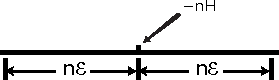
\includegraphics[width=0.35\textwidth]{images/range-ts.pdf}
  %\caption{.}
  \label{fig:range-ts}
  \end{figure}
\end{frame}


\begin{frame}%[allowframebreaks]
  \frametitle{Conjunto Típico}
  \begin{itemize}
  \item O tamanho do conjunto típico de sequências produzidas pela fonte é tipicamente
        muito menor que o tamanho do conjunto de todas as sequências produzidas pela fonte.
  \item Uma sequencia típica não precisa ter probabilidade próxima daquela que é a sequência mais provável.
  \item Geralmente a sequência mais provável não está no conjunto típico.
  \end{itemize}
\end{frame}



\subsection{Propriedades do Conjunto Típico}
\begin{frame}%[allowframebreaks]
  \frametitle{Propriedades do Conjunto Típico}
  \begin{theorem}[Propriedades do Conjunto Típico $A_\epsilon^{(n)}$]
  \begin{enumerate}
  \item Se $(x_1, x_2, \ldots, x_n) \in A_\epsilon^{(n)}$, então
        \begin{equation}
        H(X) - \epsilon \leq - \frac{1}{n} \log p(x_1, x_2, \ldots, x_n) \leq H(X) + \epsilon
        \end{equation}
  \item $p(A_\epsilon^{(n)}) = p\left( \left\{ x: x \in A_\epsilon^{(n)} \right\} \right) > 1 - \epsilon$ para $n$ grande suficiente, para todo $\epsilon > 0$.
  \item Limite superior: $\vert A_\epsilon^{(n)} \vert \leq 2^{n(H(X)+\epsilon)}$, onde $\vert A_\epsilon^{(n)} \vert$ é o número de elementos no conjunto $A_\epsilon^{(n)}$.
  \item Limite inferior: $\vert A_\epsilon^{(n)} \vert \geq (1-\epsilon) 2^{n(H(X) - \epsilon)}$ para $n$ grande suficiente.
  \end{enumerate}
  \end{theorem}

  \begin{itemize}
  \item O conjunto típico possui, essencialmente, probabilidade $1$ (algo típico irá tipicamente ocorrer).
  \item Todos os itens neste conjunto terão a mesma probabilidade $\approx 2^{-nH}$.
  \end{itemize}
\end{frame}

\begin{frame}%[allowframebreaks]
  \frametitle{Exemplo $K=\vert \{0,1\} \vert$: Conjunto Típico}
  \begin{itemize}
  \item Suponha o Ensaio de Bernoulli com distribuição uniforme, $K=2$, 
        $\mathcal{X} = \{0,1\}$, $p=0.5$, entropia $H=1$ e
        $\vert A_\epsilon^{(n)} \vert = 2^{nH} = 2^n = K^n$, 
        então todas as sequências ocorreram com igual probabilidade.
  \item Considere agora uma distribuição não-uniforme, $p=0.1$ e $q=1-p=0.9$, a entropia será
        $H\approx 0.469$. Considere $n=100$, então 
        $K^{100} = 2^{100} = 10^{\log_{10} 2^{100}} \approx 10^{100 \times 0.30103} \approx 10^{30}$,
        a capacidade representacional das sequencias da fonte. 
        Mas $\vert A_\epsilon^{(n)} \vert = 2^{nH} = 10^{nH \times \log_{10} 2} \approx 10^{14} \ll 10^{30} \approx K^{100}$. 
        O número de sequências típicas é muito menor que o número de possíveis sequências.
  \item Ineficiência: capacidade representacional é muito maior do que as coisas que ocorrem.
        O alfabeto da fonte é pobre para realizar compressão.
  \item Assuma $\epsilon$ muito pequeno, então onde foi parar a massa das $\approx 10^{30} - 10^{14}$ 
        sequencias? (veremos adiante)
  \end{itemize}
\end{frame}


\begin{frame}%[allowframebreaks]
  \frametitle{Conjunto Típicos são Típicos}
  \begin{itemize}
  \item Pela definição
        \begin{equation}
        p(A_\epsilon^{(n)}) > 1 - \epsilon \text{ para qualquer } \epsilon > 0
        \end{equation}
  \item Então $A_\epsilon^{(n)}$ possui praticamente toda probabilidade, e cada elemento
        em $A_\epsilon^{(n)}$ possui a mesma probabilidade, então
        \begin{equation}
        p(x) \approx 2^{-nH} \forall x \in A_\epsilon^{(n)}
        \end{equation}
  \item Exemplo: Ensaio de Bernoulli $X_i \sim \text{Bernoulli}(p)$ com 
        $p(X_i = 1) = p = 1 - p(X_i = 0)$ e $p>0.5$.
  \item Probabilidade de $n$ $1$s sucessivos é $p^n$ e esta é a sequência mais provável.
  \item Probabilidade de uma sequência típica é $2^{-nH}$.
  \item Para $n=100$, $p-0.9 = 1 - q$, a sequência mais provável possui probabilidade
        $p^n \approx 2.66 \times 10^{-5}$, mas uma sequencia típica possui probabilidade
        $2^{-nH} \approx 7.62 \times 10^{-15}$.
  \end{itemize}
\end{frame}

\begin{frame}%[allowframebreaks]
  \frametitle{Exemplo $K=\vert \{0,1\} \vert$: Conjunto Típico}
  \begin{itemize}
  \item Suponha o Ensaio de Bernoulli com distribuição uniforme, $K=2$, 
        $\mathcal{X} = \{0,1\}$, $p=0.5$, entropia $H=1$ e
        $\vert A_\epsilon^{(n)} \vert = 2^{nH} = 2^n = K^n$, 
        então todas as sequências ocorreram com igual probabilidade.
  \item Considere agora uma distribuição não-uniforme, $p=0.1$ e $q=1-p=0.9$, a entropia será
        $H\approx 0.469$. Considere $n=100$, então 
        $K^{100} = 2^{100} = 10^{\log_{10} 2^{100}} \approx 10^{100 \times 0.30103} \approx 10^{30}$,
        a capacidade representacional das sequencias da fonte. 
        Mas $\vert A_\epsilon^{(n)} \vert = 2^{nH} = 10^{nH \times \log_{10} 2} \approx 10^{14} \ll 10^{30} \approx K^{100}$. 
        O número de sequências típicas é muito menor que o número de possíveis sequências.
  \item Ineficiência: capacidade representacional é muito maior do que as coisas que ocorrem.
        O alfabeto da fonte é pobre para realizar compressão.
  \item Assuma $\epsilon$ muito pequeno, então onde foi parar a massa das $\approx 10^{30} - 10^{14}$ 
        sequencias? (veremos adiante)
  \end{itemize}
\end{frame}

\begin{frame}%[allowframebreaks]
  \frametitle{Conjunto Típicos são Típicos}
  \begin{itemize}
  \item Pela definição
        \begin{equation}
        p(A_\epsilon^{(n)}) > 1 - \epsilon \text{ para qualquer } \epsilon > 0
        \end{equation}
  \item Então $A_\epsilon^{(n)}$ possui praticamente toda probabilidade, e cada elemento
        em $A_\epsilon^{(n)}$ possui a mesma probabilidade, então
        \begin{equation}
        p(x) \approx 2^{-nH} \forall x \in A_\epsilon^{(n)}
        \end{equation}
  \item Exemplo: Ensaio de Bernoulli $X_i \sim \text{Bernoulli}(p)$ com 
        $p(X_i = 1) = p = 1 - p(X_i = 0)$ e $p>0.5$.
  \item Probabilidade de $n$ $1$s sucessivos é $p^n$ e esta é a sequência mais provável.
  \item Probabilidade de uma sequência típica é $2^{-nH}$.
  \item Para $n=100$, $p-0.9 = 1 - q$, a sequência mais provável possui probabilidade
        $p^n \approx 2.66 \times 10^{-5}$, mas uma sequencia típica possui probabilidade
        $2^{-nH} \approx 7.62 \times 10^{-15}$.
  \end{itemize}
\end{frame}

\begin{frame}%[allowframebreaks]
  \frametitle{Sequencias Não-Típicas não são típicas}
  \begin{itemize}
  \item $p^n \gg 2^{-nH}$: a sequência mais provável é muito mais provável do que uma 
        sequencia típica.
  \item O que ocorre com a probabilidade da sequencia mais provável, na média (por símbolo),
        quando $n$ cresce
        \begin{equation}
        - \frac{1}{n} \log p^n = - \log p = \log 1/p \xrightarrow[n \rightarrow \infty] p H ?
        \end{equation} 
  \item O conjunto típico possui, essencialmente, toda a probabilidade $p(A_\epsilon^{(n)}) > 1 - \epsilon $.
  \item A sequencia mais provável está no conjunto típico? 
        Não, já que a probabilidade da sequencia mais provável não é $2^{-nH}$.
  \item $n=100$, $p=0.9=1-q$. Considere uma sequência com noventa $1$s e dez $0$s.
        A probabilidade é $p^{90}(1-p)^{10} \approx 7.62 \times 10^{-15} \approx 2^{-nH}$.
  \item Esta sequencia muito improvável é típica.
  \end{itemize}
\end{frame}

\begin{frame}%[allowframebreaks]
  \frametitle{Probabilidade Média de Sequencias}
  \begin{itemize}
  \item Pela PEA (Propriedade da Equipartição Assintótica), temos que se 
        $(x_1, \ldots, x_n)$ é típico (i.e., $(x_1, \ldots, x_n) \in A_\epsilon^{(n)}$, 
        para qualquer $\epsilon > 0$), então
        \begin{equation}
        - \frac{1}{n} \log p(x_1, \ldots, x_n) \xrightarrow[n \rightarrow \infty]{p} H 
        \end{equation}
  \item Para as sequencias mais prováveis, quando $n$ é grande suficiente, teremos (para $p>0.5$)
        \begin{equation}
        - \frac{1}{n} \log p^n = - \log p = \log 1/p \xrightarrow[n \rightarrow \infty]{p} - \log p
        \end{equation}
  \item A probabilidade média da sequencia mais provável é bem diferente da sequencia típica.
  \end{itemize}
\end{frame}

\begin{frame}%[allowframebreaks]
  \frametitle{Sequencias Típicas}
  \begin{itemize}
  \item o conjunto típico possui essencialmente toda da probabilidade.
  \item Como pode uma sequencia com a maior probabilidade não ser típica,
        mas uma sequência com probabilidade muito menor ser típica?
  \item Existe um número exponencialmente crescente de sequencias típicas, cada uma
        com probabilidade menor do que a sequencia de maior probabilidade.
  \item A probabilidade individual de cada sequencia vai a zero quando $n$ cresce.
  \item O tamanho do conjunto típico cresce rapidamente, quando $n \rightarrow \infty$,
        de forma que a probabilidade de $A_\epsilon^{(n)}$ vai a $1$.
  \item O tamanho do conjunto das sequencias muito prováveis cresce lentamente, de forma
        que a probabilidade do conjunto vai a zero quando $n \rightarrow \infty$. 
  \end{itemize}
\end{frame}

\begin{frame}[allowframebreaks]
  \frametitle{Sequencias Típicas} 
  A probabilidade de uma sequência $x_{1:n}$, onde $x_i \in \mathcal{X} = \{a_1, \ldots, a_K\}$, é dada por
  \begin{equation}
  P(x_{1:n}) = P(x_1) P(x_2) \ldots P(x_n) \approx p_1^{p_1 n} p_2^{p_2 n} \ldots p_K^{p_K n} ,
  \end{equation}
  onde consideramos que, em uma sequência muito longa, esperamos observar $p_1 n$ ocorrências do símbolo $a_1$,
  $p_2 n$ ocorrências do símbolo $a_2$, etc.

  A informação associada a esta sequência típica é
  \begin{eqnarray}
  \log \frac{1}{P(x_{1:n})} &\approx& \sum_{i=1}^K \log p_i^{-p_i n} \\
                &=& n \sum_{i=1}^K p_i \log \frac{1}{p_i} = n H(X).
  \end{eqnarray}
  Uma sequência típica terá probabilidade próxima de $2^{-n H(X)}$.

  \framebreak
  \begin{figure}[h!]
  \centering
  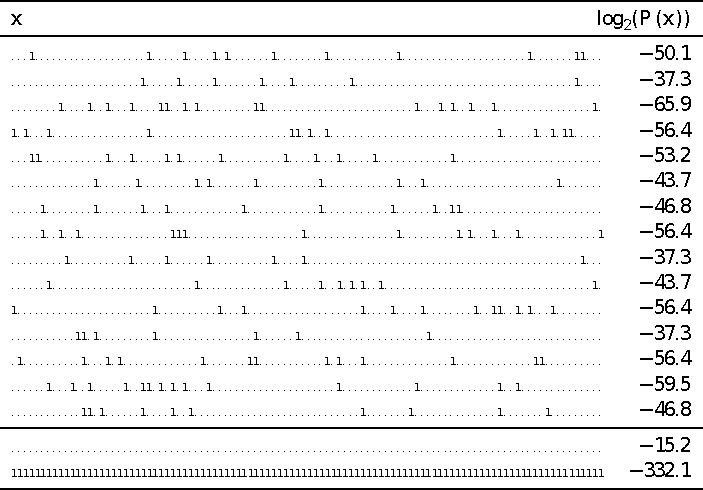
\includegraphics[width=0.5\textwidth]{images/seq100mackay.pdf}
  \caption{Sequências regadas por um ensaio de Bernoulli com $n=100$ e $P(X=1) = p = 0.1$. 
        As 15 sequências superiores representam amostras típicas. As duas últimas sequências
        representam a sequência mais provável e a menos provável \cite{mackay2003}.}
  \label{fig:seq100mackay}
  \end{figure}

  \framebreak
  \begin{figure}[h!]
  \centering
  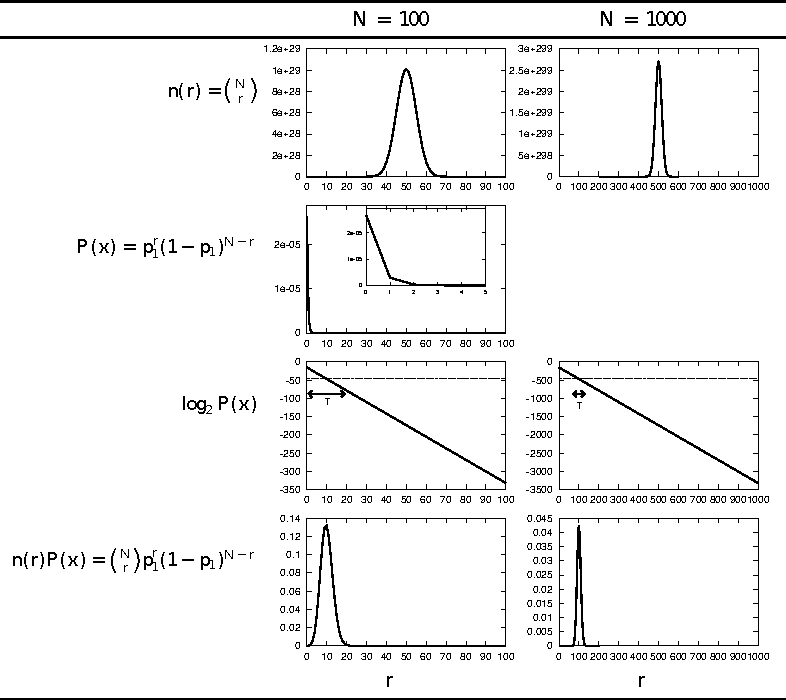
\includegraphics[width=0.5\textwidth]{images/seq100mackay2.pdf}
  \caption{Para $p=0.1$, $n=100$ e $n=1000$ os gráficos ilustram $n(r)$, o número de strings contendo
        $r$ 1s; a probabilidade $P(x_{1:n})$ para uma string contendo $r$ 1s; a mesma probabilidade
        em escala logarítmica; e a probabilidade total $n(r) P(x_{1:n})$ de todas as strings contendo $r$ 1s \cite{mackay2003}.}
  \label{fig:seq100mackay2}
  \end{figure}


  \framebreak
  \begin{figure}[h!]
  \centering
  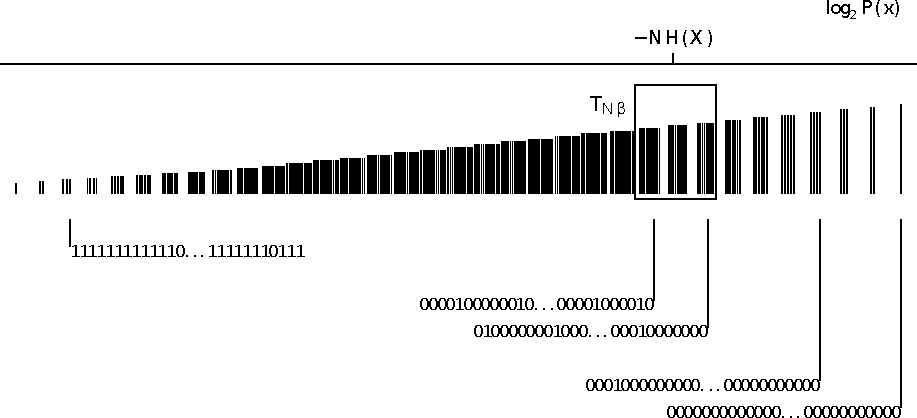
\includegraphics[width=0.5\textwidth]{images/seq100mackay3.pdf}
  \caption{Diagrama esquemático ilustrando todas as sequencias no conjunto $\mathcal{X}^n$ ordenadas pela probabilidade \cite{mackay2003}.}
  \label{fig:seq100mackay3}
  \end{figure}


  O termo \textbf{equipartição} é utilizado para descrever a ideia de que os membros do conjunto típico
  possuem aproximadamente a mesma probabilidade.

  
\end{frame}






\bibliographystyle{apalike}
\bibliography{bibliografia}
\label{bibliografia}

\end{document}

